\chapter{INSERT FINAL SNASE TITLE HERE}\label{snase}

\newcommand{\dpKa}{{\textDelta\pKa{}}}

%The changes in \pKa{} of titratable residues have long been used as reporters of local electrostatic environments in proteins. 
%Though \pKa{} shifts are difficult to interpret because of the perturbative nature of the probe and sensitivity to non-Coulombic effects such as hydrogen bonding, significant effort has been dedicated to developing computational electrostatic models based on experimentally measured shifts in \pKa{}. 
%Nitrile vibrational probes are potentially less disruptive and more direct reporters of local electrostatic environments, but quantitative interpretation is similarly convoluted by the ability of nitrile groups to accept a hydrogen bond. 
%We address these questions by comparing \pKa{} shifts and nitrile frequencies in the same positions in the same protein and elucidated the role of local interactions in determining nitrile mean vibrational frequency and line shape. 
%To this end, we incorporated nitrile probes into 10 locations of the staphylococcal nuclease (SNase) model protein where \pKa{} shifts had already been reported. 
%We report that nitrile frequencies and pKa shifts do not correlate in this system. 
%We characterized the local environment of each nitrile probe experimentally and with molecular dynamics simulations and show that hydrogen bonding interactions dominate the spectral line shapes. 
%We demonstrate that the information provided by the line shape of the nitrile spectra, compared to scalar values of pKa shift, describes local environments in proteins in a manner that will be useful for future computational efforts to predict electrostatics in complex biological systems.
%
%Significance Statement 
%The understanding and accurate prediction of electrostatic forces in proteins is a long-standing goal of the biophysics community, with implications for understanding protein function, improving drug discovery, and directing protein engineering. 
%Experimental methods for measuring electrostatic fields in proteins have relied on \pKa{} shifts in spite of the difficulty of their interpretation. 
%These measurements have been used to validate computational strategies for calculating electric field in proteins, with the assumption that \pKa{} shifts are predominantly due to electrostatics. 
%Here, we demonstrate that \pKa{} shifts do not agree with nitrile vibrational frequency shifts, a more direct probe of electrostatics, when measured in the same positions in staphylococcal nuclease, and we discuss the implications of using vibrational probes to benchmark computational efforts.

%%%%%%%%%%%%%%%%%%%%%%%%%%%%%%%%%%%%%%%%%%%%%%%%%%%%%%%%%%%%%%%%
%%%%%%%%%%%%%%%%%%%%%%%%%%%%%%%%%%%%%%%%%%%%%%%%%%%%%%%%%%%%%%%%
\section{Publication note} \label{snase-pub-note}
%%%%%%%%%%%%%%%%%%%%%%%%%%%%%%%%%%%%%%%%%%%%%%%%%%%%%%%%%%%%%%%%
%%%%%%%%%%%%%%%%%%%%%%%%%%%%%%%%%%%%%%%%%%%%%%%%%%%%%%%%%%%%%%%%

Portions of this chapter are adapted from the following publication:

\noindent Jeremy T. First, Elisa T. Novelli, Lauren J. Webb; Disagreement Between \pKa{} and Nitrile Vibrational Probes of Electrostatics: Experiments and Simulations in Staphylococcal Nuclease Demonstrate the Importance of Local interactions. emph{Proceedings of the National Academy of Sciences}. \textbf{2019}, \emph{Submitted}. 

JTF performed all calculations.
All code, force field parameters, structures, and other starting files used for the simulation, analysis, processing of data, and figure generation can be accessed at:
\url{https://github.com/jeremyfirst22/SNase_Nitriles}. 
Baseline correction and Gaussian fitting code can be accessed at: 
\url{https://github.com/jeremyfirst22/spectra_fitting}. 
ETN performed all experiments. The experimental methods are ommited from this Chapter, but they may be found in the publication.

%%%%%%%%%%%%%%%%%%%%%%%%%%%%%%%%%%%%%%%%%%%%%%%%%%%%%%%%%%%%%%%%
%%%%%%%%%%%%%%%%%%%%%%%%%%%%%%%%%%%%%%%%%%%%%%%%%%%%%%%%%%%%%%%%
\section{Introduction} \label{snase-intro}
%%%%%%%%%%%%%%%%%%%%%%%%%%%%%%%%%%%%%%%%%%%%%%%%%%%%%%%%%%%%%%%%
%%%%%%%%%%%%%%%%%%%%%%%%%%%%%%%%%%%%%%%%%%%%%%%%%%%%%%%%%%%%%%%%

Electrostatic forces play a critical role in biological phenomena and are of long-standing interest to the biophysical community. 
In proteins, for example, biochemical processes such as folding, catalysis, and intramolecular interactions are regulated by electric fields resulting from the arrangement of partial charges on each of the many thousands of atoms within the protein structure \cite{Honig1995}. 
Understanding the molecular detail of the structure, dynamics, and function of proteins therefore depends on accurate, quantitative experiments and calculations of highly heterogeneous electric fields inherent in protein structures \cite{Warshel1978}. 
However, because the Coulombic interactions between partially charged atoms decay over relatively long distances compared to other intermolecular forces, the sheer complexity of the system often makes electrostatic fields in proteins difficult to measure experimentally or predict computationally.

A common strategy for addressing this problem experimentally is to measure the change in \pKa{} (\dpKa{}) of ionizable amino acid side chains in a protein interior compared to the \pKa{} of the isolated amino acid in water \cite{Bradbury1966, Forsyth2002, Isom2010, Langsetmo1991, Markley1975}. 
The local distribution of partial charges in the protein in the immediate area around the ionizable residue can electrostatically stabilize or destabilize the charged state of the amino acid relative to the neutral state. 
This electrostatic effect changes the free energy of the proton transfer process and shifts the equilibrium according to Equation \ref{eq:snase-dpKa}:
\begin{equation}
    \Delta \pKa{} = \frac{\Delta \Delta G}{R T \ln(10)}
\label{eq:snase-dpKa}
\end{equation}
where $\Delta \Delta G$ is the change in the free energy of the proton transfer reaction, $R$ is the ideal gas constant, and $T$ is the temperature. 
Experimentally, \dpKa{} values can be measured in a variety of ways, such as with NMR chemical shifts and pH dependent thermodynamic stability experiments \cite{Bradbury1966, Markley1975, Isom2008}. 
A large number of \pKa{} shifts of ionizable residues in  many proteins have been collected and reported \cite{Grimsley2009}. 
In particular, Garcia-Moreno and coworkers systematically mutated several ionizable residues into 25 buried locations of a highly stable engineered variant of staphylococcal nuclease (SNase $\Delta+$PHS, hereafter referred to simply as ``SNase''). 
Using these \pKa{} probes, the authors measured shifts of up to $\sim$6 pH units towards the neutral state that reflected the solvent accessibility of the probe in the protein environment \cite{Isom2010, Isom2008, Harms2009, Isom2011}. 

This dataset has since been used as a common target to validate different computational electrostatic models \cite{Liu2018, Nielsen2011}. 
A notable coordinated effort towards this goal, known as the \pKa{} Cooperative, compared predicted \pKa{} shifts to the experimental \pKa{} shifts measured in SNase by the Garcia-Moreno group. 
Because of the complexity of the electrostatic environment in proteins, accurately modeling the effects of the electric fields require either a prohibitively expensive calculation or a significant oversimplification of the physical properties of the system. 
Consequently, the inability of many of these models to accurately reproduce the measured \pKa{} shifts demonstrated the challenge for current computational strategies to adequately model electrostatic interactions in proteins. 
The computational results produced by the \pKa{} Cooperative were typically able to predict the direction of the \pKa{} shift but not the magnitude, and in some cases were off by several pH units, indicating substantial uncertainty in the equilibrium protonation state of the titratable residue \cite{Alexov2011, Brooks2011}. 
While efforts to benchmark computational strategies against a common experimental database are promising, the measurement of a \pKa{} shift in itself is an oversimplification of the diverse interactions in a protein interior. 
One of the most significant issues is that shifts in \pKa{} are not direct measurements of electric field. 
Instead, they represent a change in stability that is dependent on a variety of factors other than electrostatic stabilization, such as hydrogen bonding or salt-bridge stabilization of a charged state. 
Further, a measured \pKa{} value is a single scalar quantity that represents an ensemble average of a highly dynamic and heterogeneous electrostatic environment. 

Our laboratory has been interested in building a dataset with spectroscopic measurements that are directly correlated to electric field and could serve as an alternative benchmark for efforts to design, test, and validate computational models and strategies. 
Along with other laboratories, we have been pursuing vibrational Stark effect (VSE) spectroscopy of protein-bound nitrile probes to measure electric fields in biological systems \cite{Choi2008, Fried2015, Getahun2003, Johnson2014, McMahon2010, Oh2008, Park2000, Slocum2018, Stafford2010, Suydam2003, Waegele2009, Walker2013}. 
Nitriles are convenient biomolecular probes because they are small, absorb in an uncluttered region of the protein vibrational spectrum, have reasonable oscillator strength, and can be incorporated virtually anywhere within a biomolecular structure \cite{Getahun2003, Fafarman2006, Kirshenbaum2002, Webb2008}. 
Vibrational spectra of nitriles have been collected in a variety of biologically relevant environments such as lipid membranes, protein interiors, protein-protein interfaces, and protein active sites \cite{Shrestha2017, Slocum2016, Stafford2012, Walker2014}. 
Shifts in the vibrational energy of nitrile groups can be directly related to local electric field through the linear Stark equation \cite{Fafarman2010, Shields2000}:
\begin{equation}
\Delta E = hc \Delta \nu = - \Delta \vec{\mu} \cdot \Delta \vec{F}
\label{eq:snase-stark}
\end{equation}
where $\Delta E$ is the change in absorption energy of the chromophore in response to a change in local electric field, $\Delta \vec{F}$. 
$\Delta \vec{\mu}$ is the difference dipole moment of the vibrational transition. 
For nitriles in particular, $\Delta \vec{\mu}$ has been well-characterized \cite{Suydam2003, Andrews2000, Andrews2002}. 
Through this equation we can directly interpret differences in vibrational energy as differences in the magnitude and direction of the local electric field in the immediate vicinity of the nitrile. 
Previously, in superfolder green fluorescent protein (GFP), we have shown that three separate measurements of electrostatic environment (\pKa{} shifts of the titratable fluorophore, linear electronic Stark shifts of the fluorophore, and VSE shifts of a nearby nitrile probe) all responded similarly to changes in electric field made by amino acid mutations near the fluorophore \cite{Slocum2017}. 
This led us to the conclusion that the vibrational spectra of nitrile probes could be used as an orthogonal measurement of electric field to \pKa{} shifts, augmenting the datasets used for benchmarking electrostatic models in future computational studies.

One major caveat to the above interpretation of nitrile spectra is that nitriles can accept hydrogen bonds, which causes frequency shifts that are inherently quantum mechanical and thus not described by Equation \ref{eq:snase-stark} \cite{Slocum2018}. 
Moreover, the specific geometry of the hydrogen bonding interaction changes the magnitude and direction of the frequency shift. 
\emph{Ab initio} calculations by Choi et al. showed that linear, \textsigma-hydrogen bonds blue shift the nitrile frequency by withdrawing electron density from an antibonding orbital of the C$\equiv$N bond, and perpendicular, \textpi-hydrogen bonds red shift the nitrile frequency by withdrawing electron density from a bonding orbital \cite{Choi2008}. 
Recently, we demonstrated that these contributions from hydrogen bonding can dominate the observed frequency of nitrile probes in GFP, and therefore interpretations of nitrile frequency according to Equation \ref{eq:snase-stark} require careful control experiments, often coupled with molecular dynamics (MD) simulations, to reveal the extent of potential hydrogen bonding interactions \cite{First2018}. 

This complication is not unique to nitrile vibrational probes, however, because \pKa{} probes are similarly affected by local interactions. 
The proton transfer process of a \pKa{} probe adds or removes a hydrogen that may be involved in hydrogen bonding. 
Nearby hydrogen bond interactions may preferentially stabilize either the charged or neutral state of the probe, affecting the observed \dpKa{}. 
Further, since all titratable amino acids have multiple potential hydrogen bond donors or acceptors, the stabilization effect of hydrogen bonding on either the charged or neutral state of a \pKa{} probe is likely more difficult to predict than for nitriles, which only have one lone pair of electrons that may participate in hydrogen bonding. 

Because both \pKa{} and nitrile probes are affected by hydrogen bonding interactions, it has been suggested that they are mostly measuring changes in the level of solvation \cite{Adhikary2014, Adhikary2015, Simonson2004}. 
While the level of solvation certainly plays a role in both \dpKa{} measurements and nitrile vibrational frequencies, the difference in solvation energy between the charged and the neutral state of an amino acid is significantly more substantial than the difference between solvation energy of the ground and vibrationally excited state of the same molecule. 
In our recent study of hydrogen bonding to nitriles in GFP, we attempted to resolve some of the challenges of the local effects on nitrile oscillators by demonstrating that the frequency temperature line slope (FTLS) of the nitrile absorption energy was a quantitative tool for measuring hydrogen bonding, as had been postulated by Adhikary et al. \cite{First2018, Adhikary2015}. 
We further demonstrated the necessity of such a tool; 
in that system, the hydrogen bonding contribution to the nitrile frequency dominated the absorption frequency, and every single probe location experienced hydrogen bonding. 
Nevertheless, this work demonstrated that, by accounting for the hydrogen bonding contribution to the nitrile absorption spectra, the absorption energy can be interpreted as a VSE shift according to Eq \ref{eq:snase-stark}.

Both \dpKa{} and VSE measurements of electric field require a site-specific molecular probe. 
\pKa{} probes are limited in that they must be titratable and the probe must change its charge state during the measurements. 
Large scale conformational changes of the protein around the charged state can convolute the interpretation of the \pKa{} measurement \cite{Isom2010, Isom2011, Harms2011}. 
In contrast, VSE probes are sensitive to more subtle electrostatic perturbations and only rely on a vibrational transition. 
While the dipole moment changes between the ground and excited vibrational states, this difference perturbs the protein structure significantly less, and because nitrile groups are small, the insertion of a nitrile is minimally disruptive to the protein structure \cite{Dippel2016}.

Additional work in our laboratory has focused on the calculation of electric fields from MD simulations in order to reproduce the nitrile frequencies. 
Our efforts have primarily followed two strategies: 
1) direct computation of the field at the midpoint of the nitrile using the MD force field; and 
2) continuum electrostatics calculations of the potential using the Poisson-Boltzmann (PB) equation. 
For the most part, the results of these calculations have not been able to capture the measured nitrile absorption energies \cite{Ritchie2013, Ritchie2014, Ritchie2015}. 
We hypothesize that this is due to two factors: 
1) the convolution of hydrogen-bonding effects and VSE shifts; and 
2) the fact that MD force fields are parameterized to accurately sample structural ensembles at room temperature but are not intended to quantitatively reproduce forces. 
More sophisticated models, such as the SolEFP model, have had more success in quantitatively capturing the vibrational shifts of nitriles and reproducing the line shapes of the vibrational spectra \cite{Blasiak2013, Blasiak2016}. 
However, such models are often computationally intensive and require specialized software and expertise to implement. 
It is therefore still desirable to develop a simpler model using widely available tools to interpret vibrational spectra. 

Here, we report nitrile absorption measurements of cyanocysteine (CNC) nitrile probes in 10 locations in SNase (illustrated in Figure \ref{fig:snase-system}) at sites where previous \dpKa{} measurements have been reported. 
We show that there is poor correlation between the nitrile absorption frequencies and the previously published \dpKa{} values at the same locations within the protein, indicating the inequality of these two data sets. 
We hypothesize that the differences between the two measurements are due to differences in the response of each molecular probe to local interactions. 
Using temperature-dependent Fourier transform infrared spectroscopy (FTIR) experiments and MD simulations, we provide evidence that the FTLS is a quantitative measurement of the hydrogen bonding status of nitrile probes \cite{First2018}. 
Further, we used MD simulations to interpret the line shapes of the nitrile spectra by comparing them to calculated electric fields. 
While the average calculated fields were not correlated to the vibrational frequencies, the distribution of the fields qualitatively described the line shape of the experimental spectra. 
Overall, though we show that \dpKa{} and nitrile vibrational frequencies are not equivalent and both measurements are convoluted by local effects such as hydrogen bonding, the information contained in the line shapes of the nitrile spectra are valuable for understanding the electrostatic environment around the probe. 
Further, in the case of nitrile probes, additional experiments such as FTLS provide a diagnostic tool for quantifying the extent of hydrogen bonding to the nitrile. 
The additional information contained in the line width and specific line shape of nitrile vibrational spectra provide a more robust, self-consistent experimental dataset that enables the quantitative interpretation of electrostatics. 
These data can be used to benchmark electrostatic models and improve the prediction and understanding of complex electric fields in biological systems.  

\begin{figure}
    \center
    \includegraphics[width=\single]{figures-snase/nitrile_locations.png}
    \caption[Locations of the nitrile probes in staphylococcal nuclease]{
        Locations of the nitrile probes in staphylococcal nuclease (SNase). 
        Each location represented by the colored spheres was independently mutated to a cysteine, which was cyanylated through post-translational modification to cyanocysteine (CNC). 
        The first letter indicates the one letter code of the WT residue that was replaced by CNC, denoted by ``X''. 
        The dark gray ribbon shows the backbone of SNase, and the white sphere shows the location of the native \ce{Ca^2+} ion. 
    }
    \label{fig:snase-system}
\end{figure}

%%%%%%%%%%%%%%%%%%%%%%%%%%%%%%%%%%%%%%%%%%%%%%%%%%%%%%%%%%%%%%%%
%%%%%%%%%%%%%%%%%%%%%%%%%%%%%%%%%%%%%%%%%%%%%%%%%%%%%%%%%%%%%%%%
\section{Methods} \label{snase-methods}
%%%%%%%%%%%%%%%%%%%%%%%%%%%%%%%%%%%%%%%%%%%%%%%%%%%%%%%%%%%%%%%%
%%%%%%%%%%%%%%%%%%%%%%%%%%%%%%%%%%%%%%%%%%%%%%%%%%%%%%%%%%%%%%%%

%\subsection{Mutagenesis, Expression, and Purification}
%
%Five pET42a plasmids containing the $\Delta+$PHS variant of SNase and a mutation, either V23C, L38C, T62C, V66C, or I92C, were generous gifts of Bertrand Garcia-Moreno. 
%The $\Delta+$PHS variant denotes a deletion of residues 44-49, and the mutations P117G, H124L, S128A, G50F, and V51N, as previously described \cite{Garcia-Moreno1997}. 
%Additional mutations were made by reverting the I92C mutant-containing plasmid to the wild type Ile, and then making five additional mutated constructs: L25C, A58C, A90C, A109C, and N118C. 
%All site-directed mutagenesis was carried out via the QuikChange Lightning kit (Agilent).
%
%The mutated plasmids were transformed into BL21-DE3 cells (New England BioLabs) and grown in LB-Broth containing kanamycin at 37 \si{\celsius} until the OD$_{600}$ reached 0.4-0.6. 
%Cells were induced with 1 mM isopropyl \textbeta-D-1-thiogalactopyranoside (IPTG) for 4-6 hours, collected by centrifugation, flash frozen in liquid nitrogen, and stored at -80\si{\celsius} for further use. 
%Protein was purified from inclusion bodies based on a strategy described previously \cite{Shortle1989}. 
%Briefly, cells were lysed by re-suspending in Buffer A containing 6 M urea, 25 mM Tris, and 2.5 mM EDTA, pH 8. 
%Cell debris and inclusion bodies were collected by centrifugation, and protein was freed from inclusion bodies by resuspending the pellet in Buffer B (same as buffer A with the addition of 400 mM NaCl) for 30 minutes and then centrifuging again. 
%Unfolded protein in the supernatant was collected and purified by two successive ethanol precipitation steps followed by further purification with cation exchange chromatography (SP sepharose, GE Healthcare) using Buffer A as the loading buffer and Buffer B as the elution buffer. 
%The eluent containing SNase was precipitated a final time with ethanol, then resuspended in fresh Buffer B, and the CNC probe was incorporated into the unfolded protein as previously described \cite{Fafarman2006}.
%The protein was then refolded by dialyzing overnight against 1 M KCl, followed by dialyzing twice for 2 hours each against deionized \ce{H2O}, and overnight again with deionized \ce{H2O}. 
%Purified and refolded protein was diluted to 300 $\mu${}M with deionized \ce{H2O}, separated into 1 mL aliquots, and flash frozen and stored at -80 \si{\celsius} for further use. 
%Prior to use, the protein samples were exchanged into 10 mM \ce{CaCl2}. 
%Protein refolding was confirmed by circular dichroism (CD) spectroscopy, and the incorporation of the nitrile label, which results in a 26 Da increase in protein mass, was confirmed with mass spectrometry.
%
%\subsection{Fourier Transform Infrared Spectroscopy}
%
%All FTIR spectra were collected on a Bruker Vertex 70 instrument with an InSb detector at a resolution of 0.5 \si{\wn}. 
%Room temperature experiments were measured in a liquid cell with sapphire windows (Meller Optics) separated by 125 $\mu$M teflon spacers. 
%Each run consisted of 250 scans. 
%Temperature dependent IR was collected in a temperature controlled liquid cell with sapphire windows separated by 100 $\mu$M teflon spacers. 
%To generate equivalent signal-to-noise ratios as the room temperature experiments, these runs consisted of 600 scans. 

\subsection{Baseline correction and spectra fitting}

All spectra were baseline corrected by fitting a 5th order spline function to the baseline. 
The maxima of the baseline corrected spectra were normalized to 1 and fit to a single or double Gaussian function. 
The average maximum of these fits are the reported vibrational frequencies in Table \ref{tbl:snase-ftir} and Table \ref{tbl:snase-ftls}. 
In all cases, reported values are the average of at least three measurements.

\subsection{Molecular dynamics simulations}

A template SNase protein structure bound to \ce{Ca^2+} was modeled by homology from the pdb:3bdc crystal structure using the MODELLER software package \cite{Castaneda2009, Mari-Renom2000}. 
From this structure, 10 separate mutations from the WT residue to cysteine were made using the mutagenesis tool in PyMol at each of the selected probe locations \cite{DeLano2002}. 
Using the Avogadro molecular editing package, the mutated cysteine was further modified to cyanocysteine (CNC) and independently minimized \cite{Hanwell2012}. 
Parameters for the CNC residue have been described previously \cite{Stafford2010, Ensign2011}. 
All further minimizations and MD simulations were performed using the Gromacs 2016.3 molecular dynamics simulation package\cite{Abraham2015, Berendsen1995, Hess2008, Lindahl2001, Pall2015, Pronk2013, VanDerSpoel20015} and the Amber03 force field \cite{Duan2003, Sorin2005}.

Each of the 10 protein systems was energy minimized in a vacuum using the steepest descent algorithm and then solvated in a dodecahedron box of TIP3P water, with a minimum distance of protein to the edge of the box of 1.5 nm \cite{Jorgenson1983}. 
The solvated systems were then energy minimized using a steepest descent approach, heated under the NVT ensemble at 300 K, and then equilibrated under the NPT ensemble at 1 atm. 
Production MD was run on each equilibrated system for 100 ns, using the same simulation parameters as described previously \cite{First2018}, and a snapshot was saved every 4 ps.

%%%%%%%%%%%%%%%%%%%%%%%%%%%%%%%%%%%%%%%%%%%%%%%%%%%%%%%%%%%%%%%%
%%%%%%%%%%%%%%%%%%%%%%%%%%%%%%%%%%%%%%%%%%%%%%%%%%%%%%%%%%%%%%%%
\section{Results and Discussion} \label{snase-results}
%%%%%%%%%%%%%%%%%%%%%%%%%%%%%%%%%%%%%%%%%%%%%%%%%%%%%%%%%%%%%%%%
%%%%%%%%%%%%%%%%%%%%%%%%%%%%%%%%%%%%%%%%%%%%%%%%%%%%%%%%%%%%%%%%

\subsection{Nitrile and \pKa{} probes respond differently to local interactions}

Measuring the \pKa{} shifts of either WT or mutated ionizable residues has long been a strategy for estimating the effect of electrostatic forces, such as charge separation and apparent dielectric, in proteins. 
More recently, vibrational spectroscopy of nitriles placed site-specifically in proteins has been an alternative method for quantifying electrostatic effects in protein systems. 
In order to compare the merits of the two strategies, we incorporated CNC nitrile probes into 10 separate locations in SNase (illustrated in Figure \ref{fig:snase-system}) for which there are already reported values of \dpKa{} \cite{Isom2010, Isom2011}. 
These 10 positions were chosen to represent the full range of \pKa{} shifts measured by Garcia-Moreno and coworkers, as well as to sample the spatial diversity in the interior of SNase.

For each of the ten nitrile-containing protein systems, FTIR spectra were collected; 
average spectra are shown in Figure \ref{fig:snase-ftir}. 
The average and standard deviation of the peak frequencies for each nitrile location are given in Table \ref{tbl:snase-ftir}. 
Additionally, we collected the FTIR spectra of methylthiocyanate (MeSCN) dissolved in \ce{H2O} and in DMSO, which served as standards for representing a nitrile probe in protic and aprotic environments, respectively. 
Standard deviations of the nitrile frequency measurements were all generally within 0.1 \si{\wn}. 
For MeSCN in \ce{H2O} and DMSO, we measured nitrile frequencies of 2162.60 and 2153.44 \si{\wn}, respectively. 
The most red-shifted peak, A90X, had a mean frequency of 2156.58 \si{\wn}. 
V66X was nearly as red-shifted with a mean frequency of 2157.16 \si{\wn}. 
The full width at half maxima (FWHM) of the spectra, which qualitatively describe the environmental heterogeneity experienced by a probe, were small: 4.18 \si{\wn} and 3.38 \si{\wn}, respectively. 
This suggests that these two probes were in a homogeneous environment at those positions. 
A109X and T62X were relatively red-shifted compared to MeSCN in \ce{H2O}, with mean frequencies of 2159.46 \si{\wn} and 2159.96 \si{\wn}, respectively. 
The FWHMs of these two probe locations were larger than both A90X and V66X. 
A109X showed a broad absorption peak (10.05 \si{\wn}), while T62X was not as broad (5.63 \si{\wn}) but had a significant shoulder red-shifted from the absorption maximum, suggesting that this probe experienced at least two different chemical environments. 
V23X and L25X had mean frequencies in the middle of our data set (2160.18 \si{\wn} and 2161.38 \si{\wn}, respectively) and were both fairly narrow (FWHMs of 3.86 \si{\wn} and 4.98 \si{\wn}, respectively). 
Interestingly, the L25X peak appeared slightly wider than a single Gaussian, suggesting the possibility of two close and equally represented populations contributing to the overall line shape. 
L38X and I92X had similar mean frequencies (2161.89 \si{\wn} and 2162.06 \si{\wn}, respectively) but different line shapes. 
L38X had a broad peak, with FWHM of 8.36 \si{\wn}, indicating heterogeneity in the environment sampled by the probe. 
By contrast, I92X had a narrow peak (4.34 \si{\wn}) suggesting that the probe experienced a homogeneous environment. 
The most blue-shifted peaks, N118X and A58X (2162.27 \si{\wn} and 2163.20 \si{\wn}, respectively) were both very broad (FWHMs of 15.27 \si{\wn} and 14.71 \si{\wn}, respectively), indicating the probe sampled a heterogeneous environment. 
Collectively, nitrile spectra from these 10 locations within the same protein displayed the diverse range of spectroscopic results possible from measuring electric fields in a biological sample. 

\begin{figure}
    \center
    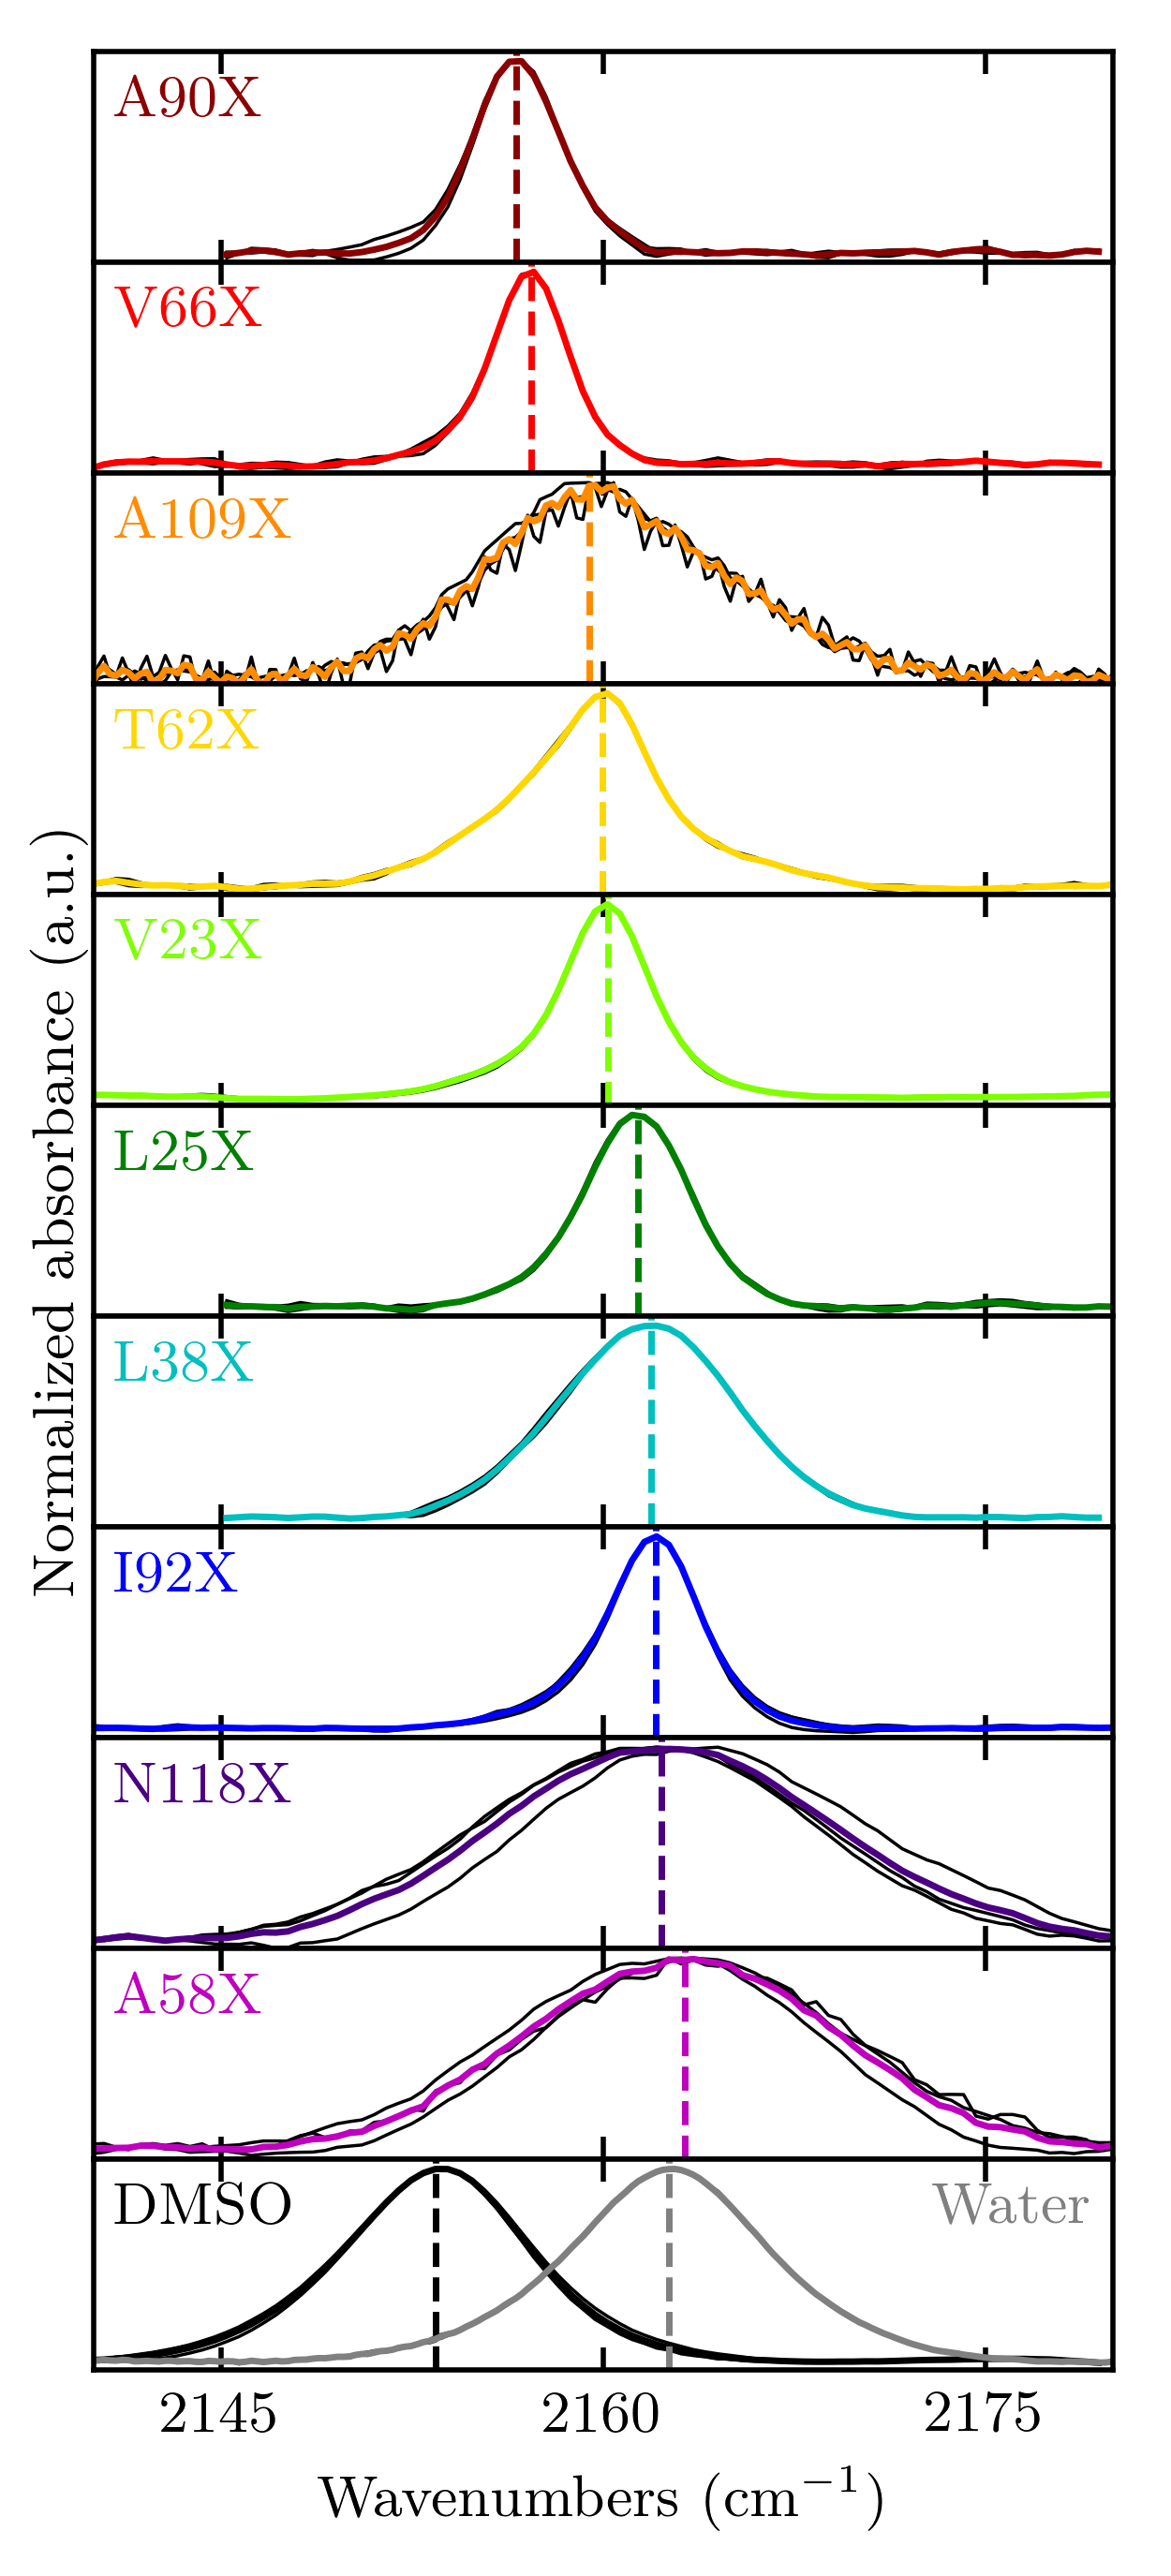
\includegraphics[width=2.75in]{figures-snase/spectra.png}
    \caption[FTIR absorption spectra of each CNC incorporated in SNase]{
        FTIR absorption spectra of CNC incorporated at each of the ten locations shown in Figure \ref{fig:snase-system} at room temperature, arranged from lowest mean frequency to highest mean frequency. 
        The spectra of MeSCN in both DMSO and water are included for comparison. 
        The maximum absorbance of each spectrum was normalized to 1. 
        Colored lines: averaged absorption spectra; 
        black traces: individual FTIR spectra (some traces lie directly underneath the colored lines); 
        vertical dashed lines: peak frequency of the averaged spectra reported in Table \ref{tbl:snase-ftir}.
    }
    \label{fig:snase-ftir}
\end{figure}

\begin{table}
    \caption[Summary of FTIR and \pKa{} measurements at ten locations in SNase]{
        Nitrile mean vibrational frequency, FWHM, and FTLS of nitrile probes, and corresponding \pKa{}s of lysine and glutamate probes at ten locations in the interior of SNase.
    }
    \begin{center}
        \resizebox{\double}{!}{
    \begin{tabular}{cccccc} 
    \toprule
    \rowcolor{lgray}
    Amino acid & \multicolumn{3}{c}{ Nitrile location} & \multicolumn{2}{c}{p$K_a$ probe location} \\
    \rowcolor{lgray}
        position & $\tilde{\nu}$ (\si{\wn})  & FWHM (\si{\wn}) &  FTLS (\si{\wn} \si{\celsius}$^{-1}$) & $^{a}$Lysine \pKa{} & $^{b}$Glutamate \pKa{} \\
    \cmidrule(r){1-1}\cmidrule(lr){2-4}\cmidrule(l){5-6}

A90X  &         $2156.58  \pm   0.05  $&$  4.18  \pm   0.23  $&$ -0.011    \pm  0.000  $&$ 8.6   $&$    6.4 $ \\
V66X  &         $2157.16  \pm   0.01  $&$  3.38  \pm   0.00  $&$ -0.006    \pm  0.000  $&$ 5.6   $&$    8.5 $ \\
A109X &         $2159.46  \pm   0.10  $&$ 10.05  \pm   0.60  $&$ -0.018    \pm  0.002  $&$ 9.2   $&$    7.9 $ \\
T62X  &         $2159.96  \pm   0.03  $&$  5.63  \pm   0.23  $&$ -0.014    \pm  0.001  $&$ 8.1   $&$    7.7 $ \\
V23X  &         $2160.18  \pm   0.00  $&$  3.86  \pm   0.00  $&$ -0.008    \pm  0.001  $&$ 7.3   $&$    7.1 $ \\
L25X  &         $2161.38  \pm   0.04  $&$  4.98  \pm   0.23  $&$ -0.008    \pm  0.001  $&$ 6.3   $&$    7.5 $ \\
L38X  &         $2161.89  \pm   0.03  $&$  8.36  \pm   0.23  $&$ -0.027    \pm  0.002  $&$ 10.4  $&$    6.8 $ \\
I92X  &         $2162.06  \pm   0.03  $&$  4.34  \pm   0.00  $&$ -0.016    \pm  0.000  $&$ 5.3   $&$    9.0 $ \\
N118X &         $2162.27  \pm   0.55  $&$ 15.27  \pm   0.23  $&$ -0.053    \pm  0.006  $&$ 10.4  $&$    4.5 $ \\
A58X  &         $2163.20  \pm   0.40  $&$ 14.71  \pm   0.34  $&$ -0.027    \pm  0.001  $&$ 10.4  $&$    7.7 $ \\
MeSCN in DMSO  &$2153.44  \pm   0.15  $&$  8.36  \pm   0.11  $&$ -0.008    \pm  0.004  $&$ --    $&$    --  $ \\
MeSCN in Water &$2162.60  \pm   0.03  $&$  9.00  \pm   0.11  $&$ -0.043    \pm  0.002  $&$ --    $&$    --  $ \\
    \bottomrule
    \end{tabular}
}
    \end{center}
    $^a$Lysine \pKa{} values adapted from ref \citenum{Isom2011} \\
    $^b$Glutamate \pKa{} values adapted from ref \citenum{Isom2010} \\
    All error values are reported as the standard deviation of at least 3 measurements
    \label{tbl:snase-ftir}
\end{table}

Because \pKa{} shifts are often used as a proxy for electrostatics to benchmark computational methods, we compared the \dpKa{} of buried lysine and glutamate residues published by Garcia-Moreno and coworkers against the measured nitrile frequencies at those same locations shown in Figure \ref{fig:snase-ftir} \cite{Isom2010, Isom2011}. 
Figure \ref{fig:snase-pKas_vs_peak} shows the comparison of our measured nitrile frequencies to the reported \pKa{} of lysine (Figure \ref{fig:snase-pKas_vs_peak}A) and glutamate (Figure \ref{fig:snase-pKas_vs_peak}B) incorporated at the same locations. 
In both plots, the horizontal dashed line represents the \pKa{} of the isolated amino acid in water, and the vertical dashed line represents the nitrile frequency of MeSCN in water. 
Therefore, the distance from the dashed line on both axes represents the deviation of the two different types of probes from their values in water. 
If the nitrile probes and the \pKa{} probes measured the same interactions, we would expect a correlation from least perturbed (where the two dashed lines intersect) to most perturbed. 
In the case of the lysine probe in Figure \ref{fig:snase-pKas_vs_peak}A, there was no such correlation ($r = 0.33$). 
In the case of the glutamate probe in Figure \ref{fig:snase-pKas_vs_peak}B, there was an even poorer correlation ($r = -0.12$). 
Together, these trends suggest that the \pKa{} probes and the nitrile probe responded to the same environment but with different contributions from local interactions. 
This is further supported by the fact that lysine and glutamate, though both \pKa{} probes, experienced different \dpKa{}s in the same locations, as shown in Figure \ref{fig:snase-pKas_vs_peak}C. 
For four of the probe locations, the measured \pKa{} shift of lysine did not agree with the measured \pKa{} shift of glutamate in the same position. 
This is not unique to the 10 nitrile locations investigated here; 
the remainder of the 25 locations measured by Garcia-Moreno and coworkers also do not correlate well (black diamonds in Figure \ref{fig:snase-pKas_vs_peak}C, $r = -0.69$). 
Because lysine and glutamate differ in charge, size, flexibility, polarity, and hydration, it is likely that while in the same protein location, the two different \pKa{} probes interacted differently with the surrounding protein structure \cite{Harms2009, Isom2011}, and thus knowing a \dpKa{} value for a particular location in a protein is not useful for determining the electrostatic environment. 
Furthermore, lysine and glutamate can participate in different hydrogen bonding interactions. 
The amine group on the side chain of lysine can donate up to three hydrogen bonds, while the carboxylate group of the glutamate side chain can accept multiple hydrogen bonds. 
These differences in possible local interactions likely lead to differences in the stability of the charged and neutral states between the two different \pKa{} probes, resulting in discrepancies in \dpKa{} that are not directly related to electric field. 
We will return to this observation later in the text.

\begin{figure}
    \center
    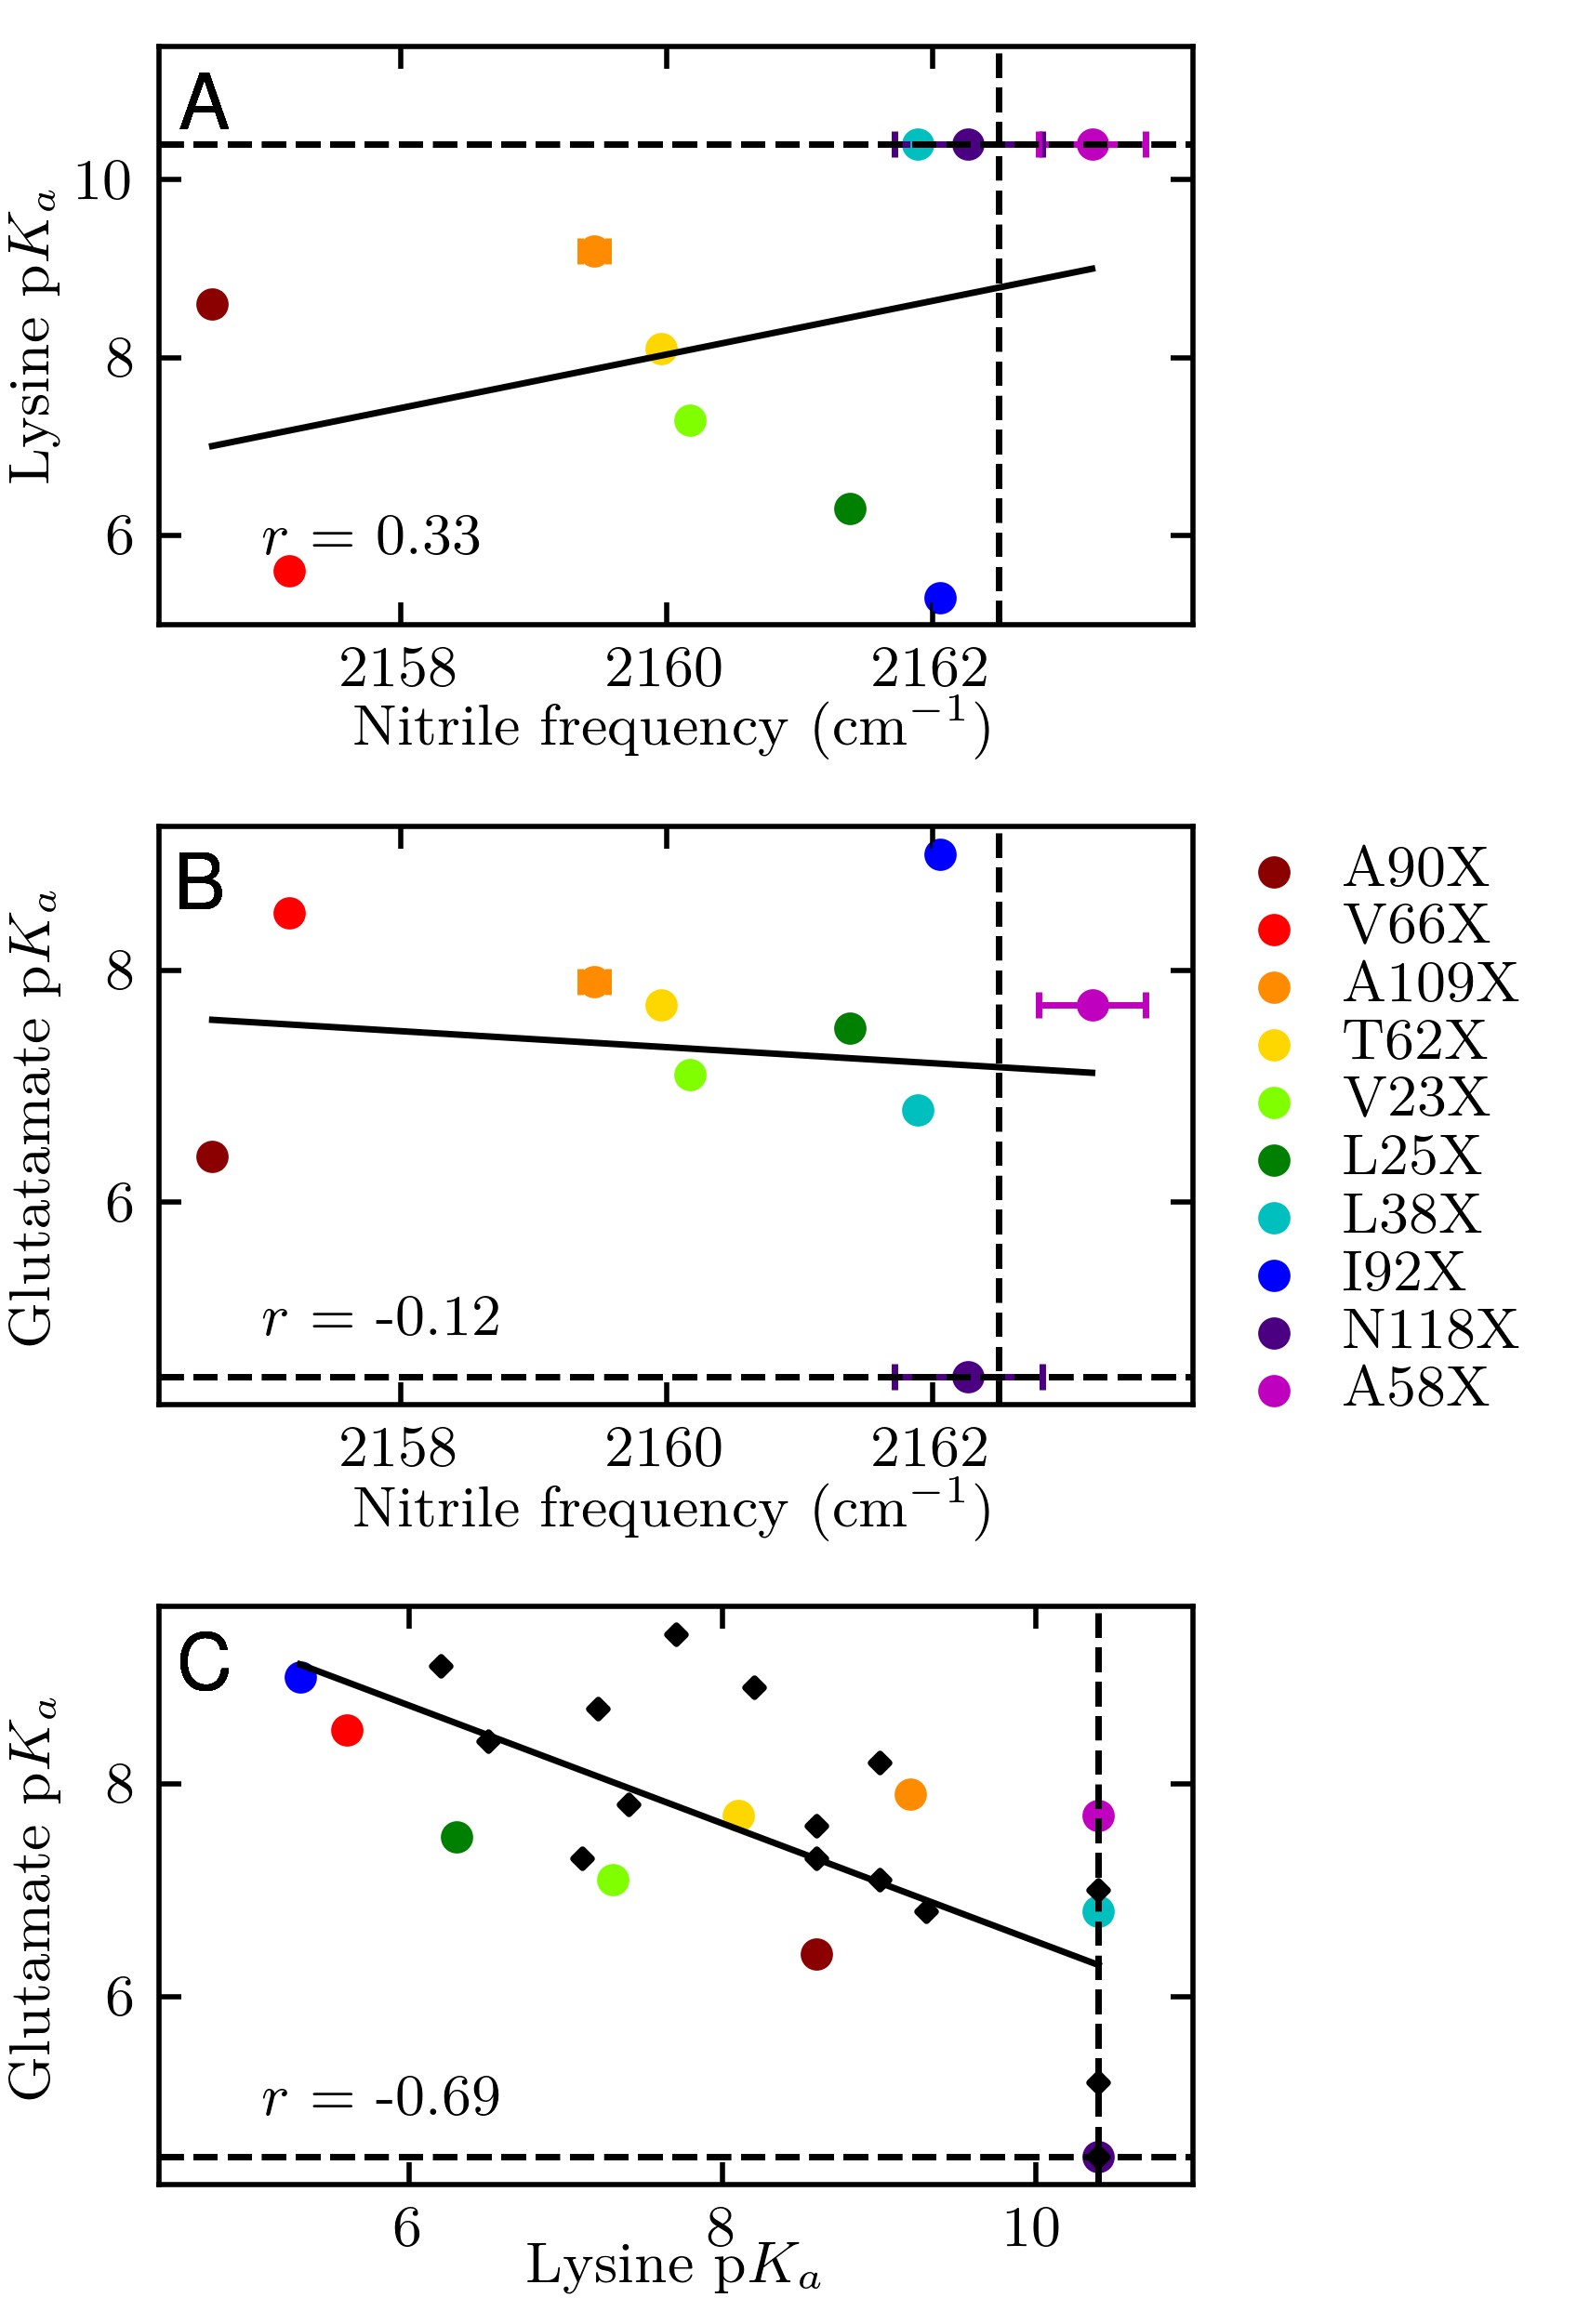
\includegraphics[width=\single]{figures-snase/pKa_vs_peak.png}
    \caption[Comparison of three molecular probes of electrostatics at 10 locations in SNase]{
        Comparison of three molecular probes of electrostatics at 10 locations in SNase. 
        (A) Reported values of \pKa{} of a lysine residue compared to the measured vibrational frequency of a CNC probe at the same position. 
        (B) Reported values of \pKa{} of a glutamate residue compared to the measured vibrational frequency of a CNC probe at the same position. 
        (C) Comparison of the reported values of \pKa{} as measured by lysine and glutamate \pKa{} probes. 
        Colored circles: the 10 constructs investigated in this work; 
        black diamonds: the remainder of positions reported by Garcia-Moreno and coworkers. 
        \pKa{} data reproduced from ref \citenum{Isom2010} and ref \citenum{Isom2011}. 
        Dashed lines: the vibrational frequency of MeSCN in water or the \pKa{} of either lysine or glutamate isolated in water. 
        Solid lines: Linear regression fits of the data.
    }
    \label{fig:snase-pKas_vs_peak}
\end{figure}

\subsection{Molecular dynamics simulations}

In order to investigate the presence of hydrogen bonds to the nitriles in our systems, we performed 100 ns MD simulations on each of the ten nitrile-containing proteins systems and on the WT SNase. 
First, we monitored the backbone RMSD of the crystalized residues (residues 7-141) for each nitrile-containing mutant construct and compared them to the WT protein. 
These data for each trajectory are shown in in Figure \ref{fig:snase-rmsd}. 
The backbone RMSD of the nitrile containing systems were all similar to that of the WT simulation, demonstrating that the nitrile perturbation to the local protein environment was small, at least on the time scale of the simulations, and that the simulations sufficiently sampled physically reasonable structures.

\begin{figure}
    \center
    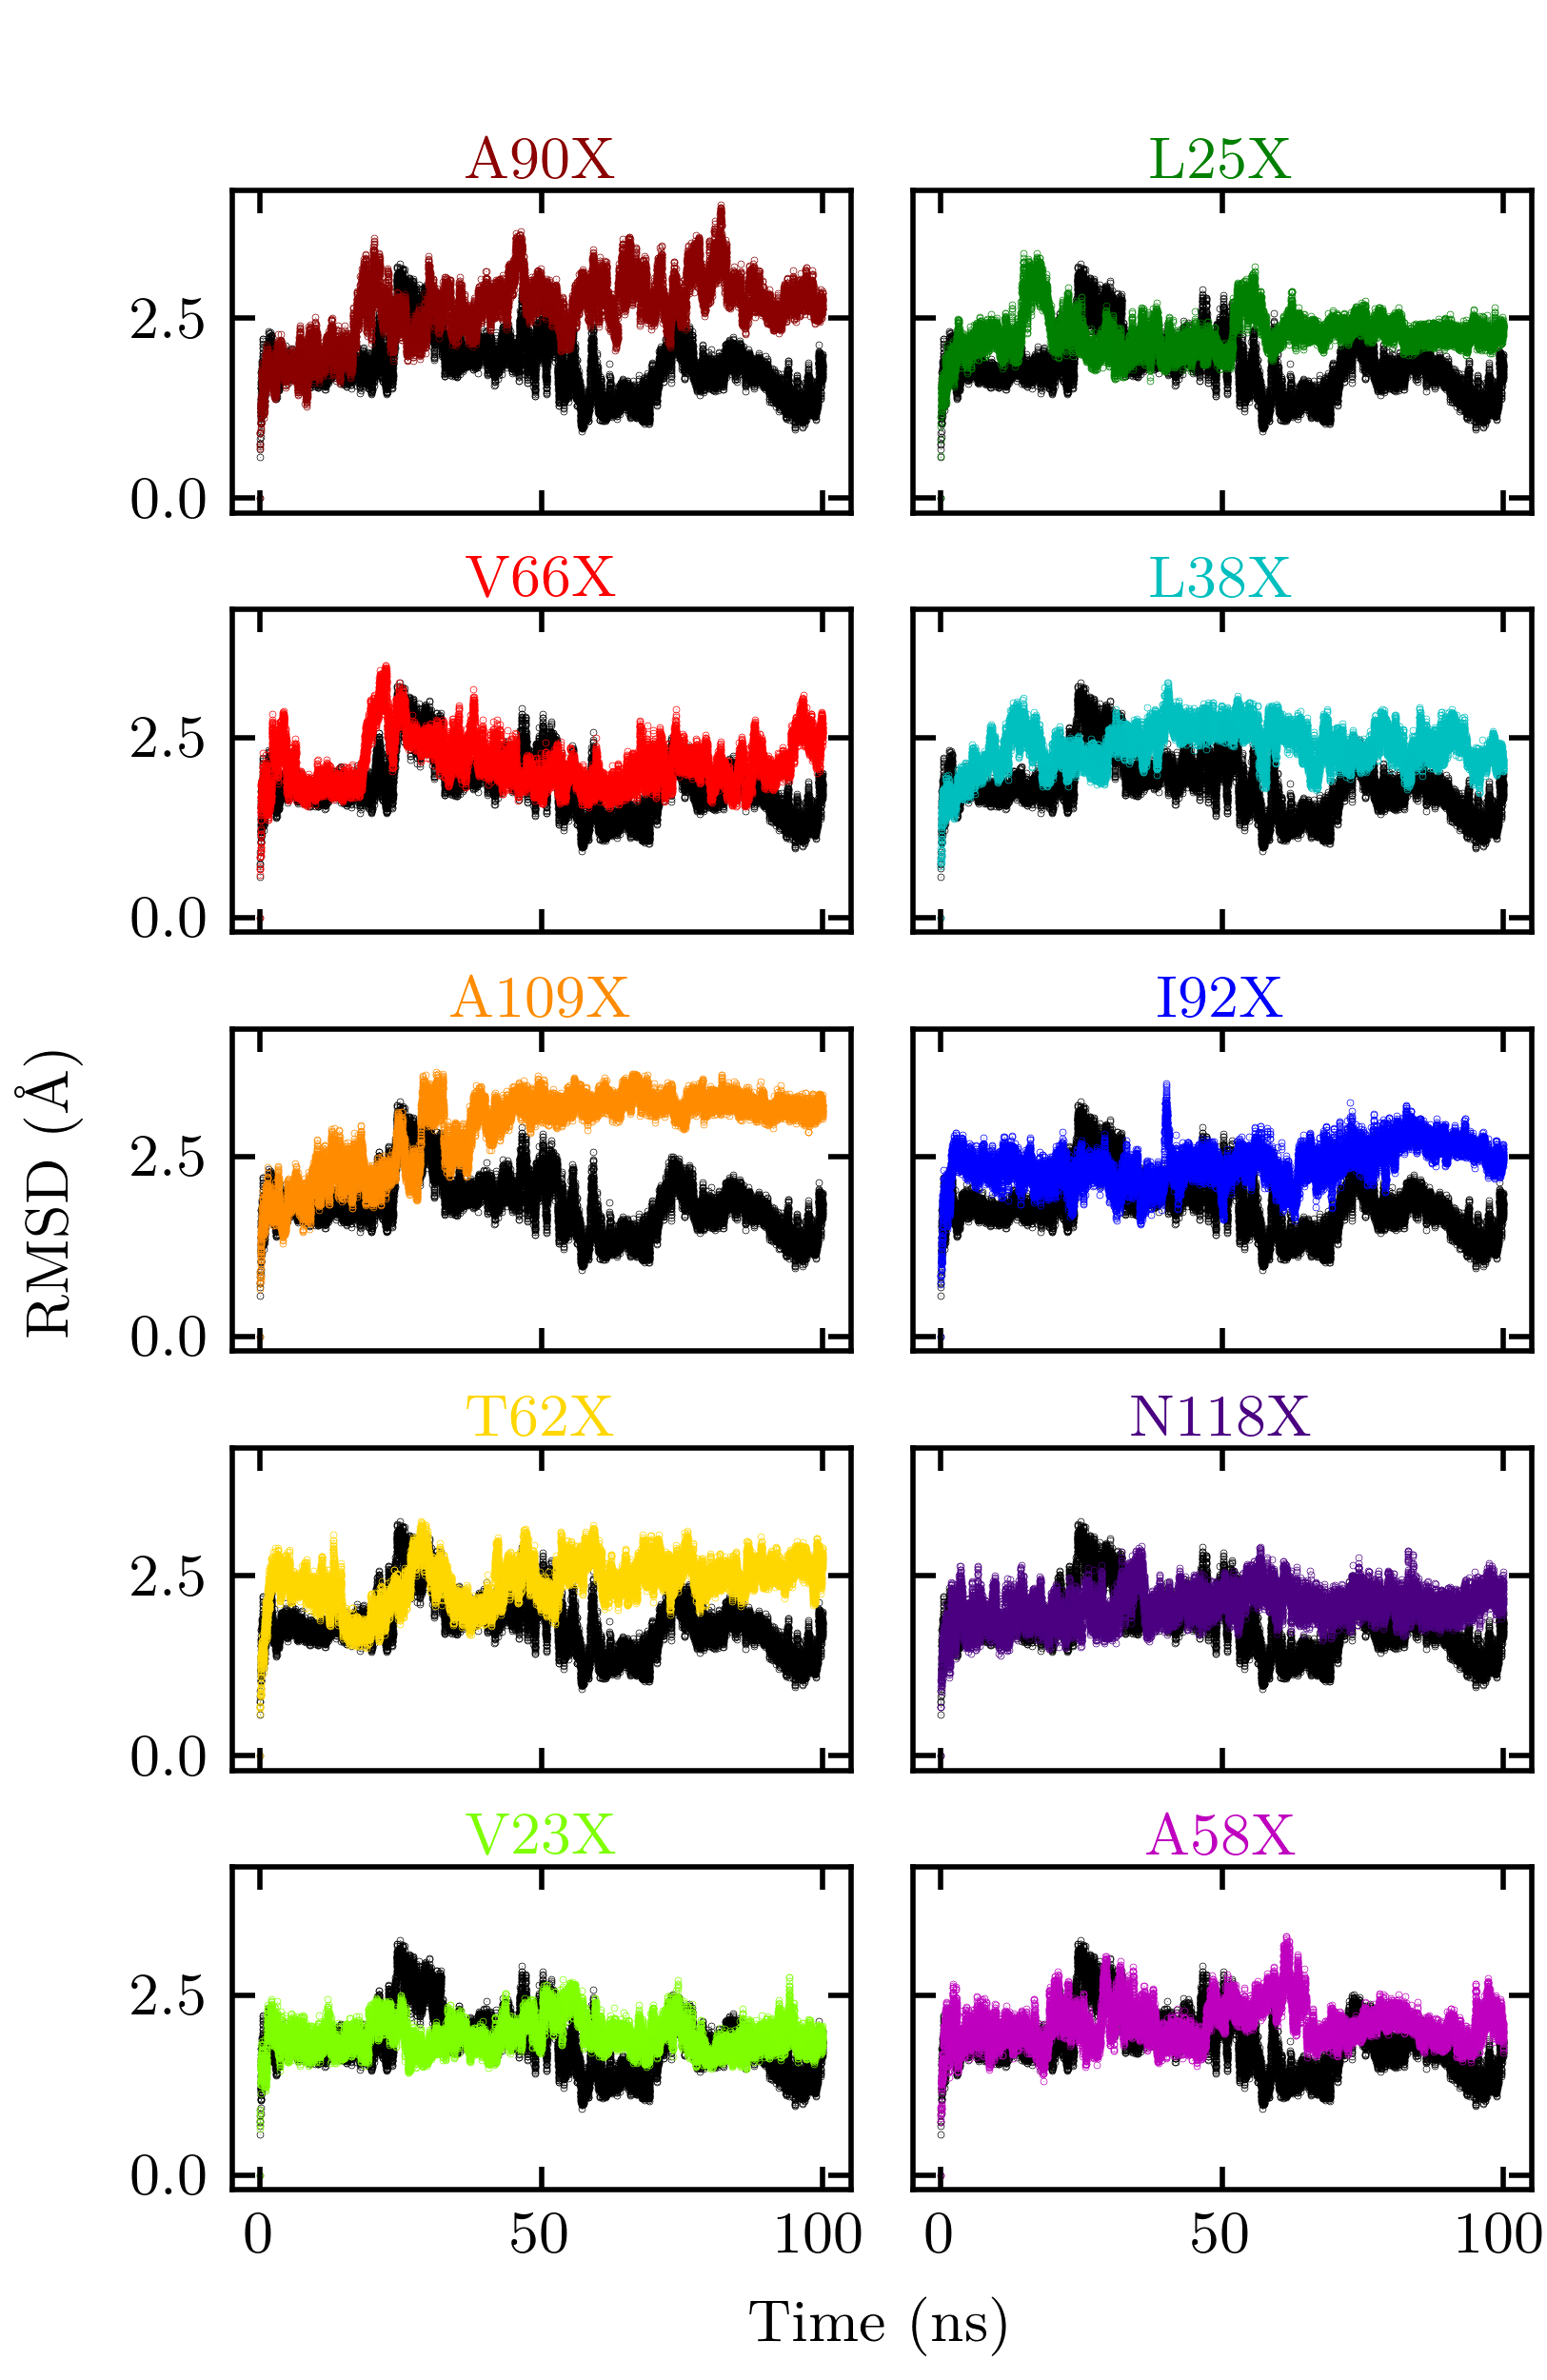
\includegraphics[width=\single]{figures-snase/rmsd.png}
    \caption[Backbobe RMSDs of nitrile containing SNase constructs]{
        Backbone RMSDs of the crystalized residues (residues 7-141) of each nitrile containing SNase constructs (color traces) and the WT SNase (black).
    }
    \label{fig:snase-rmsd}
\end{figure}

Second, we investigated the specific geometries of hydrogen bonding interactions in the MD simulations. 
The geometries were calculated using an in-house code described previously, based on criteria illustrated in Figure \ref{fig:snase-hbond_criteria} \cite{First2018}.
In order to be classified as a hydrogen bond, $d_\text{NH}$ needed to be less than 2.45 \si{\angstrom}, $\theta_1$ needed to be greater than \ang{99}, and $\theta_2$ needed to be greater than \ang{120}. 
Since $\theta_1$ has been shown to have a large impact on the nitrile frequency \cite{Choi2008, First2018}, we plotted $\theta_1$ against $d_\text{NH}$ of each interaction as a heat map in Figure \ref{fig:snase-hbond} considering either only water molecules (Figure \ref{fig:snase-hbond}A) or protein O, N, and C$_{\alpha}$ atoms with a covalently bound hydrogen atom (Figure \ref{fig:snase-hbond}B) to be possible hydrogen bond donors. 
Figure \ref{fig:snase-hbond}A demonstrates that the nitrile locations experienced a wide range of solvent hydrogen-bonding environments. 
The nitriles at positions N118X and A58X had a broad distribution of hydrogen bonding geometries that were donated from water molecules, consistent with partially solvent-exposed residues or interaction with unstructured water. 
I92X and V66X experienced far fewer hydrogen bonds to solvent (less than 1,500 occurrences each out of 25,000 frames analyzed) that were also broadly distributed around the measured geometries. 
This indicated a low level of interaction with unstructured water. A90X, L25X, A109X, V23X and L38X experienced few hydrogen bonds to solvent (less than 600 occurrences each). 
Finally, T62X experienced a significant amount of hydrogen bonding to solvent (over 17,000 occurrences) with a narrow distribution of $\theta_1$. 
Upon inspection, this population was found to result from a structural water that was stabilized by hydrogen bonding to the amide N atoms of both Ile18 and Asp19 and to the carboxyl O of Thr22. 
The water molecule in this interaction was found to be extremely stable and exchanged very infrequently. 
For example, one instance of a water molecule in this location had a residence time of over 40 ns. 
To visualize this, we plotted the number of hydrogen bonds that persisted for at least that length of time as a function of simulation time (Figure \ref{fig:snase-lifetimes}). 
The residence time of the water molecules in this interaction with T62X was significantly longer than any other interaction observed in any of our simulations.

\begin{figure}
    \center
    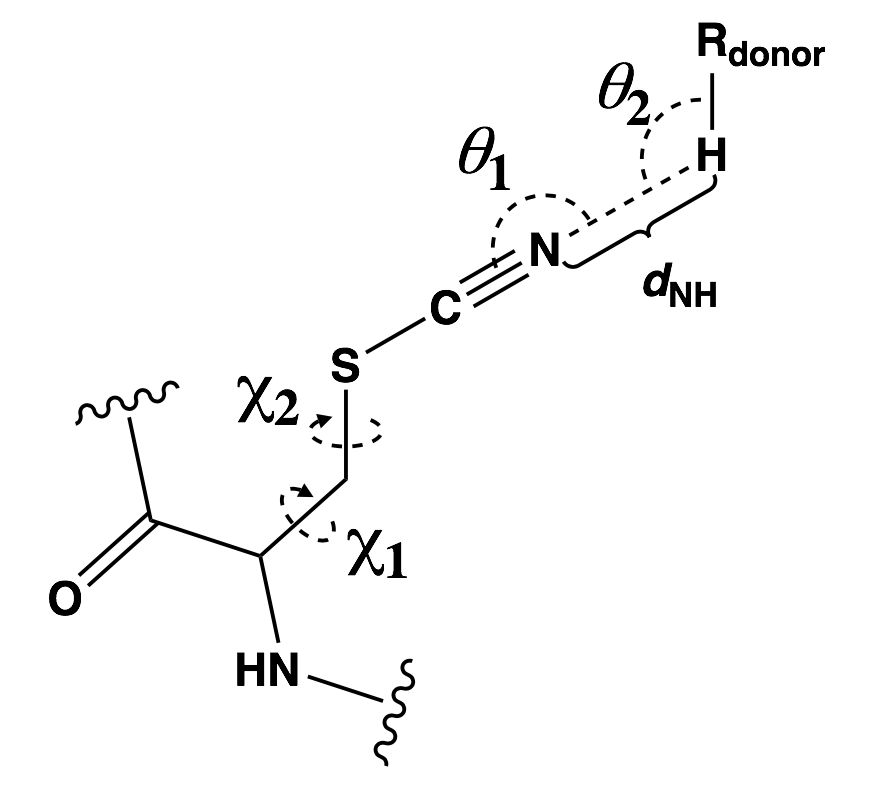
\includegraphics[width=\single]{figures-snase/hbond_schematic.png}
    \caption[Schematic of the hydrogen bonding geometric criteria]{
        Schematic of the hydrogen bonding geometric criteria. 
        $\theta_1$ is the C$\equiv$N$\cdots$H angle. 
        $\theta_2$ is the N$\cdots$H-R$_\text{donor}$ angle, where R$_\text{donor}$ represents any hydrogen bond donor. 
        $d_\text{NH}$ is the distance between the hydrogen and the acceptor nitrogen. 
        In this analysis, any S, N, O, or C$_{\alpha}$ atom was considered to be a potential hydrogen bond donor. 
        To be considered a hydrogen bond, $\theta_1$must be greater than \ang{99}, $\theta_2$ must be greater than \ang{120}, and  $d_\text{NH}$ must be less than 2.45 \si{\angstrom}.
    }
    \label{fig:snase-hbond_criteria}
\end{figure}

\begin{figure}
    \center
    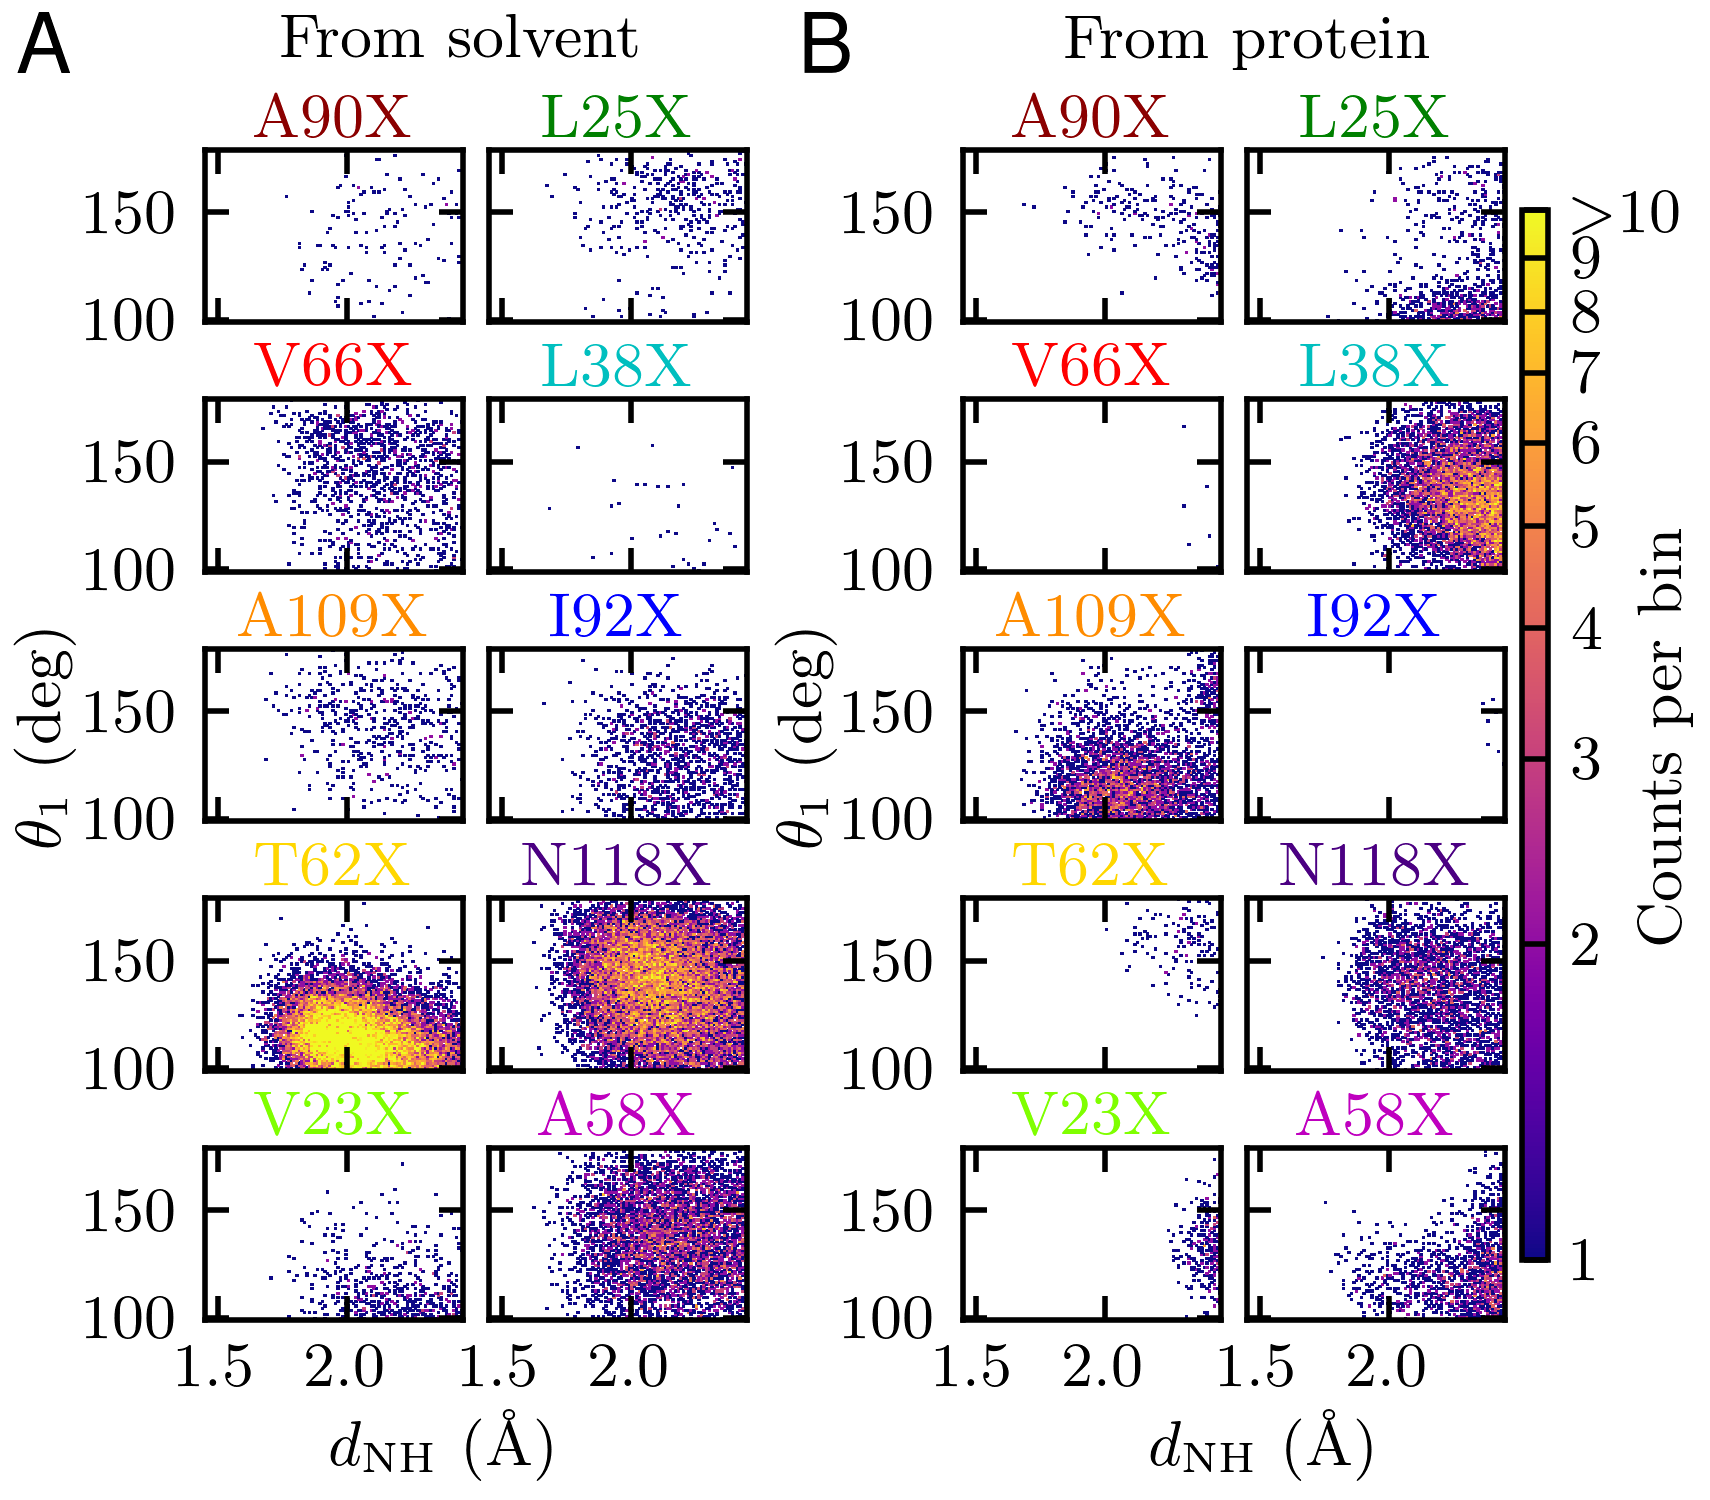
\includegraphics[width=\single]{figures-snase/Geometry_combined.png}
    \caption[Heat maps of hydrogen bonding geometries to CNC at each probe location]{
        Heat maps of hydrogen bonding geometries to CNC at each probe location. 
        (A) Hydrogen bonds that are donated specifically from water. 
        (B) Hydrogen bonds that are donated from the protein.
    }
    \label{fig:snase-hbond}
\end{figure}

\begin{figure}
    \center
    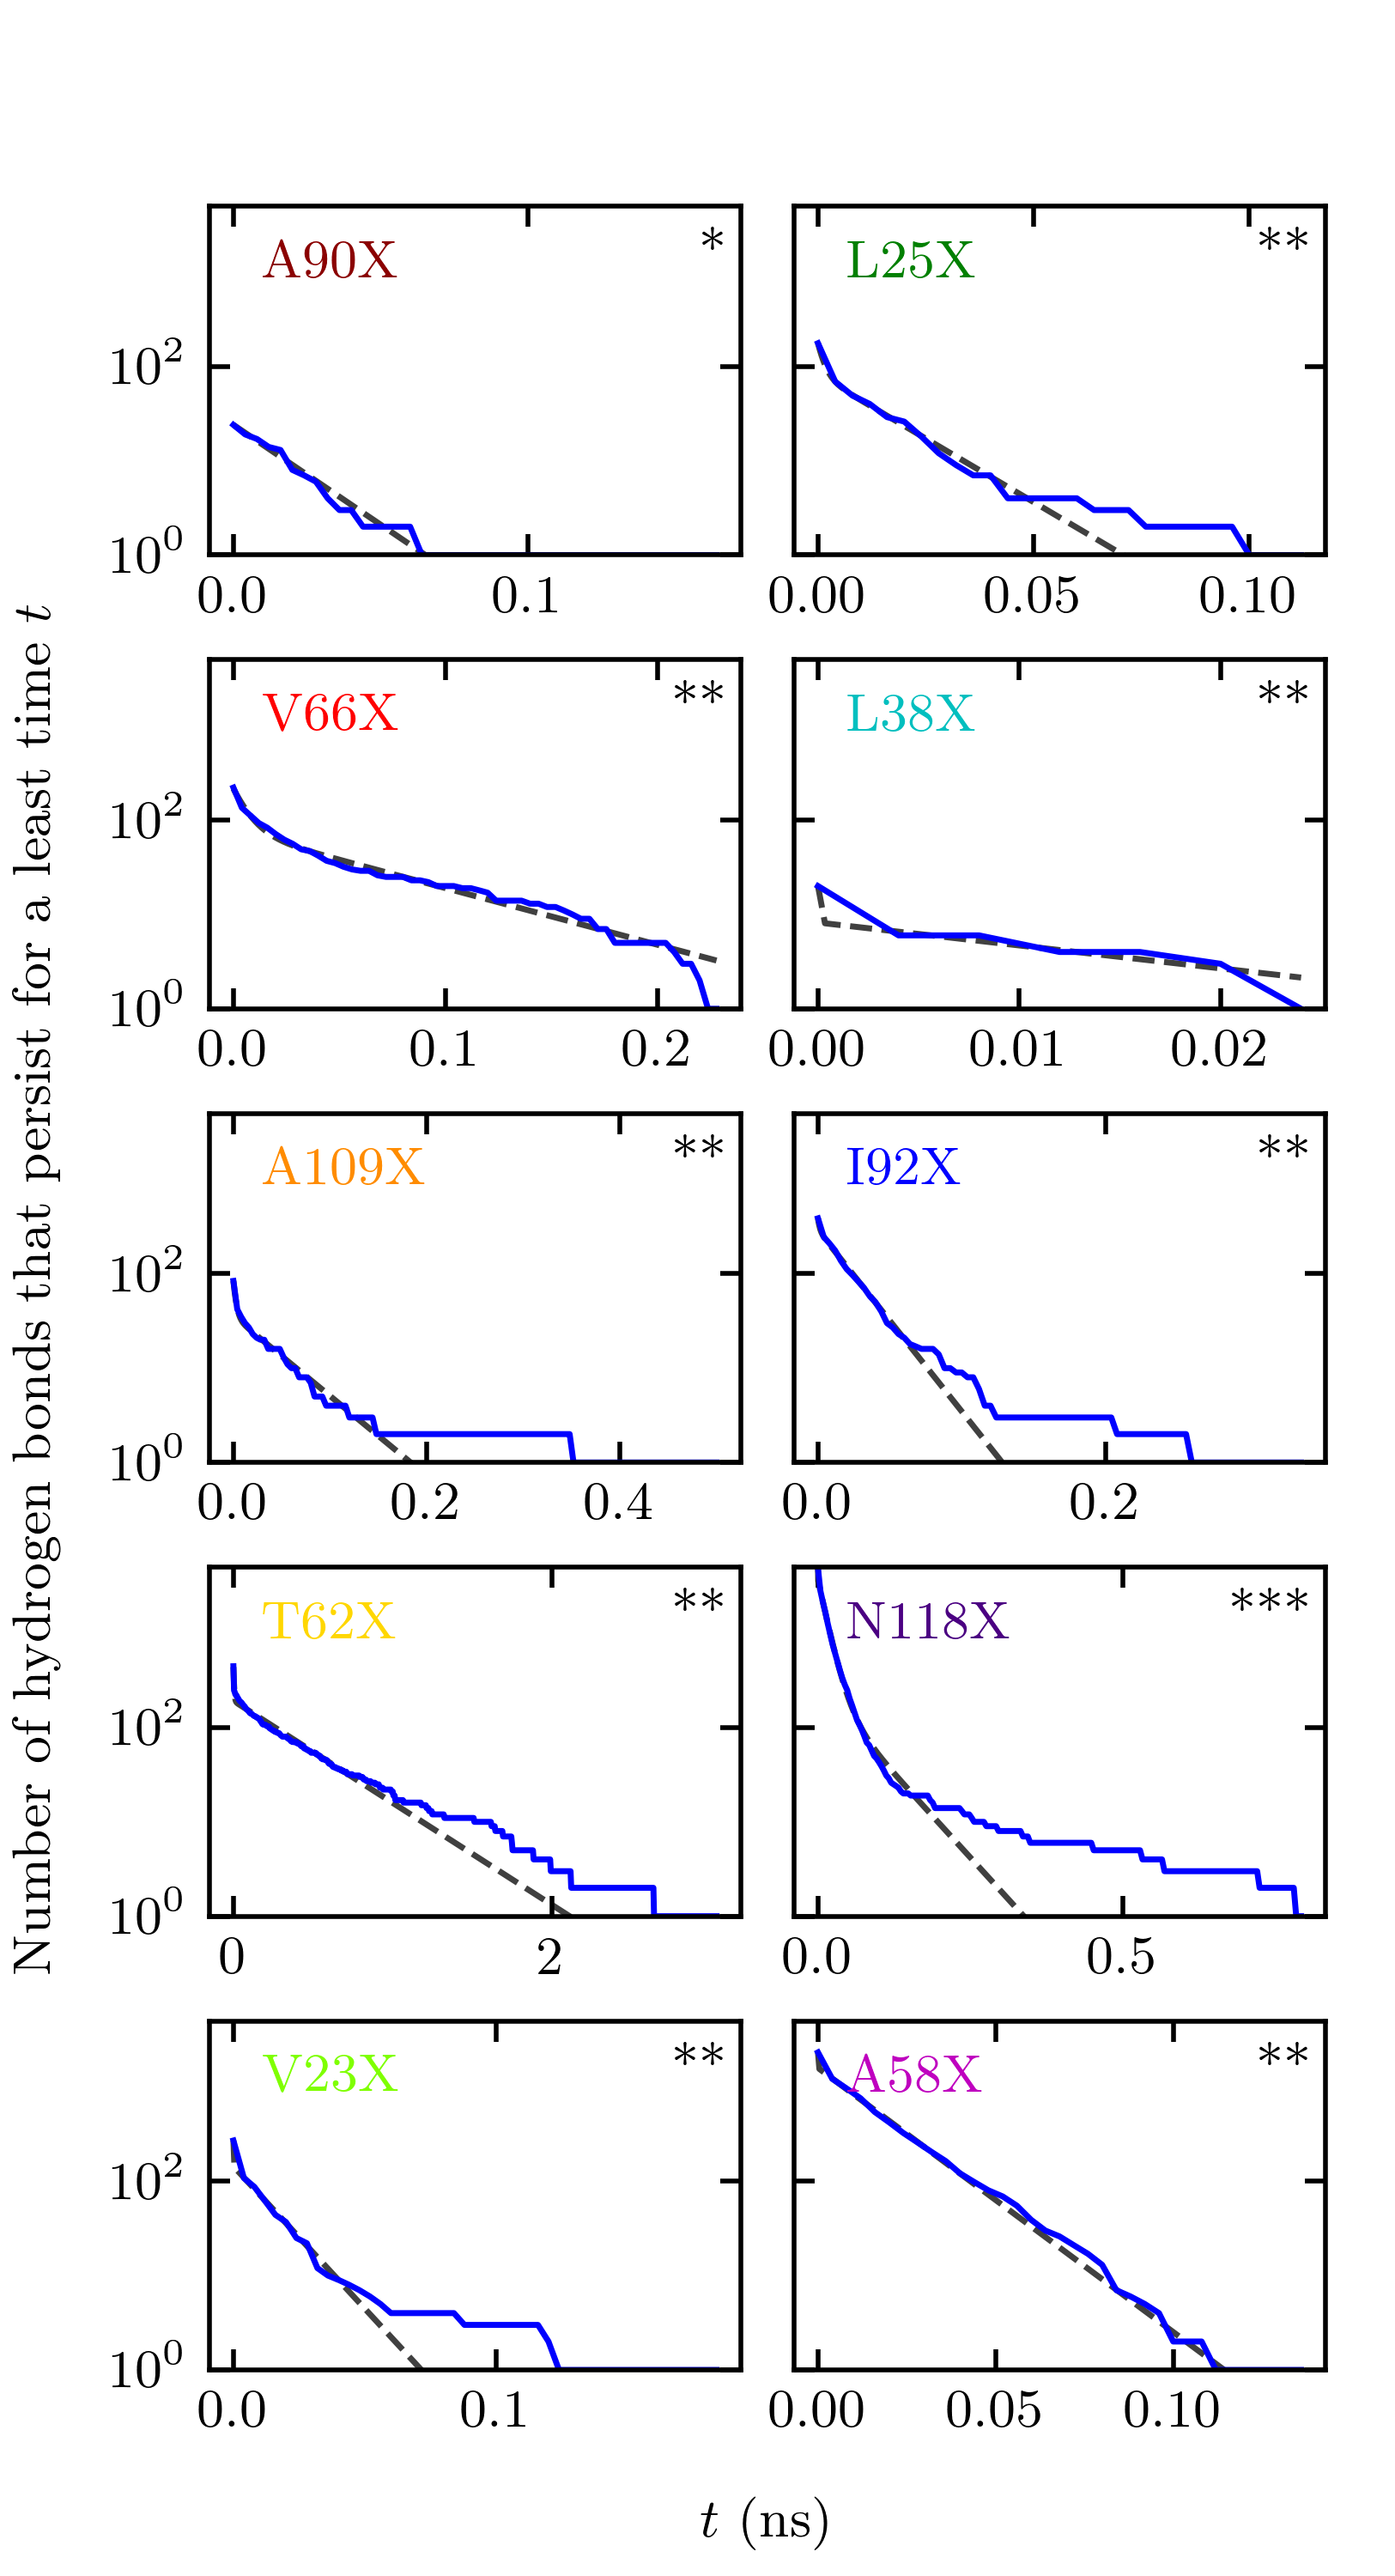
\includegraphics[width=\single]{figures-snase/Lifetimes.png}
    \caption[]{
        Calculation of the observed hydrogen bond residence times for the nitrile at each location. 
        The $y$-axis is the number of hydrogen bonds observed that lasted at least as long as the simulation time shown on the $x$-axis. 
        The dashed line represents a fit of a single, double, or triple exponential decay where the number of decay function is indicated by the number of asterisks in the top right corner of each plot. 
        Note the difference in scale of the $x$-axes.
    }
    \label{fig:snase-lifetimes}
\end{figure}

Likewise, the nitriles experienced a range of hydrogen bonding interactions from nearby protein donors (Figure \ref{fig:snase-hbond}B). 
The nitriles at positions L38X, A109X, and N118X experienced a significant amount of hydrogen bonding (over 3,000 observations) from nearby protein donors. 
The nitrile at positions A58X and L25X experienced a small amount of hydrogen bonding from protein (less than 1,700 occurrences). 
The nitriles at positions V23X, A90X, V66X, I92X, and T62X experienced almost no hydrogen bonding interactions from protein (less than 400 occurrences each). 
It is important to note that in all probe locations, the nitrile was observed to be involved in some amount of hydrogen bonding interaction, either with water or with the protein itself. 
This is likely true for \pKa{} probes in these same positions because crystal structures of SNase with \pKa{} probes at these locations show likely hydrogen bonding between the probe and nearby residues or crystallized water \cite{Robinson2018}. 
Taken together, these data demonstrate that with both \pKa{} and nitrile probes, hydrogen bonding interactions cannot be assumed to be absent or even consistent between probe locations. 
The local interactions at each location must be understood to interpret experimental results.

Despite the nitriles being buried in the hydrophobic core of SNase, our MD simulations revealed a spectrum of hydrogen bonding interactions, consistent with our observations of a range of FWHMs of the spectra in Figure \ref{fig:snase-ftir}. 
Beyond this, the two nitriles with spectra that had the largest FWHM, N118X and A58X, experienced a broad range of hydrogen bonding geometries in our simulations, consistent with solvent exposure. 
Conversely, the nitriles with the narrowest spectra, V66X, V23X, A90X, I92X, and L25X, all experienced relatively few hydrogen bonds in our simulations. 
Finally, nitriles with intermediate spectral widths, A109X, L38X, and T62X, all experienced structural hydrogen bonds. 
The hydrogen bonds to A109X and L38X were donated by protein, and the vast majority of hydrogen bonding events to T62X were from a structurally rigid water molecule. 
The apparent correlation of observed hydrogen bonding in simulation and the experimentally measured FHWMs suggests that hydrogen bond exchange was a significant source of heterogeneity for the nitrile probes in our system. 
Further, because these locations were chosen intentionally to be buried in the hydrophobic core of a globular protein, it may be impossible to position a nitrile probe site-specifically in a protein location completely void of hydrogen bonding. 
This is consistent with our previous work in GFP, in which every nitrile positioned in a wide range of environments experienced hydrogen bonding \cite{First2018}. 
Even in the buried hydrophobic core of a protein, such as in this case with SNase, one cannot assume a nitrile probe is free from hydrogen bonding, and in all systems, controls must be performed to account for these interactions. 
This is not unique to vibrational probes; 
the inclusion of any molecular probe, including a \pKa{} probe, requires careful consideration of local interactions that are difficult to predict \emph{a priori}. 

To investigate the effect of these local interactions on our observed vibrational spectra, we calculated the most probable C$\equiv$N$\cdots$H hydrogen bonding angle ($\theta_1$ in Figure \ref{fig:snase-hbond_criteria}), as described previously, and compared this angle to the observed vibrational frequencies. 
Because some of the nitrile locations in SNase experienced relatively few hydrogen bonding interactions, we weighted the regression based on the number of hydrogen bond observations to each nitrile. 
The most probable $\theta_1$ was well-correlated to the observed vibrational frequency of the nitrile (Figure \ref{fig:snase-theta_vs_freq}, $r = 0.72$). 
This is consistent with \emph{ab initio} calculations by Choi et al., where linear, \textsigma-hydrogen bonds ($\theta_1$ closer to \ang{180}) were shown to blue shift the nitrile frequency and non-linear, \textpi-hydrogen bonds ($\theta_1$ closer to \ang{120}) were shown to red shift the nitrile frequency \cite{Choi2008, First2018}. 
Thus, we have demonstrated that 
1) it may impossible to position a nitrile in a location free from hydrogen bonding in a biological molecule and 
2) any interpretation of nitrile frequencies must take the specific geometry of hydrogen bonding into consideration in order to interpret the observed results.

\begin{figure}
    \center
    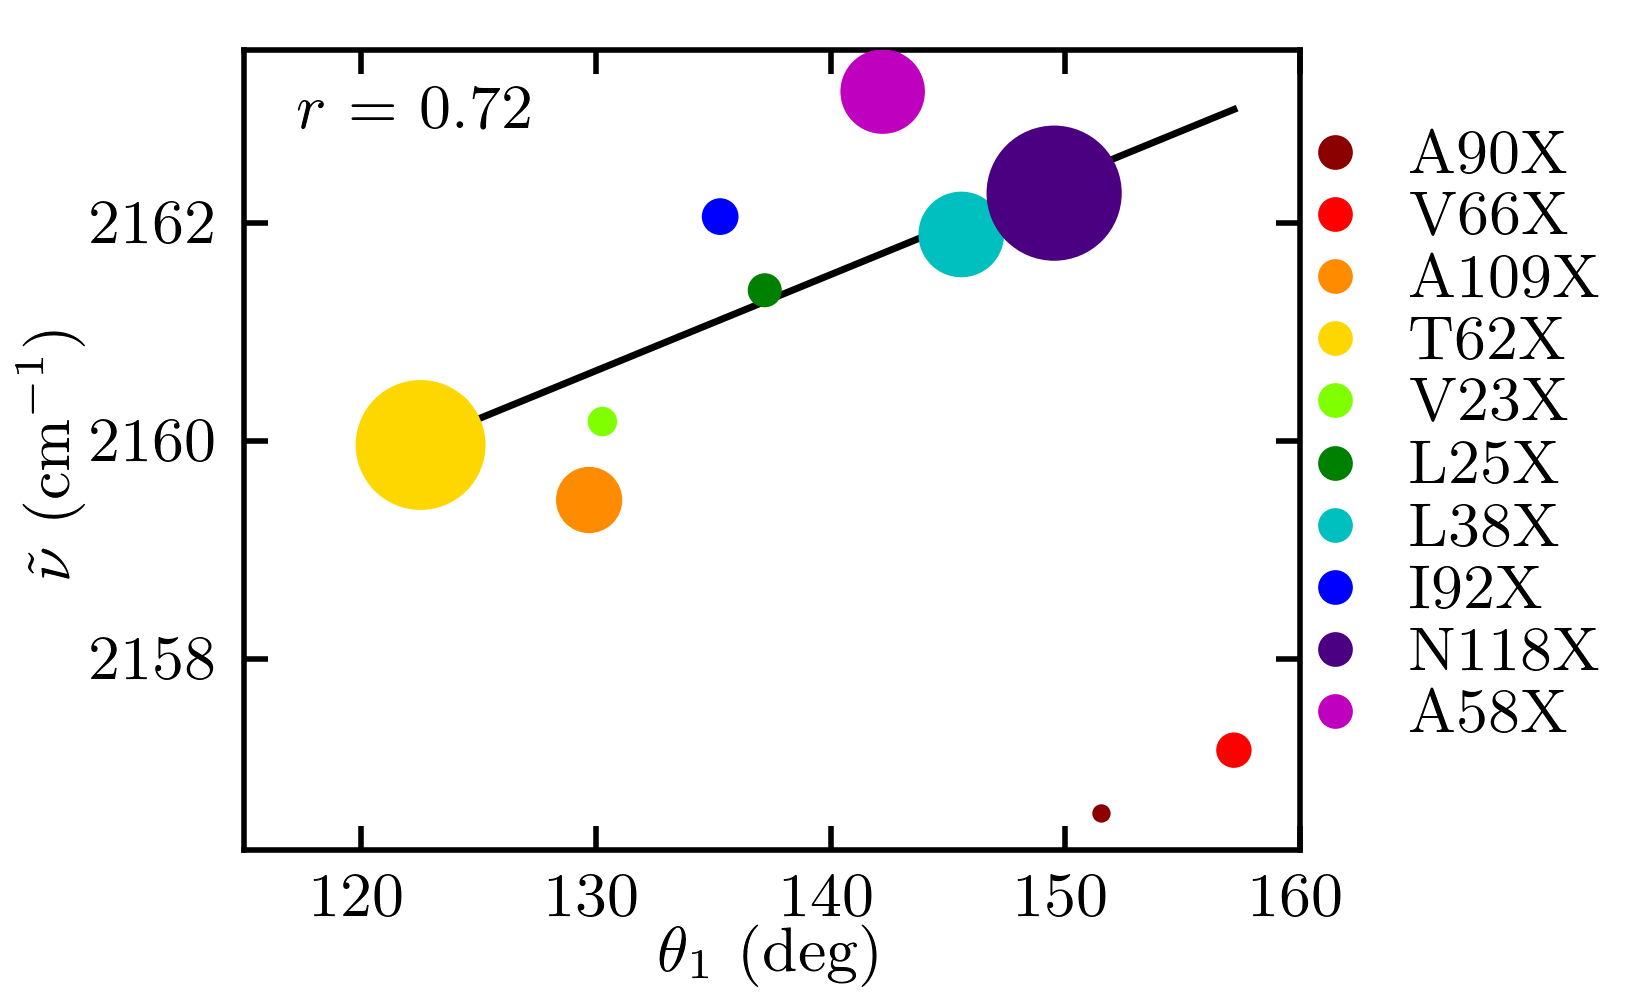
\includegraphics[width=\single]{figures-snase/weighted_abs_max_vs_max_theta.png}
    \caption[The most probable angle of hydrogen bonding against the experimental vibrational frequency]{
        The most probable angle of hydrogen bonding from simulation is plotted against the experimental peak vibrational frequency for each of the 10 nitrile locations in SNase. 
        The most probable angle was calculated as described previously \cite{First2018}. 
        All vibrational frequencies shown here were measured at room temperature. 
    }
    \label{fig:snase-theta_vs_freq}
\end{figure}

\subsection{FTLS is a quantitative measure of hydrogen bonding interactions to nitriles}

In order to investigate the hydrogen-bonding environments of the different probe locations experimentally, we measured the FTLS of the nitrile probe in each location. 
Adhikary et al. postulated an empirical relationship between the ability of a nitrile probe to accept a hydrogen bond and the dependence of the nitrile frequency on changes in temperature \cite{Adhikary2015}. 
This is due to an increase in hydrogen bond exchange and accompanying decrease in hydrogen bond lifetime with increasing temperature. 
In systems with fewer hydrogen bonds to the nitrile, less exchange is observed and the resulting temperature dependence of the frequency shift, quantified as the FTLS, is smaller. 
We measured the nitrile absorption frequency of each probe at 10 \si{\celsius} intervals from 5 \si{\celsius} to 35 \si{\celsius}. 
The $\Delta+$PHS construct of SNase was designed to be exceptionally thermally stable \cite{Isom2010, Byrne1995, Garcia-Moreno1997}, and representative CD spectra shown in Figure \ref{fig:snase-cd} demonstrate that the fold of the protein at 35 \si{\celsius} does not change upon heating. 
As expected, the change in vibrational frequency at each location over the temperature range was linear (Figure \ref{fig:snase-ftls}), and the slope of this linear dependence was taken to be the FTLS of each nitrile probe (Table \ref{tbl:snase-ftir}). 
For reference, we also plotted the temperature dependent frequency shift of MeSCN in both \ce{H2O} and DMSO in Figure \ref{fig:snase-ftls}, which allowed us to compare the measured FTLS of the nitriles in protein to the amount of hydrogen bonding a nitrile experiences in protic and aprotic environments, respectively.

\begin{figure}
    \center
    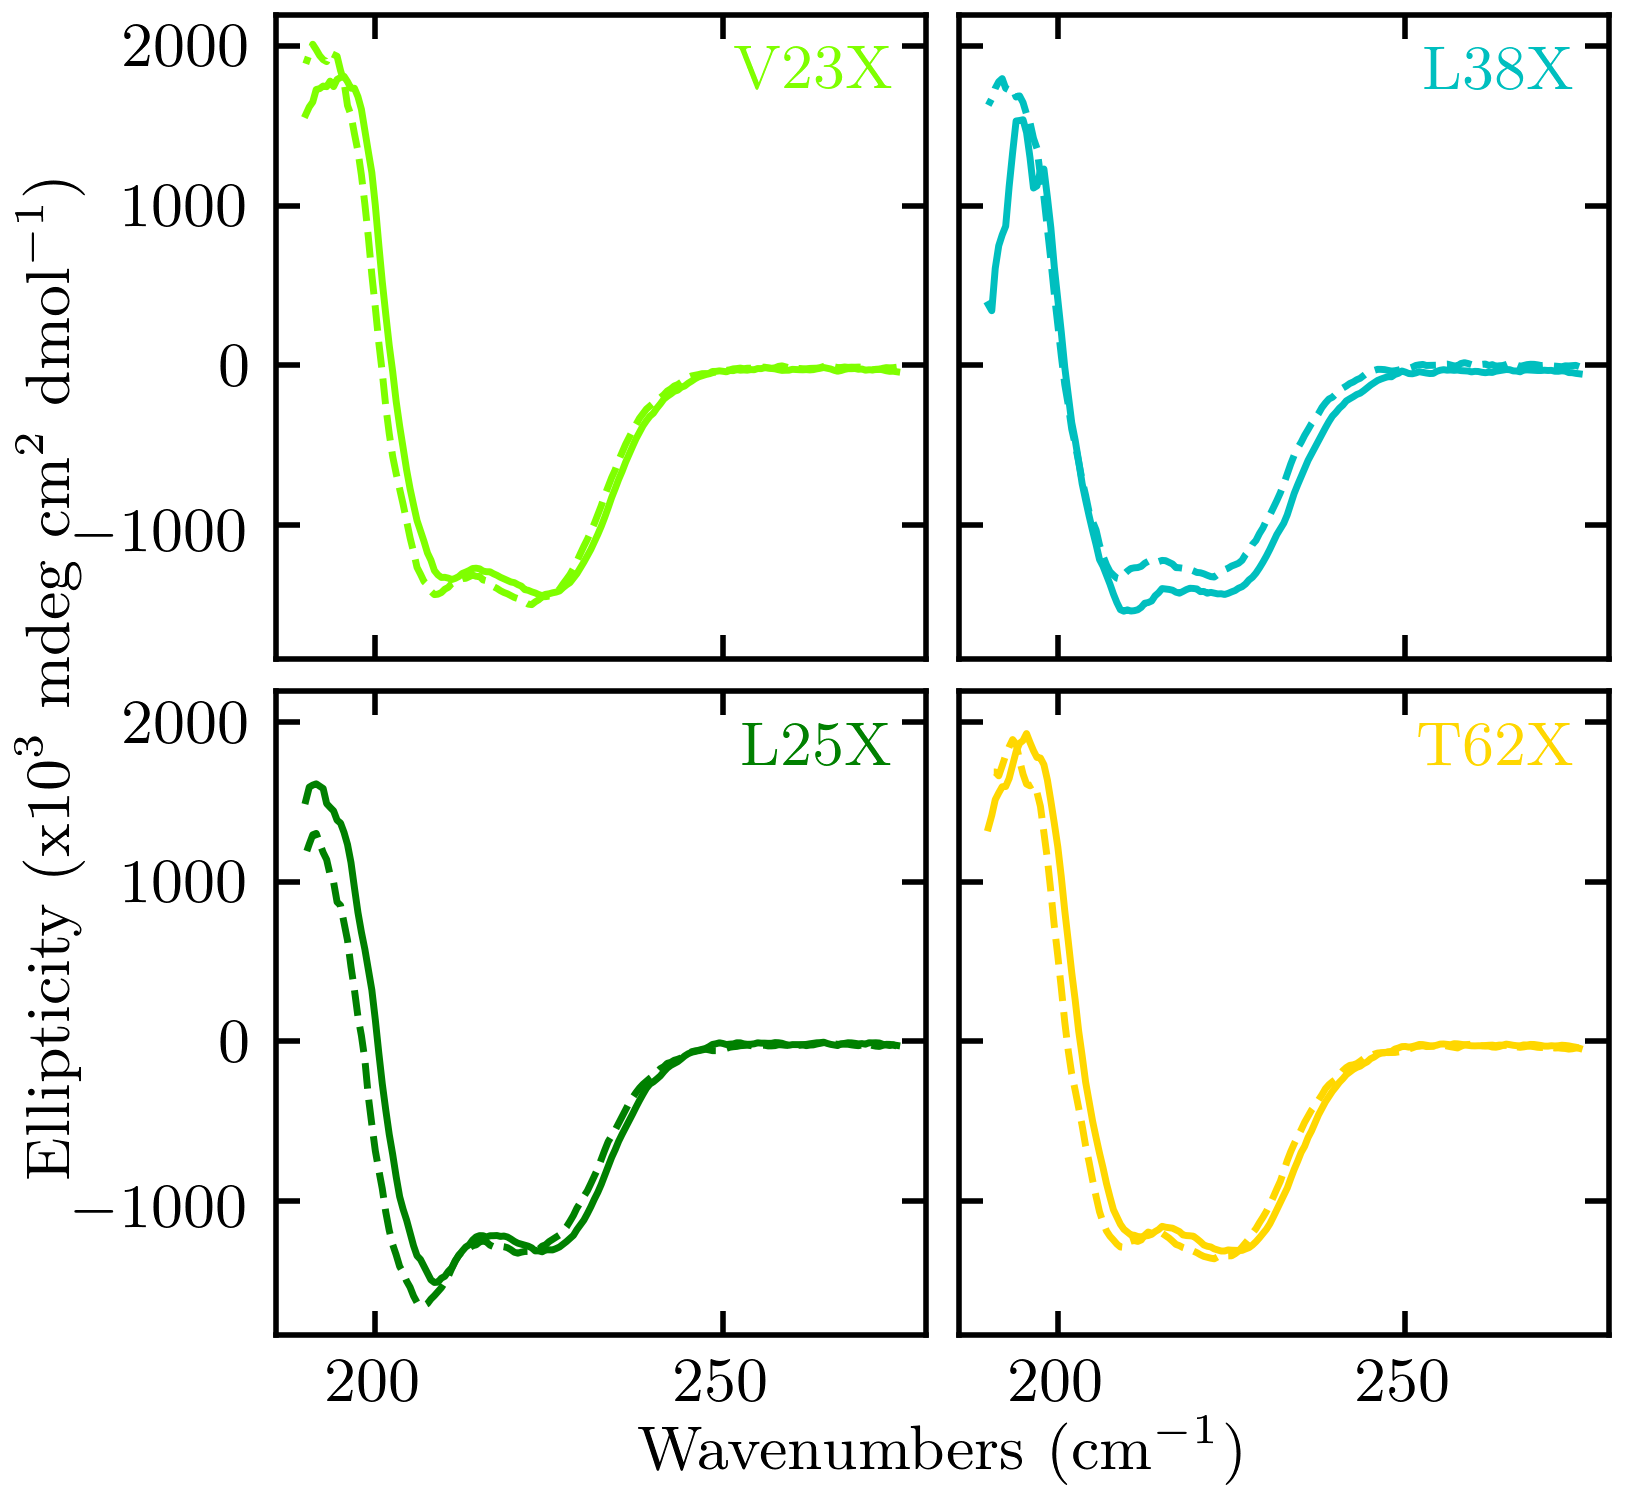
\includegraphics[width=\single]{figures-snase/cd_spectra.png}
    \caption[Representative CD spectra of mutants at room temperature and at 35 \si{\celsius}]{
        Four representative CD spectra of mutants at room temperature (solid lines) and at 35 \si{\celsius} (dashed lines). 
        Reported spectra are the average of at least 5 scans.
    }
    \label{fig:snase-cd}
\end{figure}

\begin{figure}
    \center
    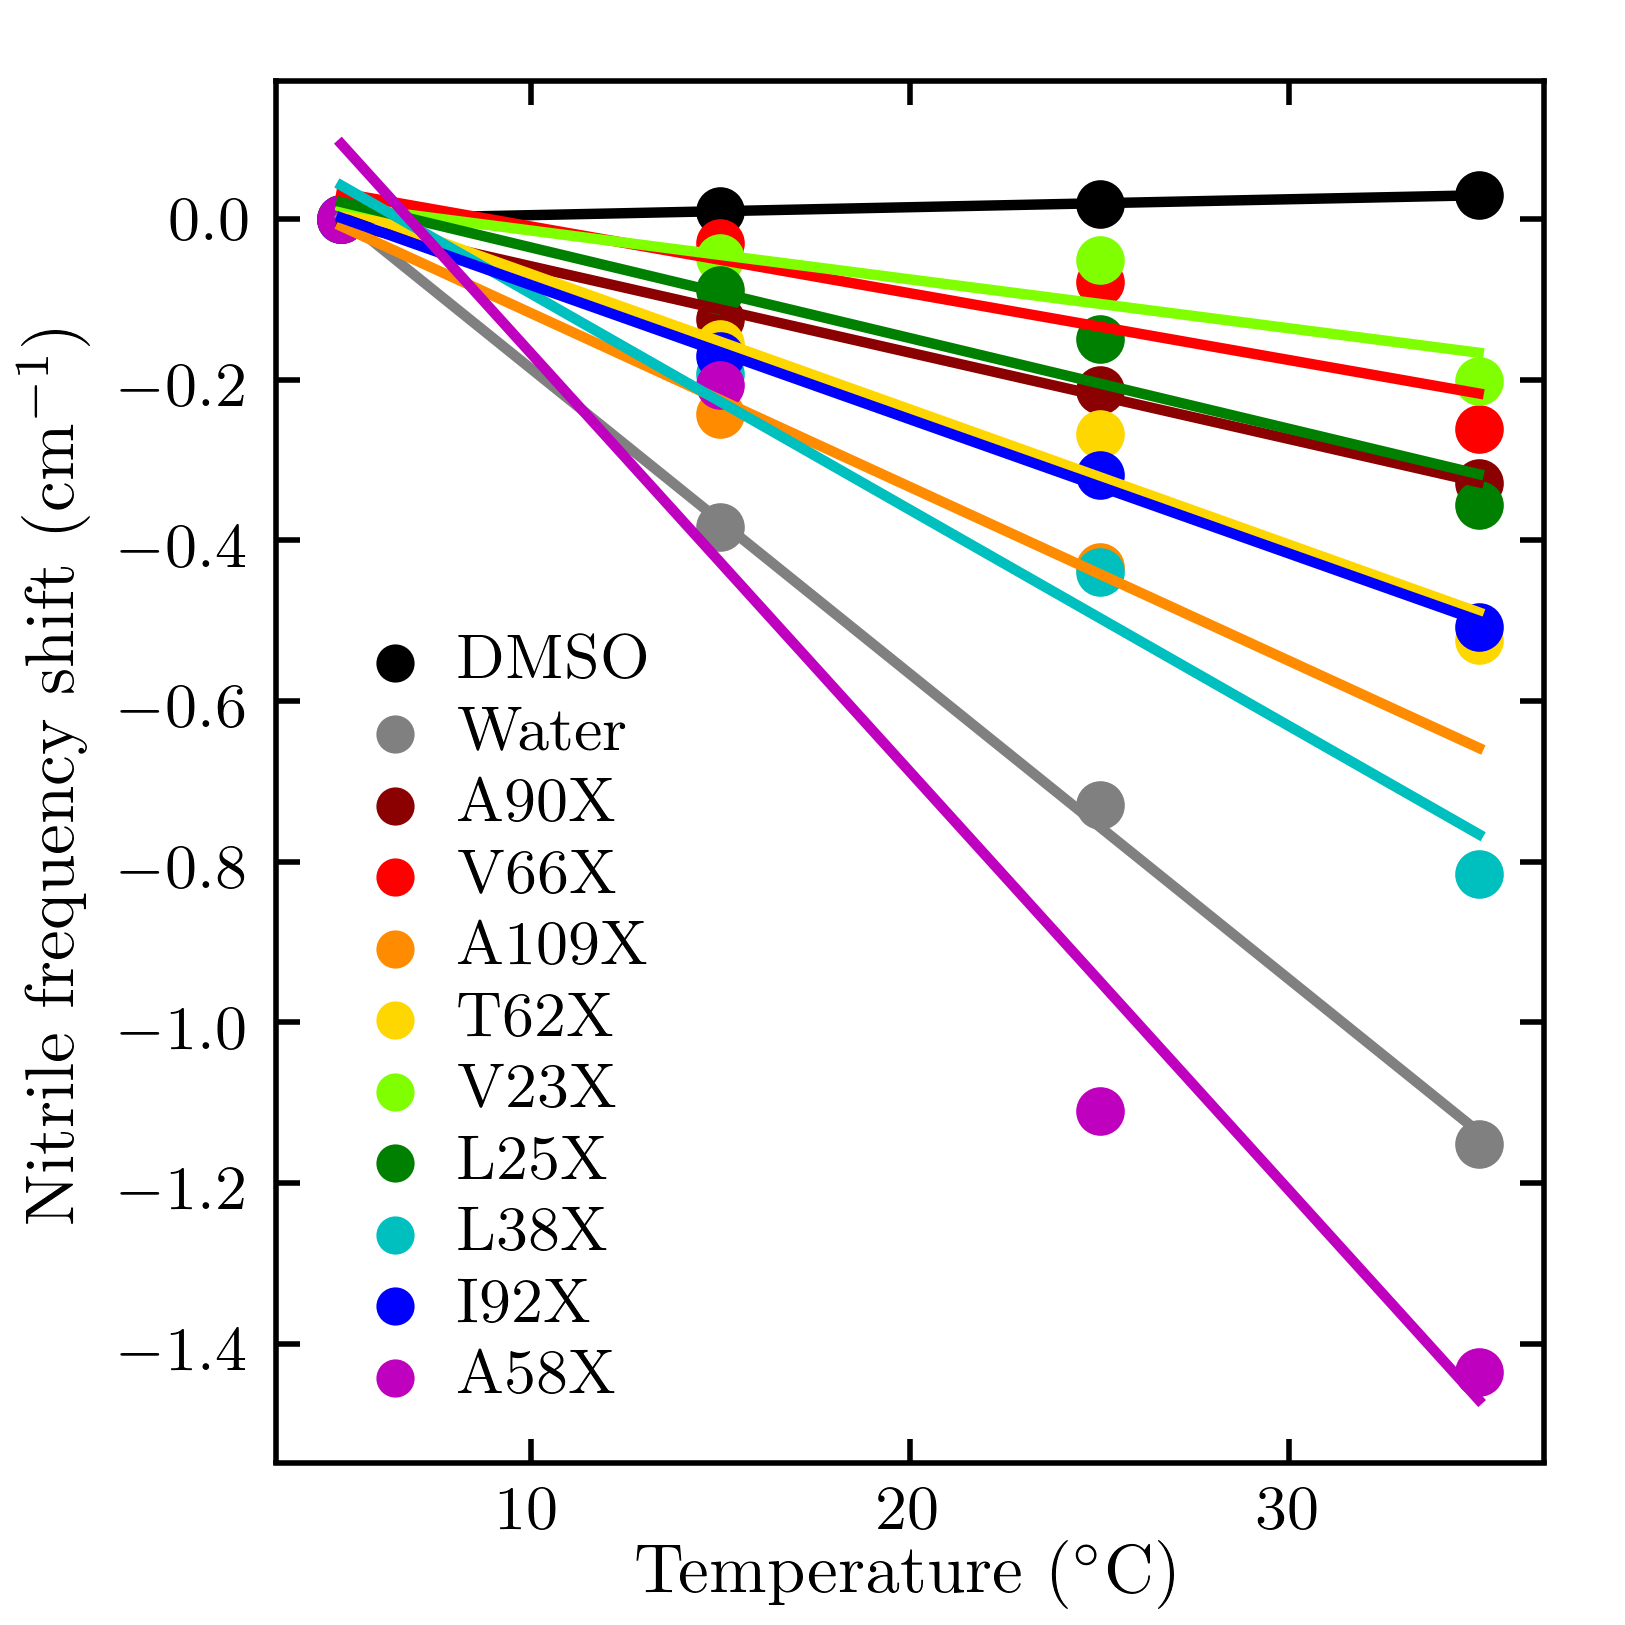
\includegraphics[width=\single]{figures-snase/ftls.png}
    \caption[]{
        Average of peak nitrile frequencies of the 10 nitrile probes from 5 \si{\celsius} to 35 \si{\celsius}. 
        The points for each mutant were fit to a linear regression. 
        The slopes and the standard error of the fits are given in Table \ref{tbl:snase-ftir}.  
        Mutants are colored according to Figure \ref{fig:snase-system}. 
        Mean nitrile frequencies of MeSCN in DMSO and water at the same temperatures are also shown in black and gray, respectively. 
        Error bars were excluded for clarity but are listed in Table \ref{tbl:snase-ftls}. 
        No data was collected for MeSCN in DMSO at 5 \si{\celsius} because it is below the freezing point of DMSO.
    }
    \label{fig:snase-ftls}
\end{figure}

\begin{table}
    \caption[Peak vibrational frequencies at a range of temperatures]{
        Peak vibrational frequencies of nitrile probes at each location at a range of temperatures.
    }
    \begin{center}
        \resizebox{\double}{!}{
    \begin{tabular}{c|c|c|c|c}
    \toprule
    \multirow{2}{*}[-2pt]{CNC location} &   \multicolumn{4}{c}{Average peak vibrational frequency (\si{\wn})} \\
\cmidrule[0.2pt](){2-5}
     & 5 \si{\celsius} & 15 \si{\celsius} & 25 \si{\celsius} & 35 \si{\celsius} \\
    \midrule
    A90X   &  $2156.93    \pm 0.01   $ &   $2156.83    \pm 0.02   $ &  $2156.72    \pm 0.02   $ &  $2156.62    \pm 0.04   $ \\
    V66X   &  $2157.27    \pm 0.11   $ &   $2157.20    \pm 0.07   $ &  $2157.15    \pm 0.04   $ &  $2157.08    \pm 0.04   $ \\
    A109X  &  $2160.34    \pm 0.47   $ &   $2160.10    \pm 0.41   $ &  $2159.91    \pm 0.48   $ &  $2159.80    \pm 0.50   $ \\
    T62X   &  $2160.27    \pm 0.08   $ &   $2160.17    \pm 0.08   $ &  $2160.02    \pm 0.07   $ &  $2159.86    \pm 0.05   $ \\
    V23X   &  $2160.35    \pm 0.05   $ &   $2160.28    \pm 0.05   $ &  $2160.22    \pm 0.13   $ &  $2160.12    \pm 0.14   $ \\
    L25X   &  $2161.47    \pm 0.13   $ &   $2161.42    \pm 0.10   $ &  $2161.32    \pm 0.13   $ &  $2161.24    \pm 0.14   $ \\
    L38X   &  $2162.53    \pm 0.13   $ &   $2162.26    \pm 0.09   $ &  $2162.06    \pm 0.02   $ &  $2161.70    \pm 0.18   $ \\
    I92X   &  $2162.32    \pm 0.05   $ &   $2162.18    \pm 0.02   $ &  $2162.04    \pm 0.04   $ &  $2161.83    \pm 0.03   $ \\
    N118X  &  $2164.16    \pm 0.40   $ &   $2163.85    \pm 0.61   $ &  $2163.07    \pm 0.32   $ &  $2162.66    \pm 0.36   $ \\
    A58X   &  $2163.80    \pm 0.30   $ &   $2163.55    \pm 0.27   $ &  $2163.28    \pm 0.40   $ &  $2162.98    \pm 0.36   $ \\
    DMSO$^a$& $  --                  $ &   $2153.52    \pm 0.04   $ &  $2153.51    \pm 0.01   $ &  $2153.35    \pm 0.03   $ \\
    Water  &  $2163.58    \pm 0.02   $ &   $2163.15    \pm 0.01   $ &  $2162.66    \pm 0.17   $ &  $2162.33    \pm 0.01   $ \\
    \bottomrule
    \end{tabular}
}
    \end{center}
    $^a$No data was collected for MeSCN in DMSO at 5 \si{\celsius} because it is below the freezing point of DMSO.
    \label{tbl:snase-ftls}
\end{table}

The ten nitrile-containing SNase constructs demonstrated a large range of FTLS. 
V66X, V23X, L25X, and A90X all had small FTLS of -0.006, -0.008,  0.008, -0.011 \si{\wn} \si{\celsius}$^{-1}$, respectively. 
T62X, I92X, and A109X had moderate FTLS of -0.014, -0.016, and -0.018 \si{\wn} \si{\celsius}$^{-1}$, respectively. 
For the nitriles at positions L38X and A58X, the FTLS were larger, both at  0.027 \si{\wn} \si{\celsius}$^{-1}$. 
Finally, the nitrile at position N118X ( 0.053 \si{\wn} \si{\celsius}$^{-1}$) had FTLS that was larger than that of water (-0.043 \si{\wn} \si{\celsius}$^{-1}$), indicating a larger temperature response by the probe than MeSCN in water. 
At this position, the probe was located in a flexible portion of the protein, which we hypothesize can sample more environments as temperature increases. 
This increased flexibility results in a larger temperature dependence than a small molecule nitrile in water. 

In order to investigate whether the FTLS measurements accurately served as a measure of hydrogen bonding according the relationship postulated by Adhikary et al.\cite{Adhikary2015}, we compared the FTLS to the amount of hydrogen bonding to the nitrile observed in our MD simulations. 
To this end, we first calculated the solvent accessible surface area (SASA) of the nitrile-containing residue (Figure \ref{fig:snase-sasa}), as this is often used as a first approximation of hydrogen bonding access. 
While residues such as N118X had larger SASA values, most nitriles had a small calculated SASA with relatively large fluctuations. 
These fluctuations led to standard deviations that were larger than the differences in the averages, despite the evidence that nitriles experienced a broad range of hydrogen bonding (see Figure \ref{fig:snase-hbond}). 
We therefore concluded that for the CNC probe used here in SNase, SASA was not a useful metric to quantify hydrogen-bonding environment. 
Instead, we compared the experimental FTLS to the number of observations of hydrogen bonding in the 100 ns MD simulations (Figure \ref{fig:snase-ftls_vs_others}A). 
Because of the long-lived nature of the interaction between the nitrile at position T62X and water (Figure \ref{fig:snase-lifetimes}), we reasoned that over the temperature range investigated in the FTLS experiments, these hydrogen bonds likely do not exchange more frequently with increased temperature and therefore do not contribute to the FTLS. 
We therefore did not include hydrogen bonds from water to residue T62 in the calculated number of hydrogen bonds. 
Excluding this interaction, we observed a strong linear relationship ($r = -0.97$) between the experimental FTLS and the number of hydrogen bonds observed in the simulations.

\begin{figure}
    \center
    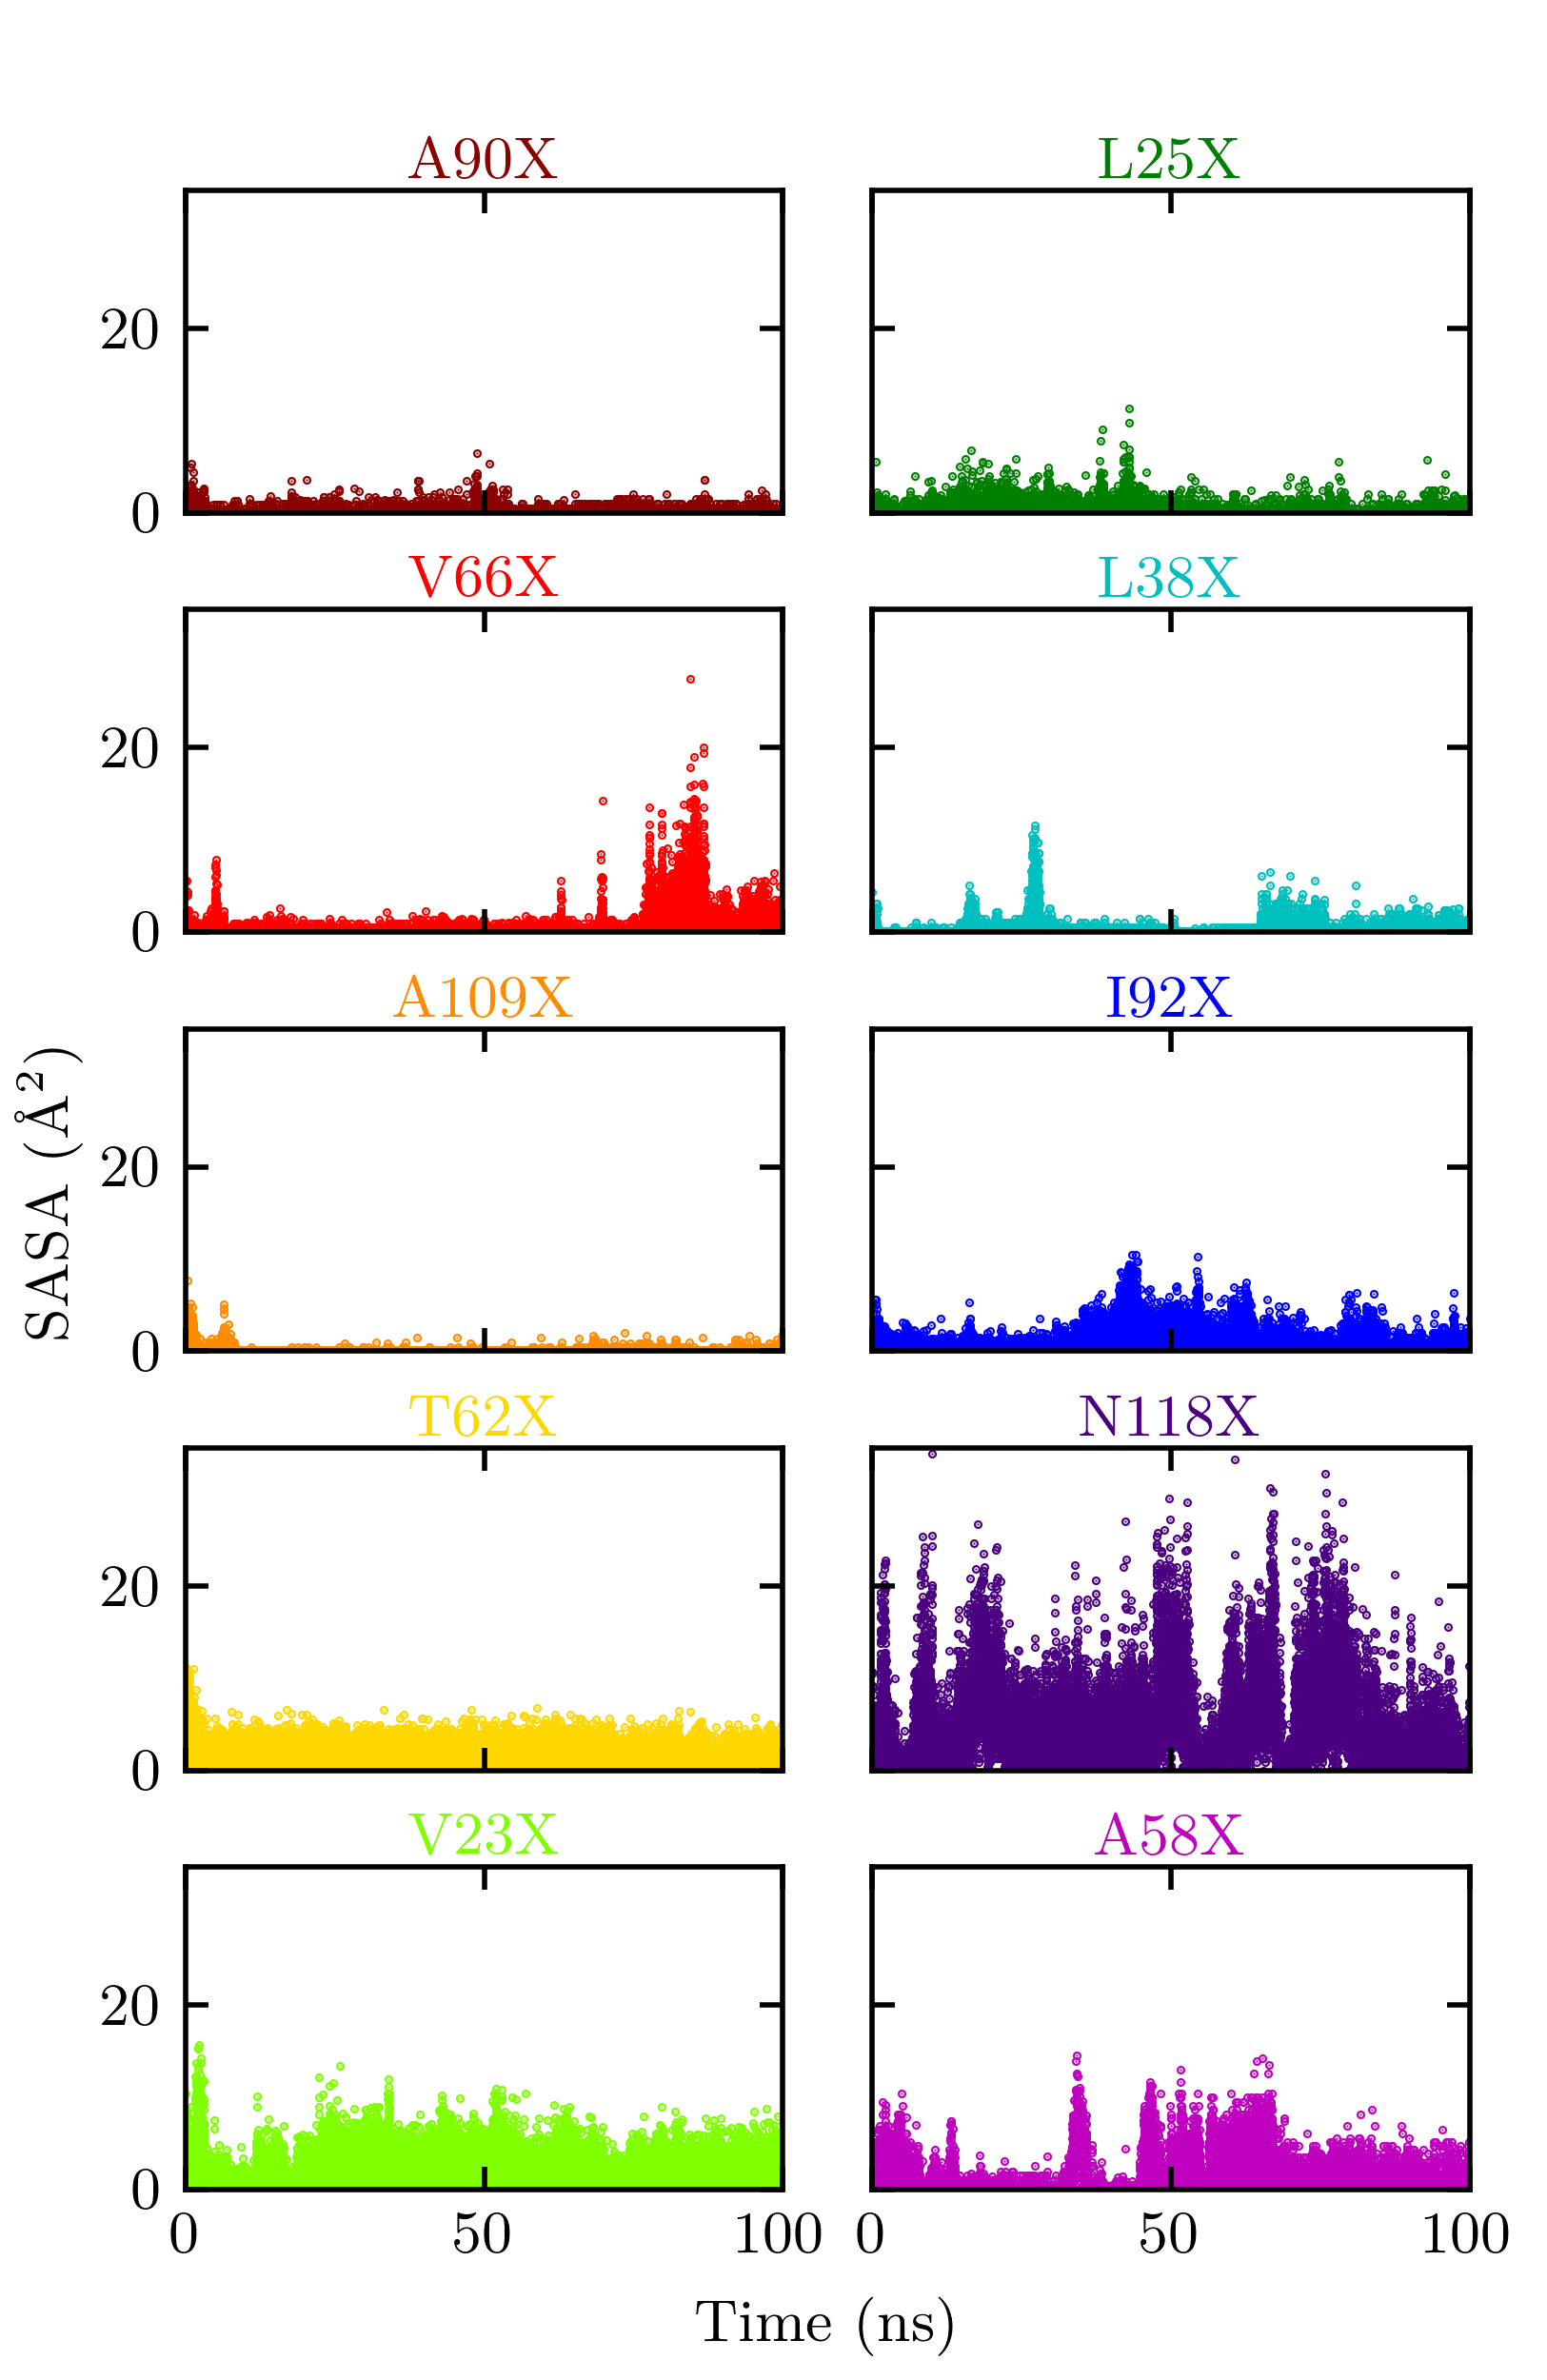
\includegraphics[width=\single]{figures-snase/sasa_sidechain_v_time.png}
    \caption[SASA of the CNC residue in each SNase location]{
        SASA of the CNC residue as a function of simulation time in 100 ns of production MD simulation for the ten SNase mutants containing the nitrile group.
    }
    \label{fig:snase-sasa}
\end{figure}

\begin{figure}
    \center
    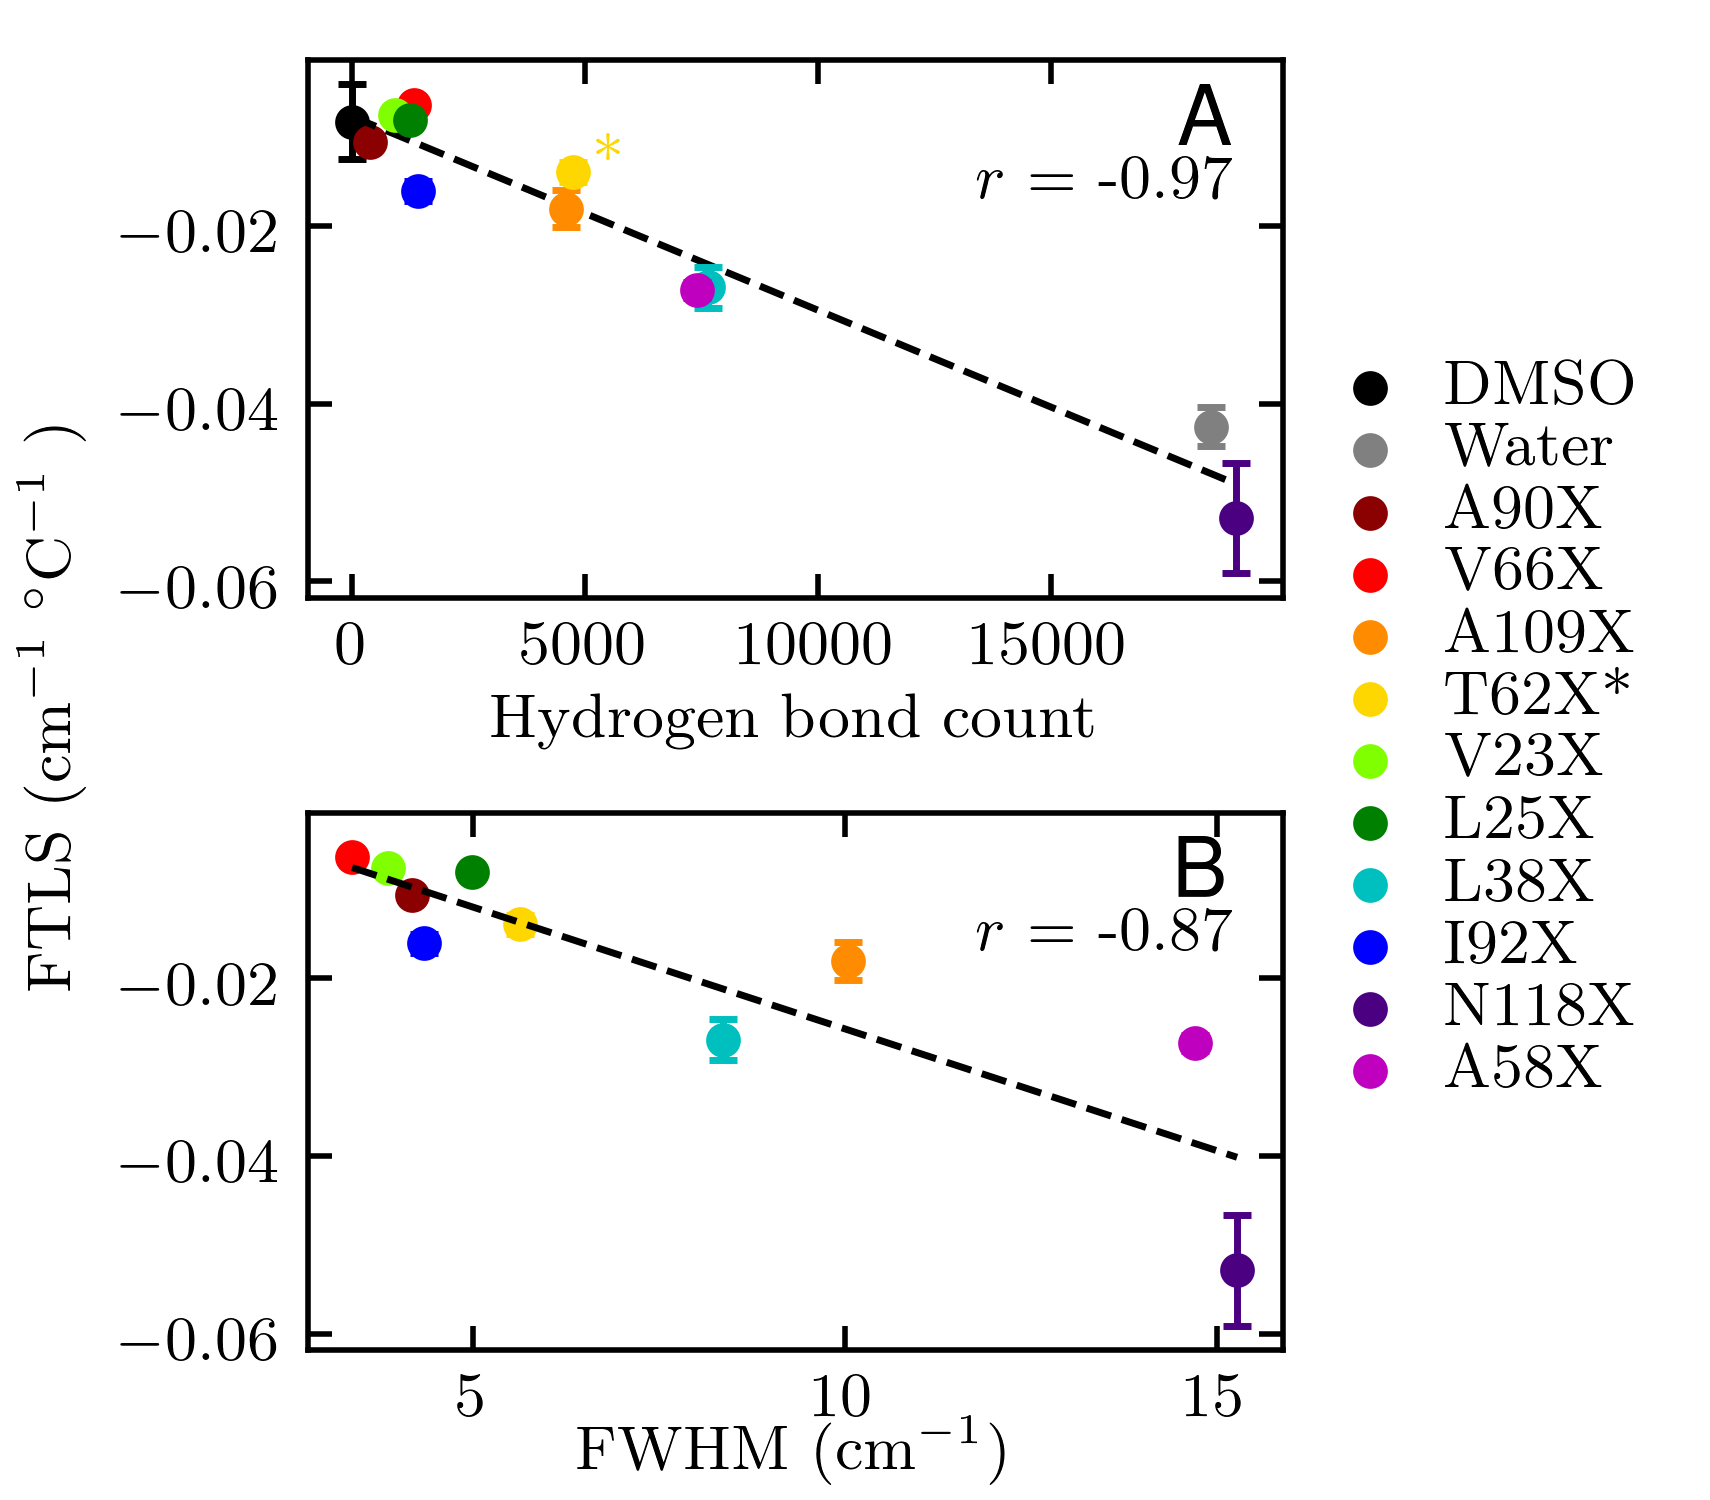
\includegraphics[width=\single]{figures-snase/combined_ftls_figures.png}
    \caption[FTLS is an experimental measurement of hydrogen bonding]{
        The frequency temperature line slope (FTLS) is an experimental measurement of hydrogen bonding. 
        (A)The measured FTLS compared to the total number of hydrogen bonding observations from simulation. 
        MeSCN in DMSO (black) was set at zero because it is aprotic. 
        MeSCN in water (gray) was extrapolated from a 20 ns MD simulation of an acetyl-CNC-NH2 peptide in water. 
        The asterisk indicates that the hydrogen bonds donated from water for T62 were not included for this comparison, as discussed in the main text. 
        (B) The measured FTLS compared to the experimental FWHM. 
        MeSCN measured in water and DMSO are excluded because we do not expect a small molecule nitrile in solution to broaden similarly to a nitrile moiety in a protein environment. 
    }
    \label{fig:snase-ftls_vs_others}
\end{figure}

This result is consistent with our previous result in GFP, where the calculated SASA of the larger \emph{p}-cyanophenylalanine probe was well correlated to the measured FTLS \cite{First2018}. 
Because the FTLS of two different types of nitrile probes are quantitively related to measurements of hydrogen bonding environment in two structurally different protein systems, this suggests that the FTLS can generally be used to quantitatively measure the hydrogen bonding status of a nitrile probe \emph{in situ}, even in the absence of the MD simulations done here. 
Therefore, the FTIR vibrational frequencies, the FWHM of the nitrile spectra, and the FTLS results offer three orthogonal, experimental, steady-state measurements to assess the local environment of the nitriles that can be compared and contrasted. 
Indeed, when plotted against each other, the FTLS and FWHM are well-correlated (Figure \ref{fig:snase-ftls_vs_others}B, $r = -0.87$) demonstrating that these two measurements are both responding to similar influences from chemical heterogeneity. 
FWHM of vibrational spectra have been previously used to assess local environment in terms of polarity with a different molecular probe \cite{Manor2012}. 
Our results suggest that, using routine FTIR instrumentation, the FTLS and FWHM of nitrile spectra generally report on specific local interactions beyond macroscopic polarity.

The apparent lack of correlation between the \dpKa{} values reported by Garcia-Moreno and coworkers and the nitrile frequencies in the same positions measured in this work (Figure \ref{fig:snase-pKas_vs_peak}), suggests that these two types of probes did not respond equally to the same interactions. 
Given that the lysine and glutamate \pKa{} shifts were also not correlated to each other for several of the locations studied here (Figure \ref{fig:snase-pKas_vs_peak}C), local interactions appear to play a significant and varied role in how the response of all three probes should be interpreted in each experiment. 
We can now revisit Figure \ref{fig:snase-pKas_vs_peak} in light of the specific observations of hydrogen bonding from our MD simulations. 
In particular, the two different \pKa{} probes were only in good agreement for locations in which a nitrile experienced bulk-like solvent hydrogen bonding (N118X) or very little hydrogen bonding (A90X, V66X, V23X, L25X, and I92X) in simulations. 
In these environments, it is likely that the glutamate and lysine \pKa{} probes interacted similarly with their surroundings. 
The two different \pKa{} probes were in poor agreement for locations that had significant hydrogen bonding, but not to bulk-like solvent (A109X, T62X, L38X, and A58X). 
In these locations, it is likely that glutamate and lysine are interacting differently with their surroundings. 
While \dpKa{} measurements give only a single scalar value, the nitrile spectra also contain information from the vibrational line shape, beyond that of a reported frequency, and this information could report on local interactions. 
Again, this is supported by the correlation between the measured FWHM of the spectra and the measured FTLS of the nitriles at each location (Figure \ref{fig:snase-ftls_vs_others}B), which measures the hydrogen bonding status of the nitrile probe. 
Coupled with MD simulations, the FWHM and FTLS measurements provide information-rich controls for understanding the contributions of hydrogen bonding to the nitrile spectra in ways that do not rely purely on the absolute absorption energy of the nitrile. 
By contrast, there is not an equivalent experimental measure of hydrogen bonding for \pKa{} probes, and it is therefore difficult to distinguish between hydrogen bonding contributions and Coulombic contributions to \dpKa{} measurements.

\subsection{Electric fields contribute vibrational line shape}

Xu et al. recently demonstrated that the distribution of Coulombic fields is a major contributor to spectral line shape and must be considered in conjunction with the effects of hydrogen bonding \cite{Xu2018}. 
We therefore calculated the electric field at the midpoint of the nitrile in each MD trajectory. 
Due to the inherent limitations of calculations based on a fixed-charge force field \cite{Slocum2017, Ritchie2013, Ricthie2014, Ensign2011}, we did not expect the simulations to be able to capture the absolute frequency shifts, but we hypothesized that the  accurate modeling of the local interactions could still yield the correct distributions of the fields that could be compared against spectral line shapes. 
In order to calculate the field distributions from the MD simulations, a dummy atom with a +1 charge was placed in the center of the nitrile bond; 
the electrostatic force on the dummy atom was calculated and projected along the nitrile bond vector. 
The partial charges on the carbon and nitrogen atoms of the nitrile group itself were neutralized and not considered because we have previously demonstrated that they result in a consistent and large field that overwhelms the contributions from the surrounding environment \cite{Stafford2010, Ritchie2013}. 
As expected, the averages of these fields were not correlated to the experimental vibrational frequencies (Figure \ref{fig:snase-external}A, $r = -0.27$). 
Even in cases where there were fewer hydrogen bonds in the simulations (A90X, V66X, V23X, L25X, I92X), where we would expect coulombic contributions to dominate the observed vibrational frequency, the calculated electric fields were still not correlated to the vibrational frequencies. 
This could be for several reasons: 
1) the model used to calculate the electric fields is insufficient to accurately reproduce the electrostatic environment of the nitrile probes; 
2) there were hydrogen bonding interactions that were not captured in the simulation that were present in the experiment; or 
3) local interactions beyond hydrogen bonding affected the vibrational frequency. 
These factors are not exclusive and could all be contributing to the poor correlation between experiment and a simple field calculation.

\begin{figure}
    \center
    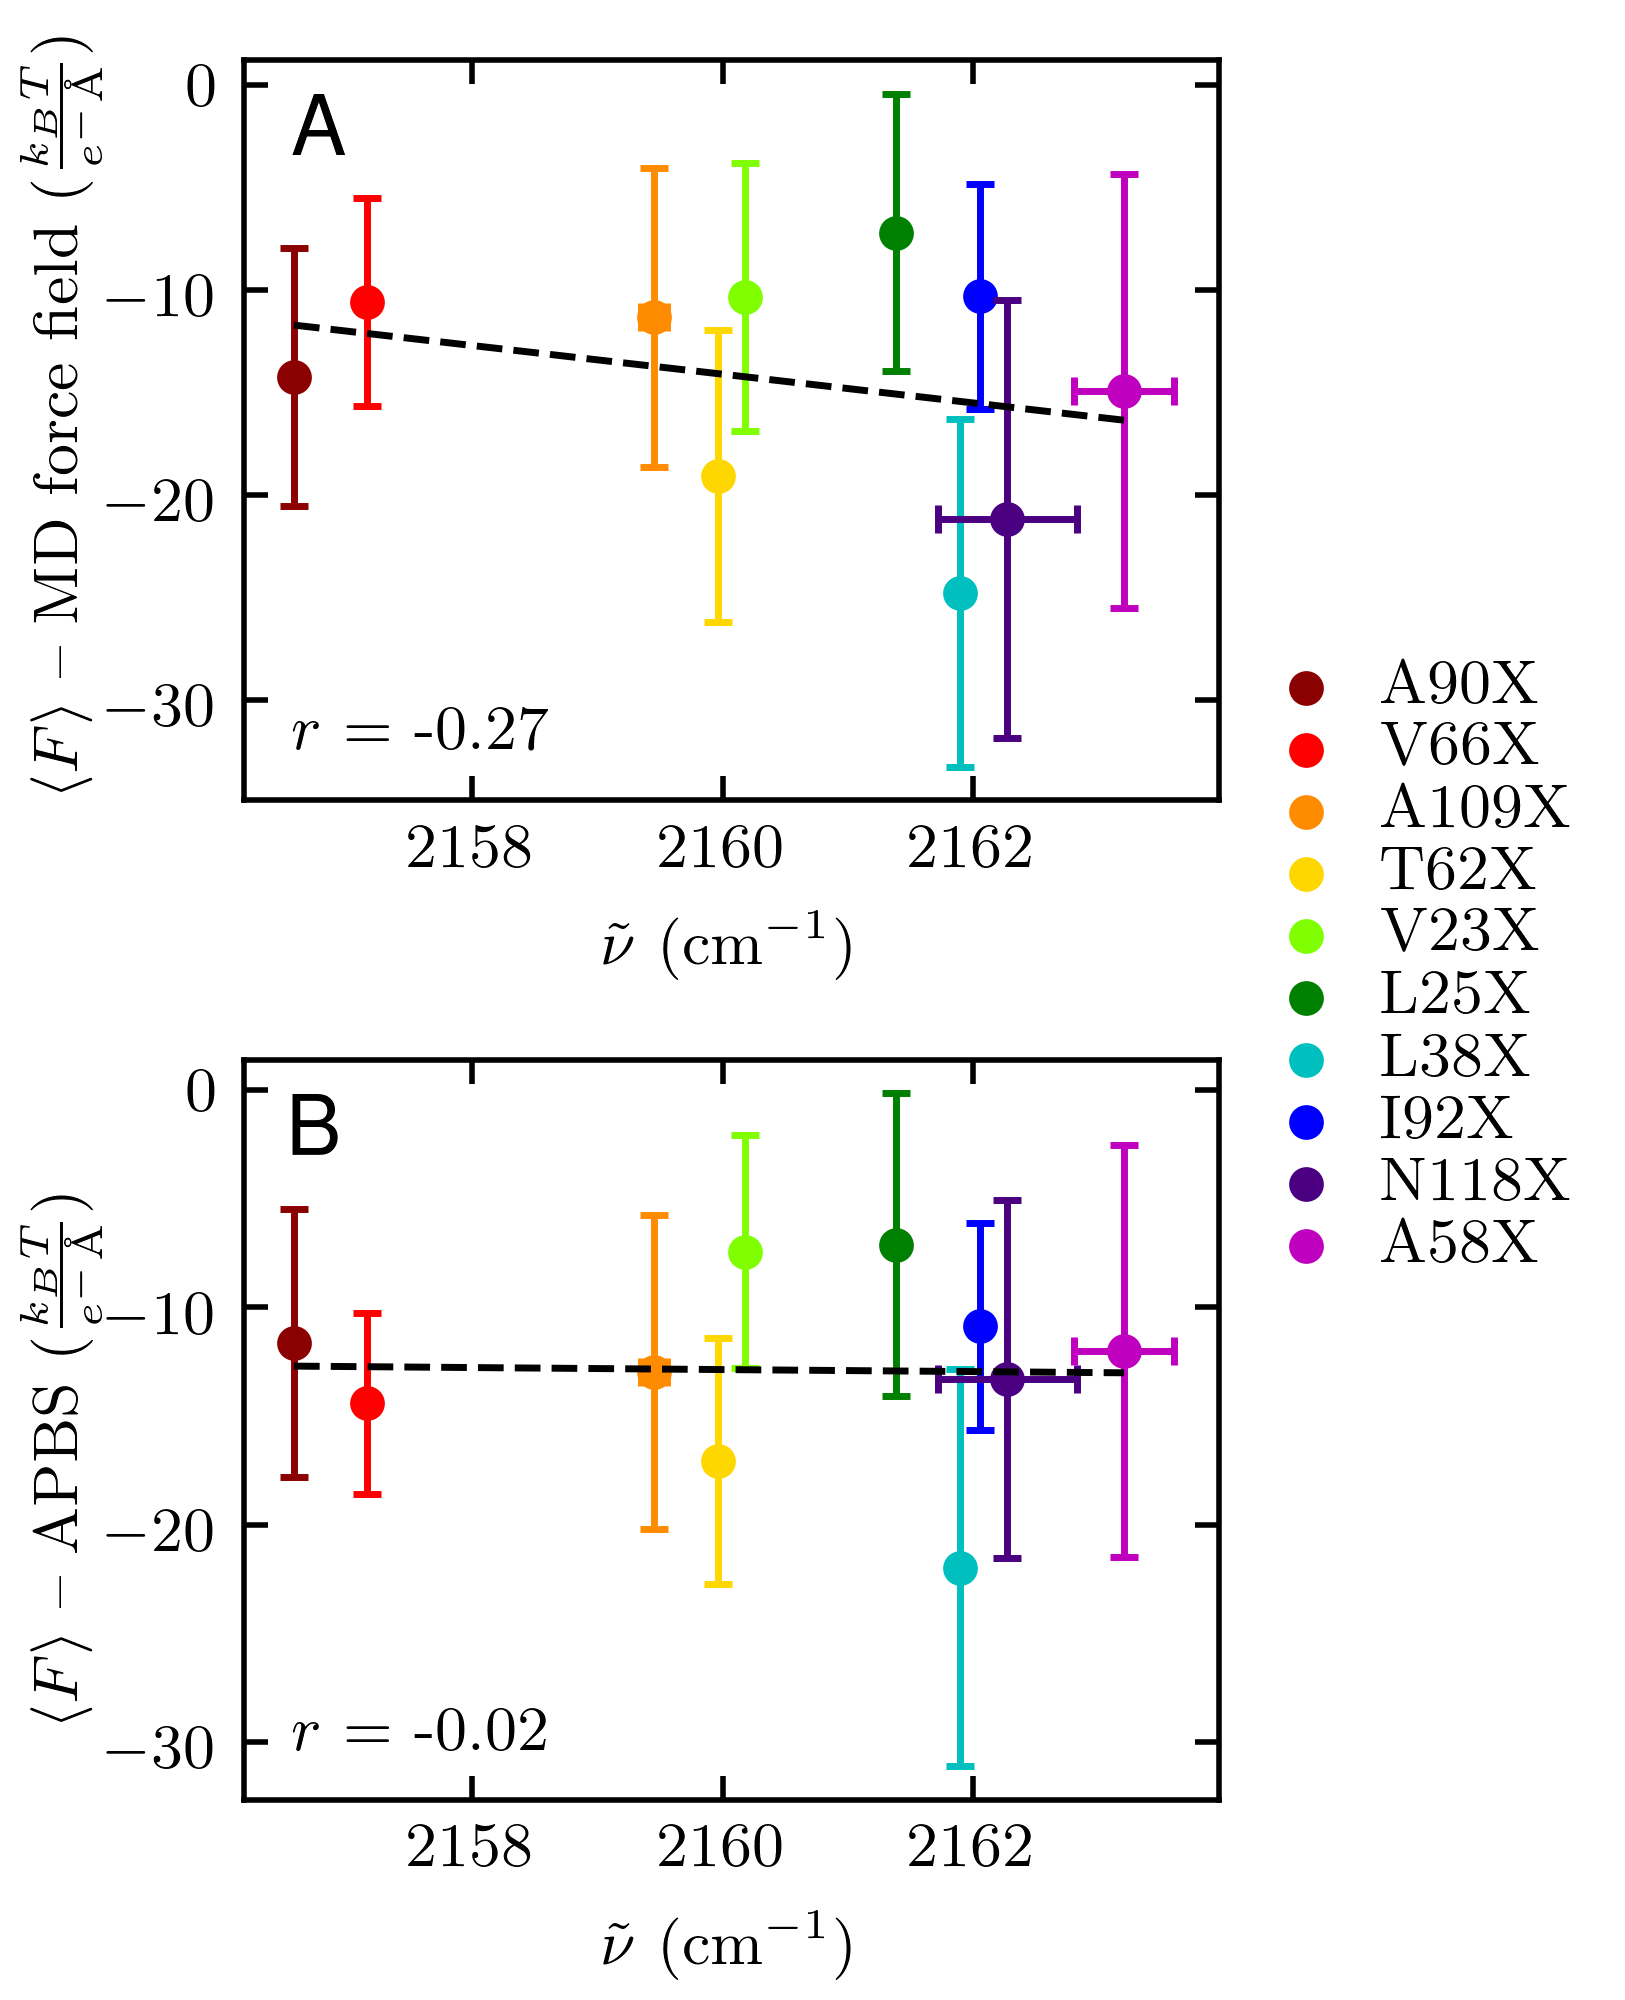
\includegraphics[width=\single]{figures-snase/combined_external_fields_figure.png}
    \caption[Calculated external fields against the observed vibrational frequencies]{
        Comparison of the calculated external fields using two different methods against the observed average peak vibrational frequencies. 
        (A) Average external field calculated using a dummy charge and the MD force field; 
        (B) Average external field calculated using the RFM method and APBS. 
        $y$-axis error bars describe the standard deviation of the distribution of the calculated field. 
        $x$-axis error bars describe the standard deviation of the peak vibrational frequency from at least three experiments.
    }
    \label{fig:snase-external}
\end{figure}

It has been suggested that continuum electrostatics models, such as the PB equation, may better capture electrostatic contributions from solvent than the direct calculation from the point-charge force field used for MD \cite{Wagoner2004}. 
In previous work, we have developed a strategy using the adaptive Poisson-Boltzmann solver (APBS) for nitrile-containing proteins, referred to as the reaction field method (RFM), that calculates the external field from two components: 
the solvent reaction field (SRF), which only includes contributions from the solvent atoms, and 
the protein Coulomb field (PCF), which only includes contributions from the protein atoms. 
This strategy has been shown to mitigate the error intrinsic in the numerical integration of the PB equation for the calculation of the SRF \cite{Ritchie2013, Ritchie2014, Ritchie2015}. 
We therefore also calculated the external field at the midpoint of the nitrile using the RFM with APBS for each of our nitrile containing SNase constructs. 
Because the SRF calculated with APBS at each time point required two separate solutions to the PB equation (which is computationally intensive), we only calculated the SRF with APBS every 100 ps of the 100 ns trajectory. 
For comparison, the fields calculated directly from the MD force field were evaluated every 4 ps. 
In spite of the more complex APBS calculations, the RFM calculated external fields were not correlated to the experimental frequencies (Figure \ref{fig:snase-external}B, $r = -0.02$). 
To investigate this further, we compared the individual components of the RFM (the SRF and the PCF) to the corresponding components calculated directly from the MD force field. 
The SRF calculated with APBS as a function of time is shown in Figure \ref{fig:snase-apbs}A, and the SRF calculated directly from the MD force field as a function of time is shown in Figure \ref{fig:snase-md_field}A. 
Both the SRF calculated with APBS and the SRF calculated directly from the MD force fields captured the same changes in field over time, but the density of data for the direct MD calculation offers more information because the less expensive calculation can be performed more frequently, providing increased time resolution. 
The more expensive APBS calculation produced data with lower time resolution and did not provide additional accuracy. 
The averages of the SRF calculated with APBS were strongly correlated (Figure \ref{fig:snase-apbs}B, $r = 0.81$) to the averages of the SRF calculated directly from the MD force field. 
For the PCF component, the RFM and the direct calculation from the MD force field both report the sum of the Coulombic interactions, and therefore the averages were well correlated, as expected (Figure \ref{fig:snase-apbs}C, $r = 0.94$). 
Given that the field directly calculated from the MD force field reported equivalent fields over time with increased sampling compared to fields calculated with APBS, we continued our investigation using only the fields calculated directly from the MD force field.

\begin{figure}
    \center
    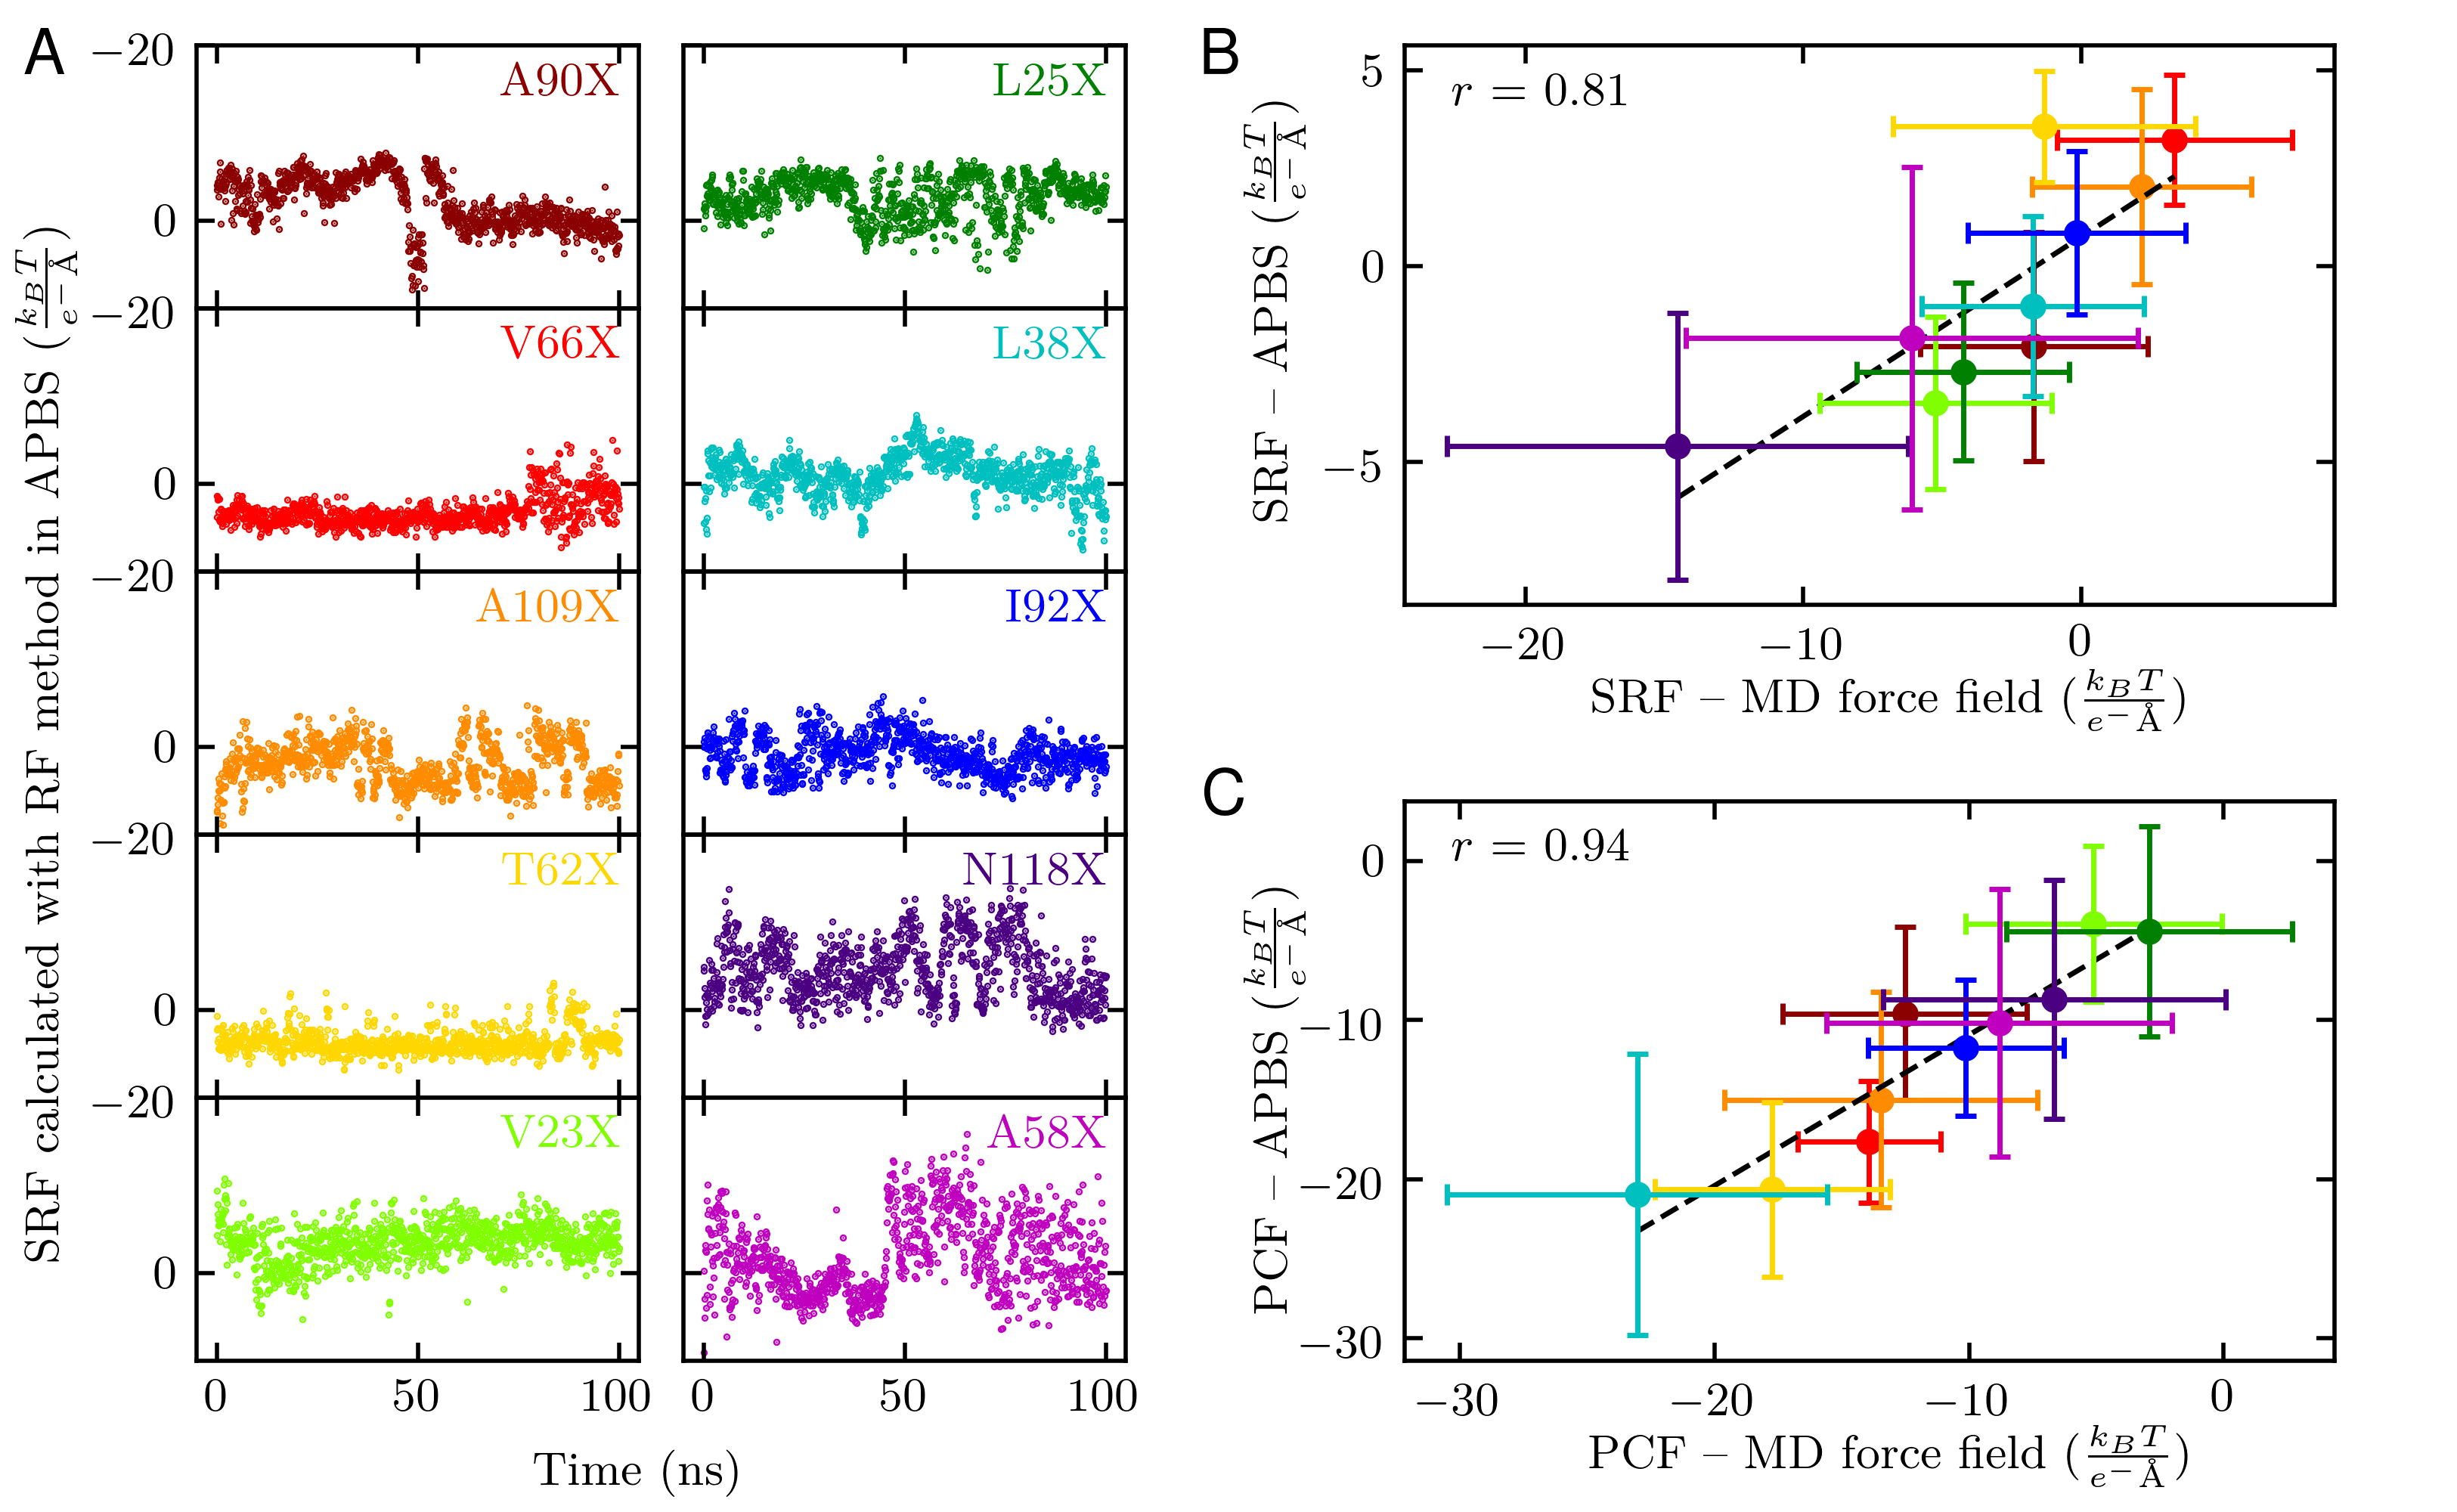
\includegraphics[width=\double]{figures-snase/combined_APBS_figure.png}
    \caption[Comparison of field calculated using APBS to the field calculated using the MD force field]{
        Comparison of field calculated using APBS to the field calculated using a dummy atom and the MD force field. 
        (A) The SRF calculated using the RFM and APBS as a function of time in each simulation. 
        (B) The average SRF calculated using the RFM and APBS against the average SRF calculated directly from the MD force field using a dummy charge. 
        (C) The average PCF calculated using the RFM and APBS against the average PCF calculated directly from the MD force field using a dummy charge. 
        (B\&C) Points are colored according to the corresponding mutant in panel A. 
        Error bars on both axes represent the standard deviation of the distribution of calculated field.
    }
    \label{fig:snase-apbs}
\end{figure}

\begin{figure}
    \center
    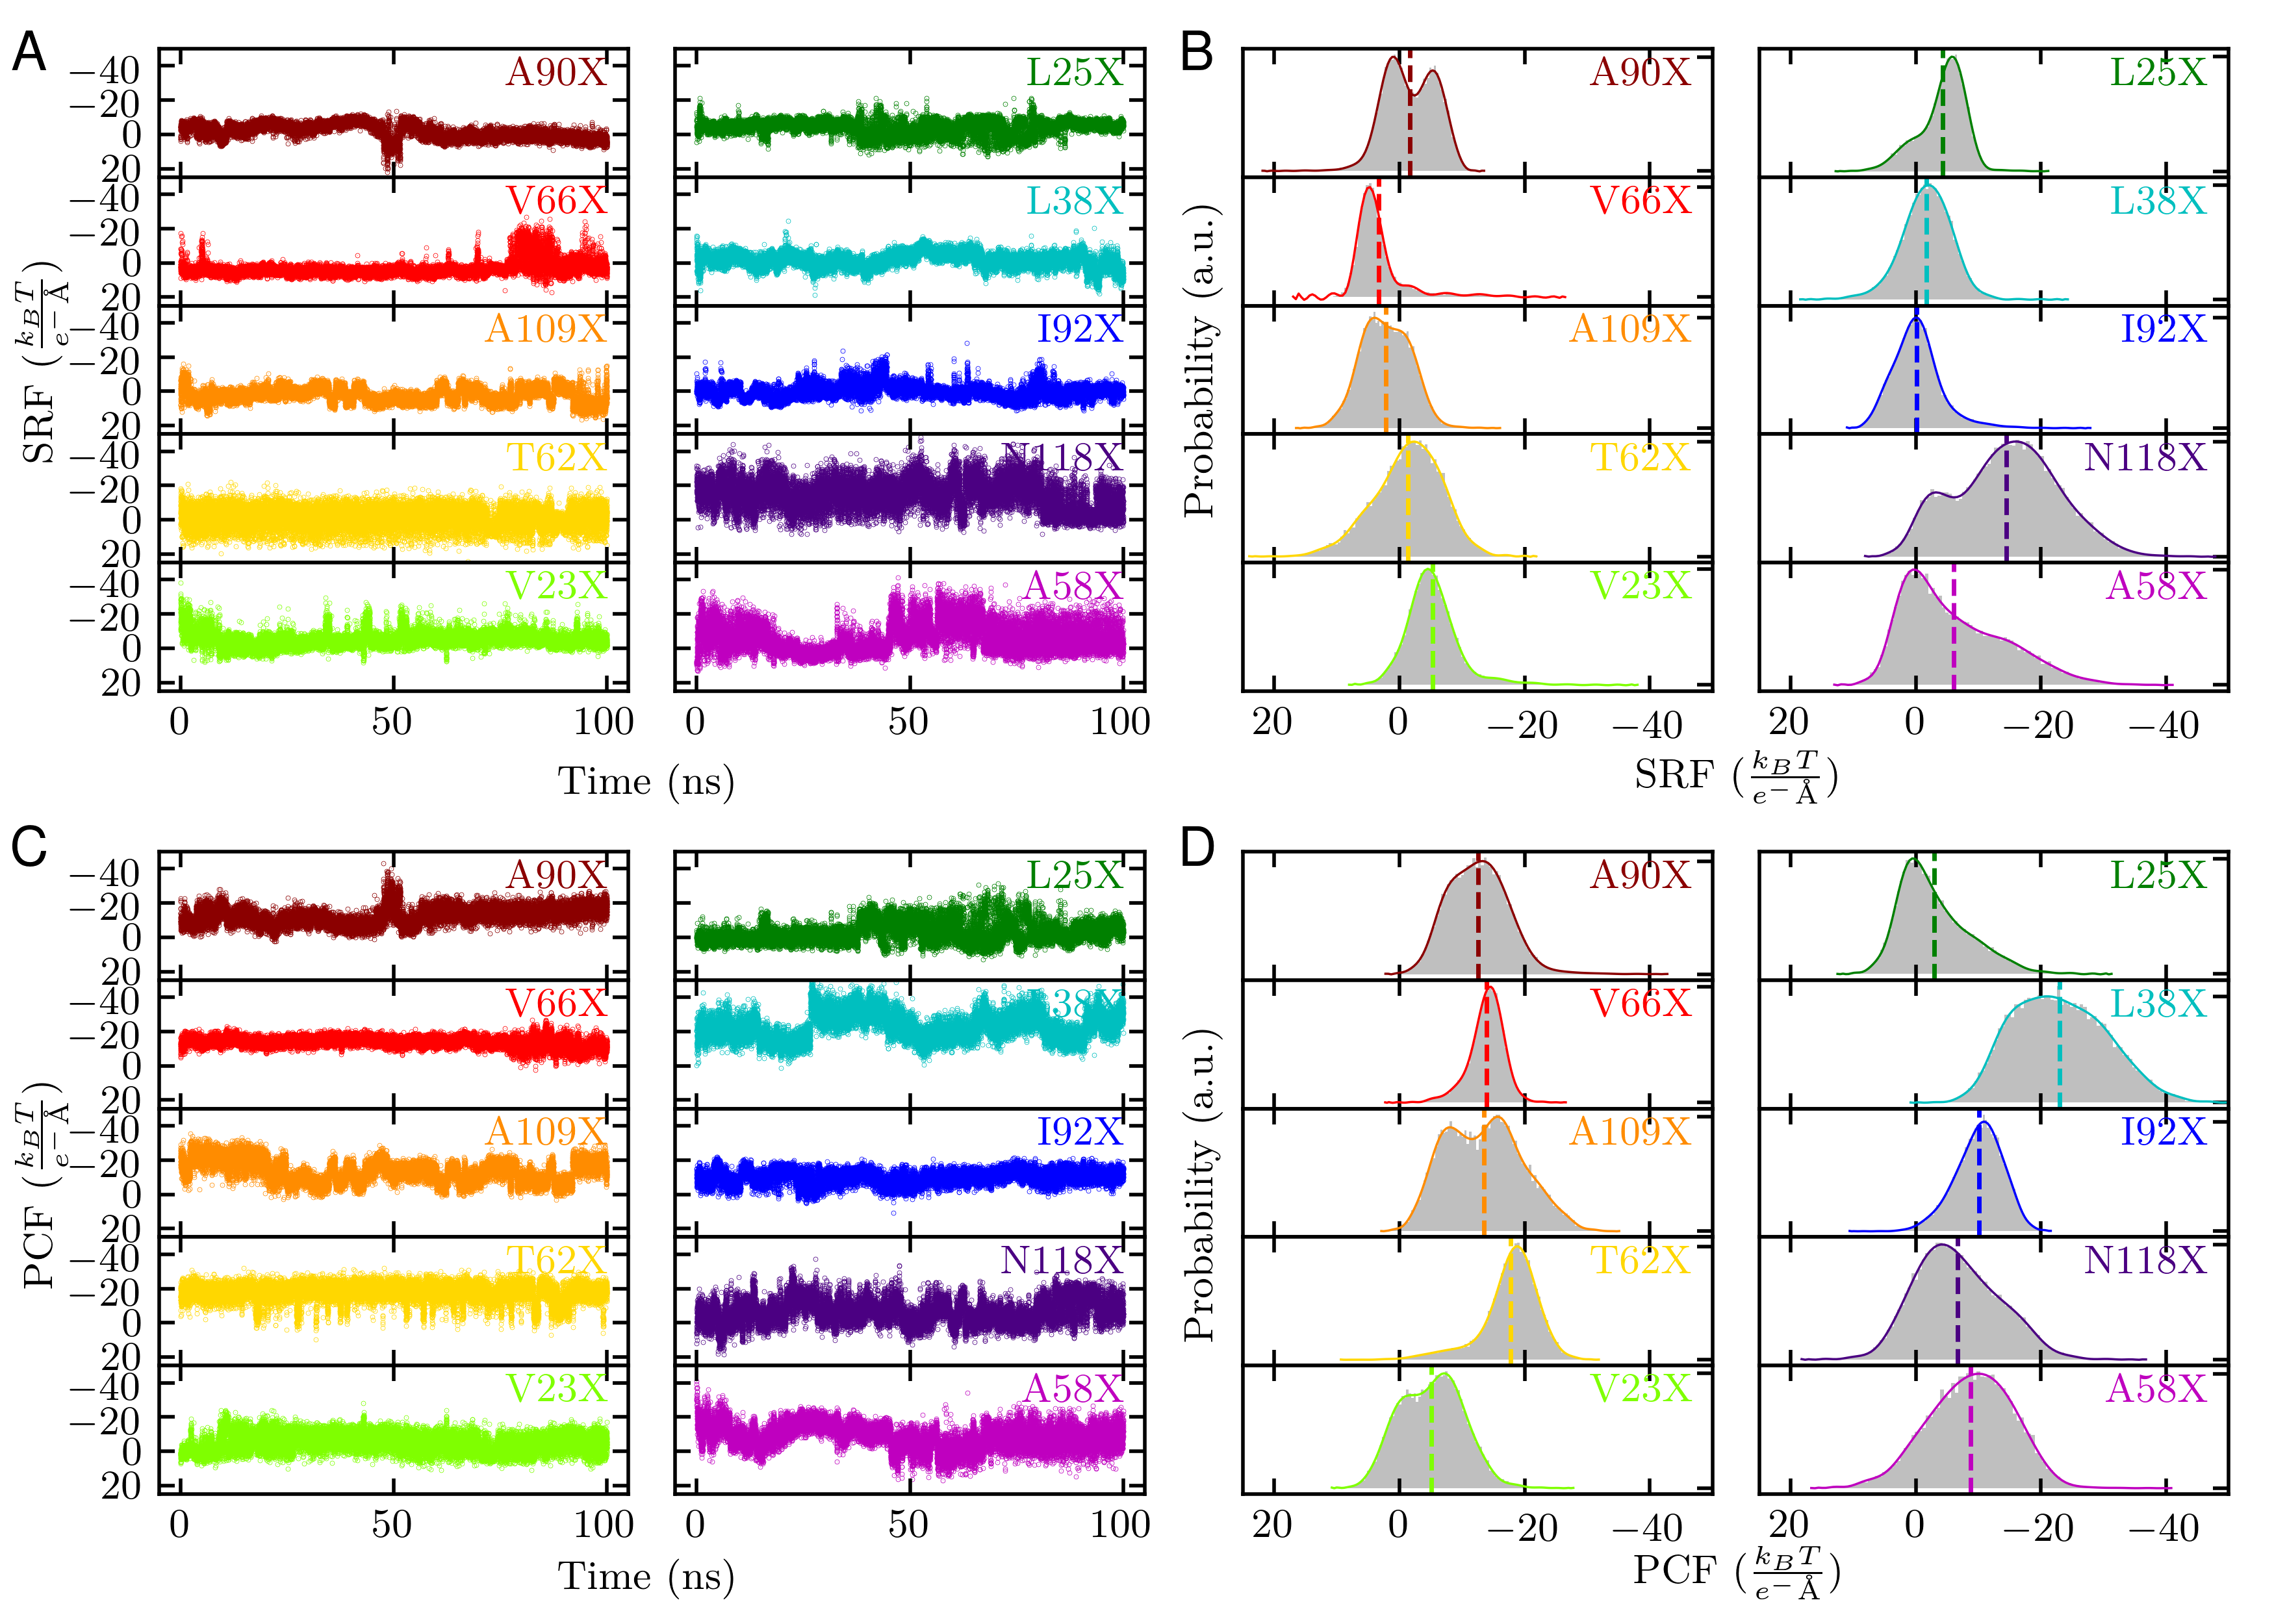
\includegraphics[width=\double]{figures-snase/combined_figure_fields.png}
    \caption[]{
        Calculated components of the electric field at the midpoint of the nitrile at each location. 
        (A) The SRF as a function of time. 
        (B) Histograms of the calculated SRF. 
        (C) The PCF as a function of time. 
        (D) Histograms of the calculated PCF. 
        (B\&D) Gray: probability of the nitrile experiencing a particular field; 
        solid colored lines: polynomial fit to the histograms; 
        vertical dashed lines: mean field experienced by the nitrile. 
        Note that the $y$-axes in A\&C and $x$-axes in B\&D are reversed to reflect the negative difference dipole moment of the CNC nitrile moiety.
    }
    \label{fig:snase-md_field}
\end{figure}

To investigate the \emph{distribution} of the fields experienced by the nitrile in each system, we binned the calculated SRF and PCF for each nitrile, and we fit a polynomial to the histograms of each component (Figures \ref{fig:snase-md_field}B,D, respectively). 
Of the probes that exhibited narrow FTIR spectra, A90X, V66X, V23X, L25X, and I92X, most had similarly narrow distributions of SRF and PCF.  
A90X and L25X, however, exhibited field distributions that were more complicated than expected based on their FTIR spectra. 
From the calculations of SRF and PCF over the length of the trajectory (Figure \ref{fig:snase-md_field}A,C), we observed distinct changes in these fields. 
To determine the cause of these changes, we calculated the $\chi_1$ and $\chi_2$ dihedral angles of the CNC probe (illustrated in Figure \ref{fig:snase-hbond_criteria}) for the length of the simulations; 
these results are shown in Figure \ref{fig:snase-chi}A,B, respectively. 
Around 50 ns, the CNC residue on A90X briefly rotated around the $\chi_2$ dihedral angle, which dramatically shifted the projection of the field, causing a decrease in the SRF that was compensated by an increase in the PCF. 
These two populations resulted in a double-peak shape for both the SRF and PCF histograms for A90X. 
Because the changes in the SRF and PCF offset each other, we concluded that these distributions were nonetheless consistent with the narrow spectrum. 
The nitrile at L25X experienced more heterogeneity in both dihedral angles, resulting in a greater variety of sampled conformations for the nitrile probe. 
All of those conformations, however, had similar PCF and SRF projections, resulting in a broader distribution of fields, and the FTIR spectrum for L25X was broader than the others.

\begin{figure}
    \center
    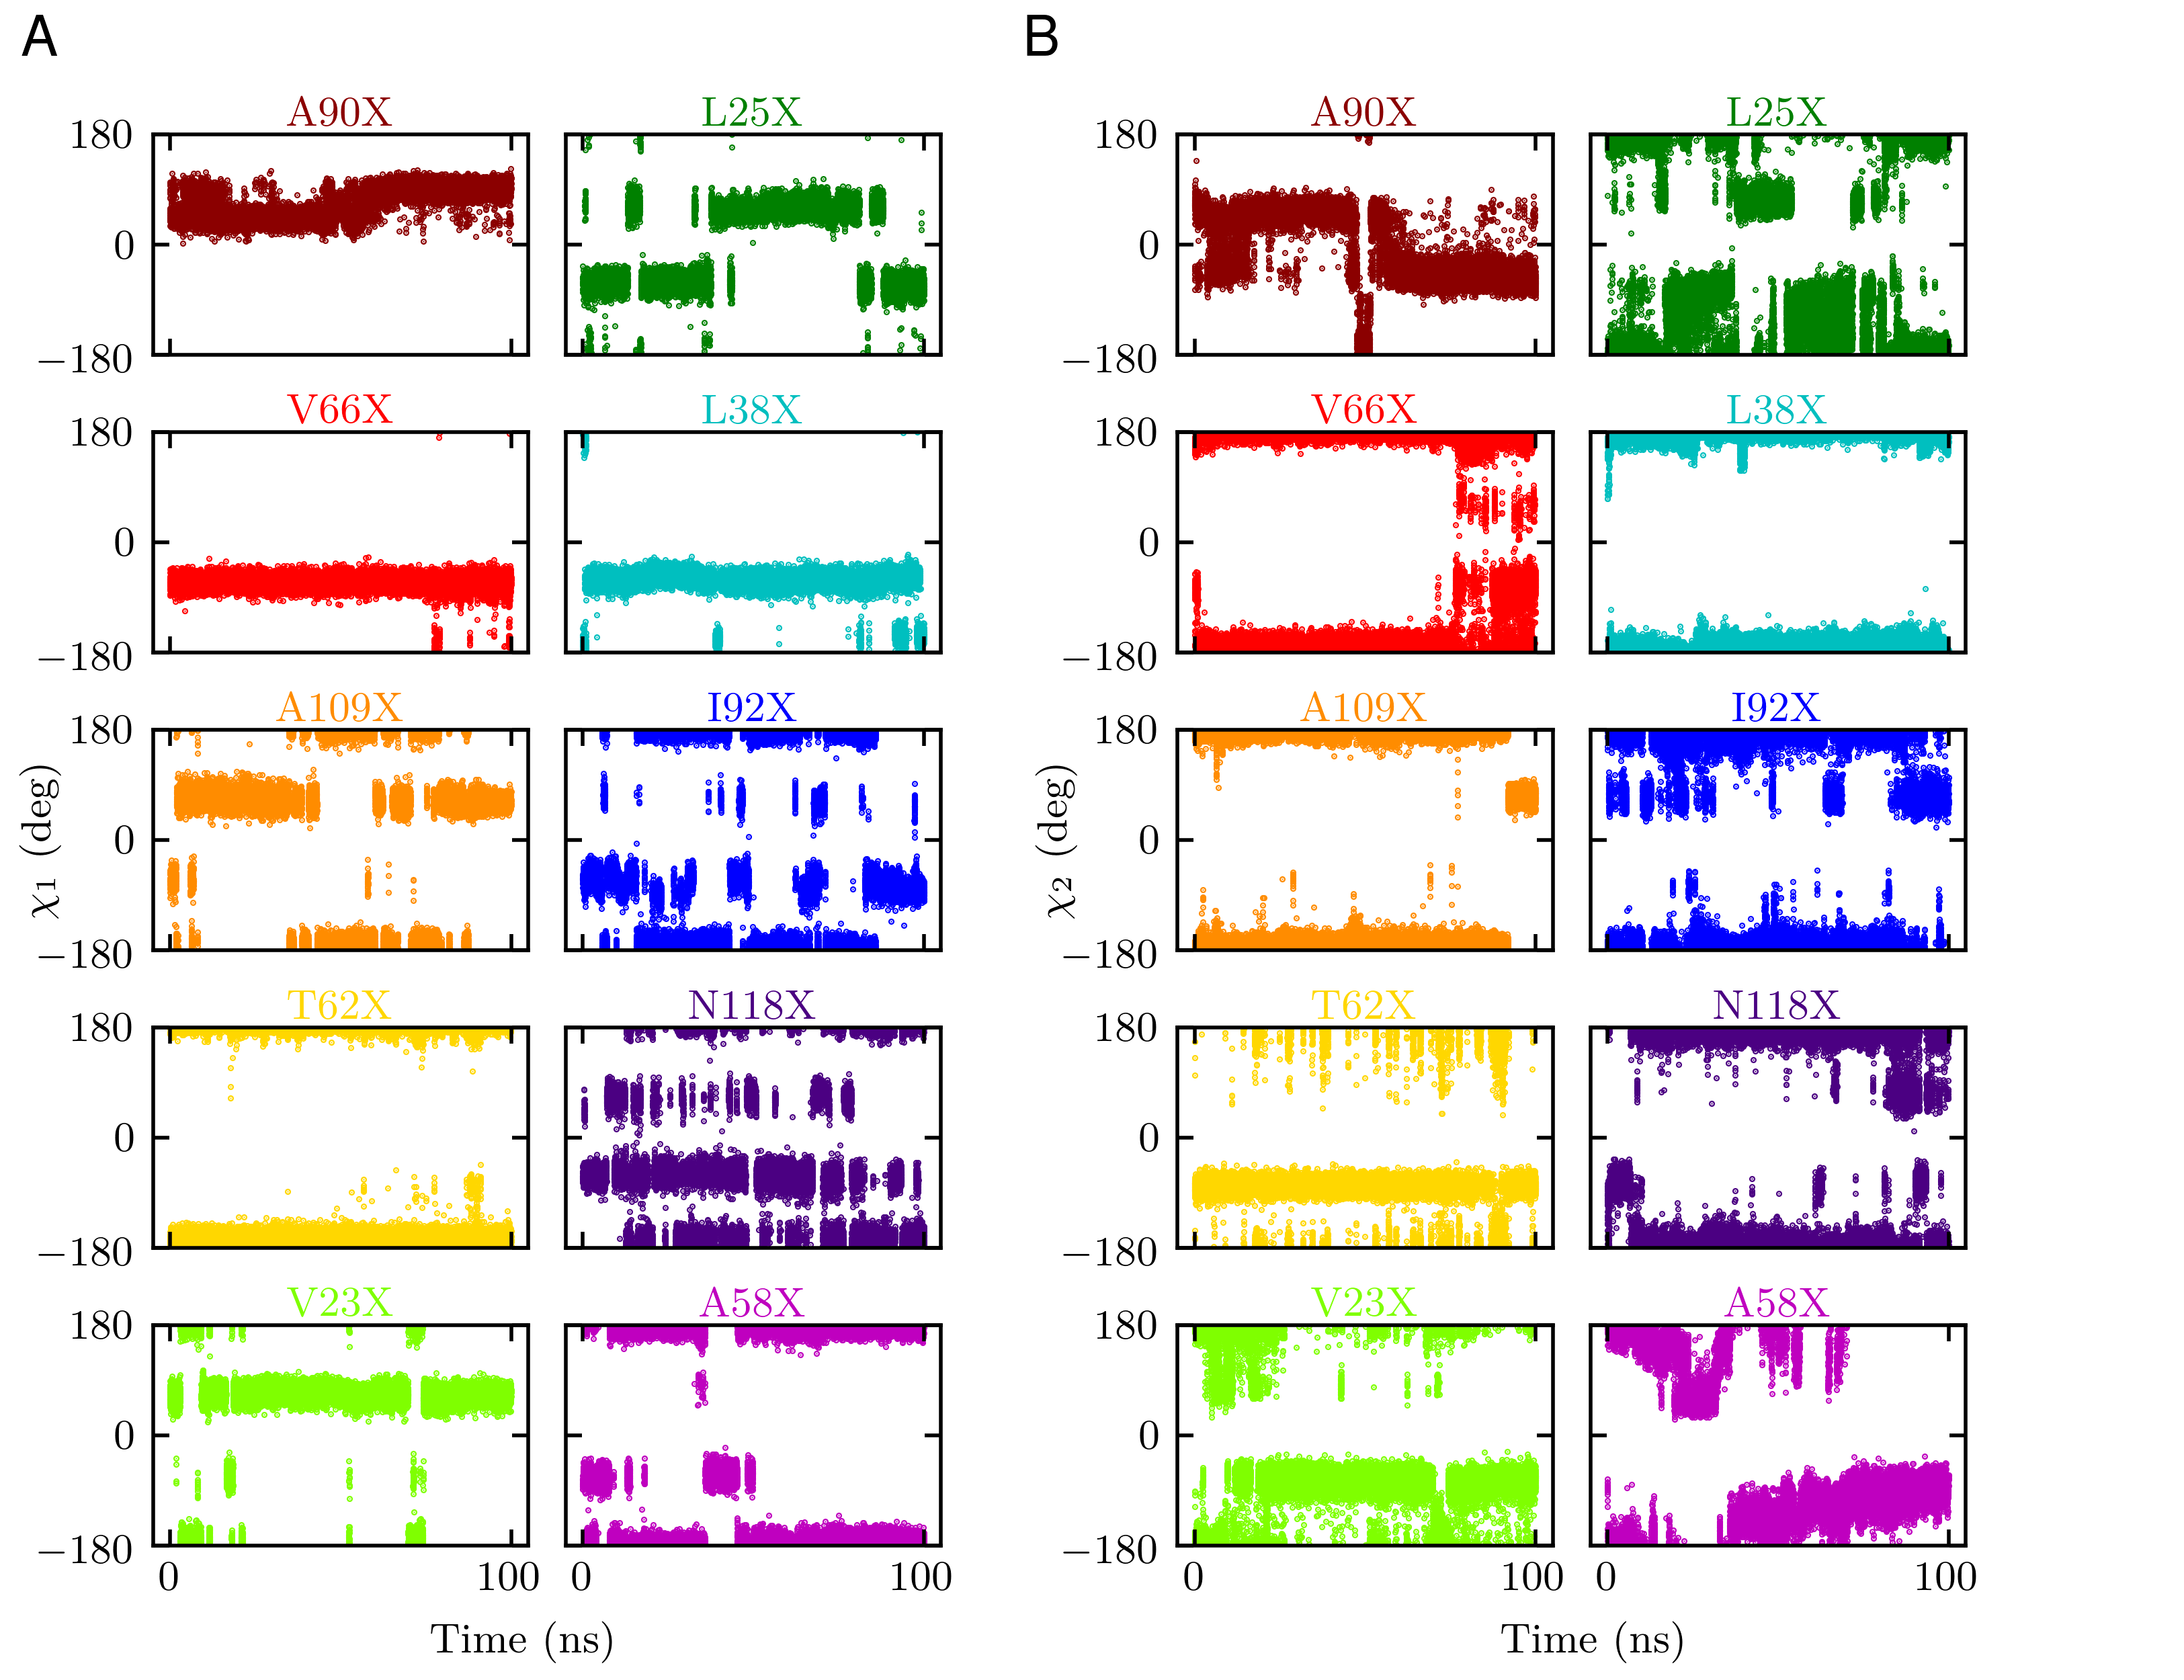
\includegraphics[width=\double]{figures-snase/combined_chi.png}
    \caption[Dihedral angle sampling of the CNC probe at each location]{
        Dihedral angle sampling of the CNC probe at each location. 
        (A) The $\chi_1$ dihedral angle determined for each construct as a function of simulation time. 
        (B) The $\chi_2$ dihedral angle determined for each construct as a function of simulation time. 
        These two dihedral angles are illustrated in Figure \ref{fig:snase-hbond_criteria}.
    }
    \label{fig:snase-chi}
\end{figure}

The nitriles at A109X, T62X, and L38X experienced more heterogeneity of the SRF and PCF over the course of the trajectory. 
For A109X, rotations about $\chi_1$ and $\chi_2$ created several different states, each with a different field projection on the nitrile bond vector, resulting in a distribution of field with multiple populations. 
Accordingly, the spectrum of the nitrile at A109X was broad. 
The nitrile at T62X primarily existed in one conformation dominated by a single hydrogen-bonding interaction. 
Periodically, the probe rotated about $\chi_2$, sampling a configuration with a shifted SRF, resulting in narrow distribution of field with a separate smaller population. 
This was consistent with the observed narrow spectrum with a small shoulder. 
L38X sampled a single dihedral conformation throughout the simulation. 
However, the probe was oriented towards a flexible region of the protein (residues 114-120), and the flexibility of this loop observed in the MD simulation caused large fluctuations in the PCF, resulting in a broader distribution of the field. 
This was consistent with the broader experimental spectra.

Finally, the nitriles at N118X and A58X both experienced broadly distributed SRF and PCF. 
N118X was solvent exposed and interacted with bulk-like water, which resulted in the broadest distribution of SRF of all the probes, consistent with the large FWHM in the experimental spectrum. 
For A58X, rotations about $\chi_1$ and $\chi_2$ dihedral angles and differences in level of solvent exposure resulted in large fluctuations in the projected field. 
Correspondingly, the observed spectrum had a large FWHM and appeared to contain several overlapping populations. 
Overall, the distributions of the calculated fields qualitatively mirrored the line shapes observed in the experimental spectra.

Because of the apparent similarities between the distributions of the calculated SRF and PCF for each protein system and the experimentally observed line shape, we calculated the standard deviation of each calculated field over the length of the simulations to describe the distribution of these fields quantitatively. 
Alone, the standard deviation of either component, the SRF or the PCF, did not account for the experimentally observed FWHM (Figure \ref{fig:snase-component_std}A,B, respectively). 
This indicated that while both the SRF and the PCF may contribute, neither exclusively determines the observed line shape of the nitrile spectra. 
To determine the overall effect of the distributions of both component fields, we combined their standard deviations according to Equation \ref{eq:snase-comb_std}:
\begin{equation}
    \sigma_\text{combined}=\sqrt{\sigma^2_\text{SRF}+\sigma^2_\text{PCF}}
    \label{eq:snase-comb_std}
\end{equation}
where $\sigma_\text{SRF}$ and $\sigma_\text{PCF}$ are the individual standard deviations of the SRF and PCF distributions, respectively. 
The combined standard deviations were strongly correlated to the experimental FWHM from the nitrile spectra (Figure \ref{fig:snase-comb_std}, $r = 0.95$), suggesting that the combined information from the distributions of the component fields determined the overall peak width.

\begin{figure}
    \center
    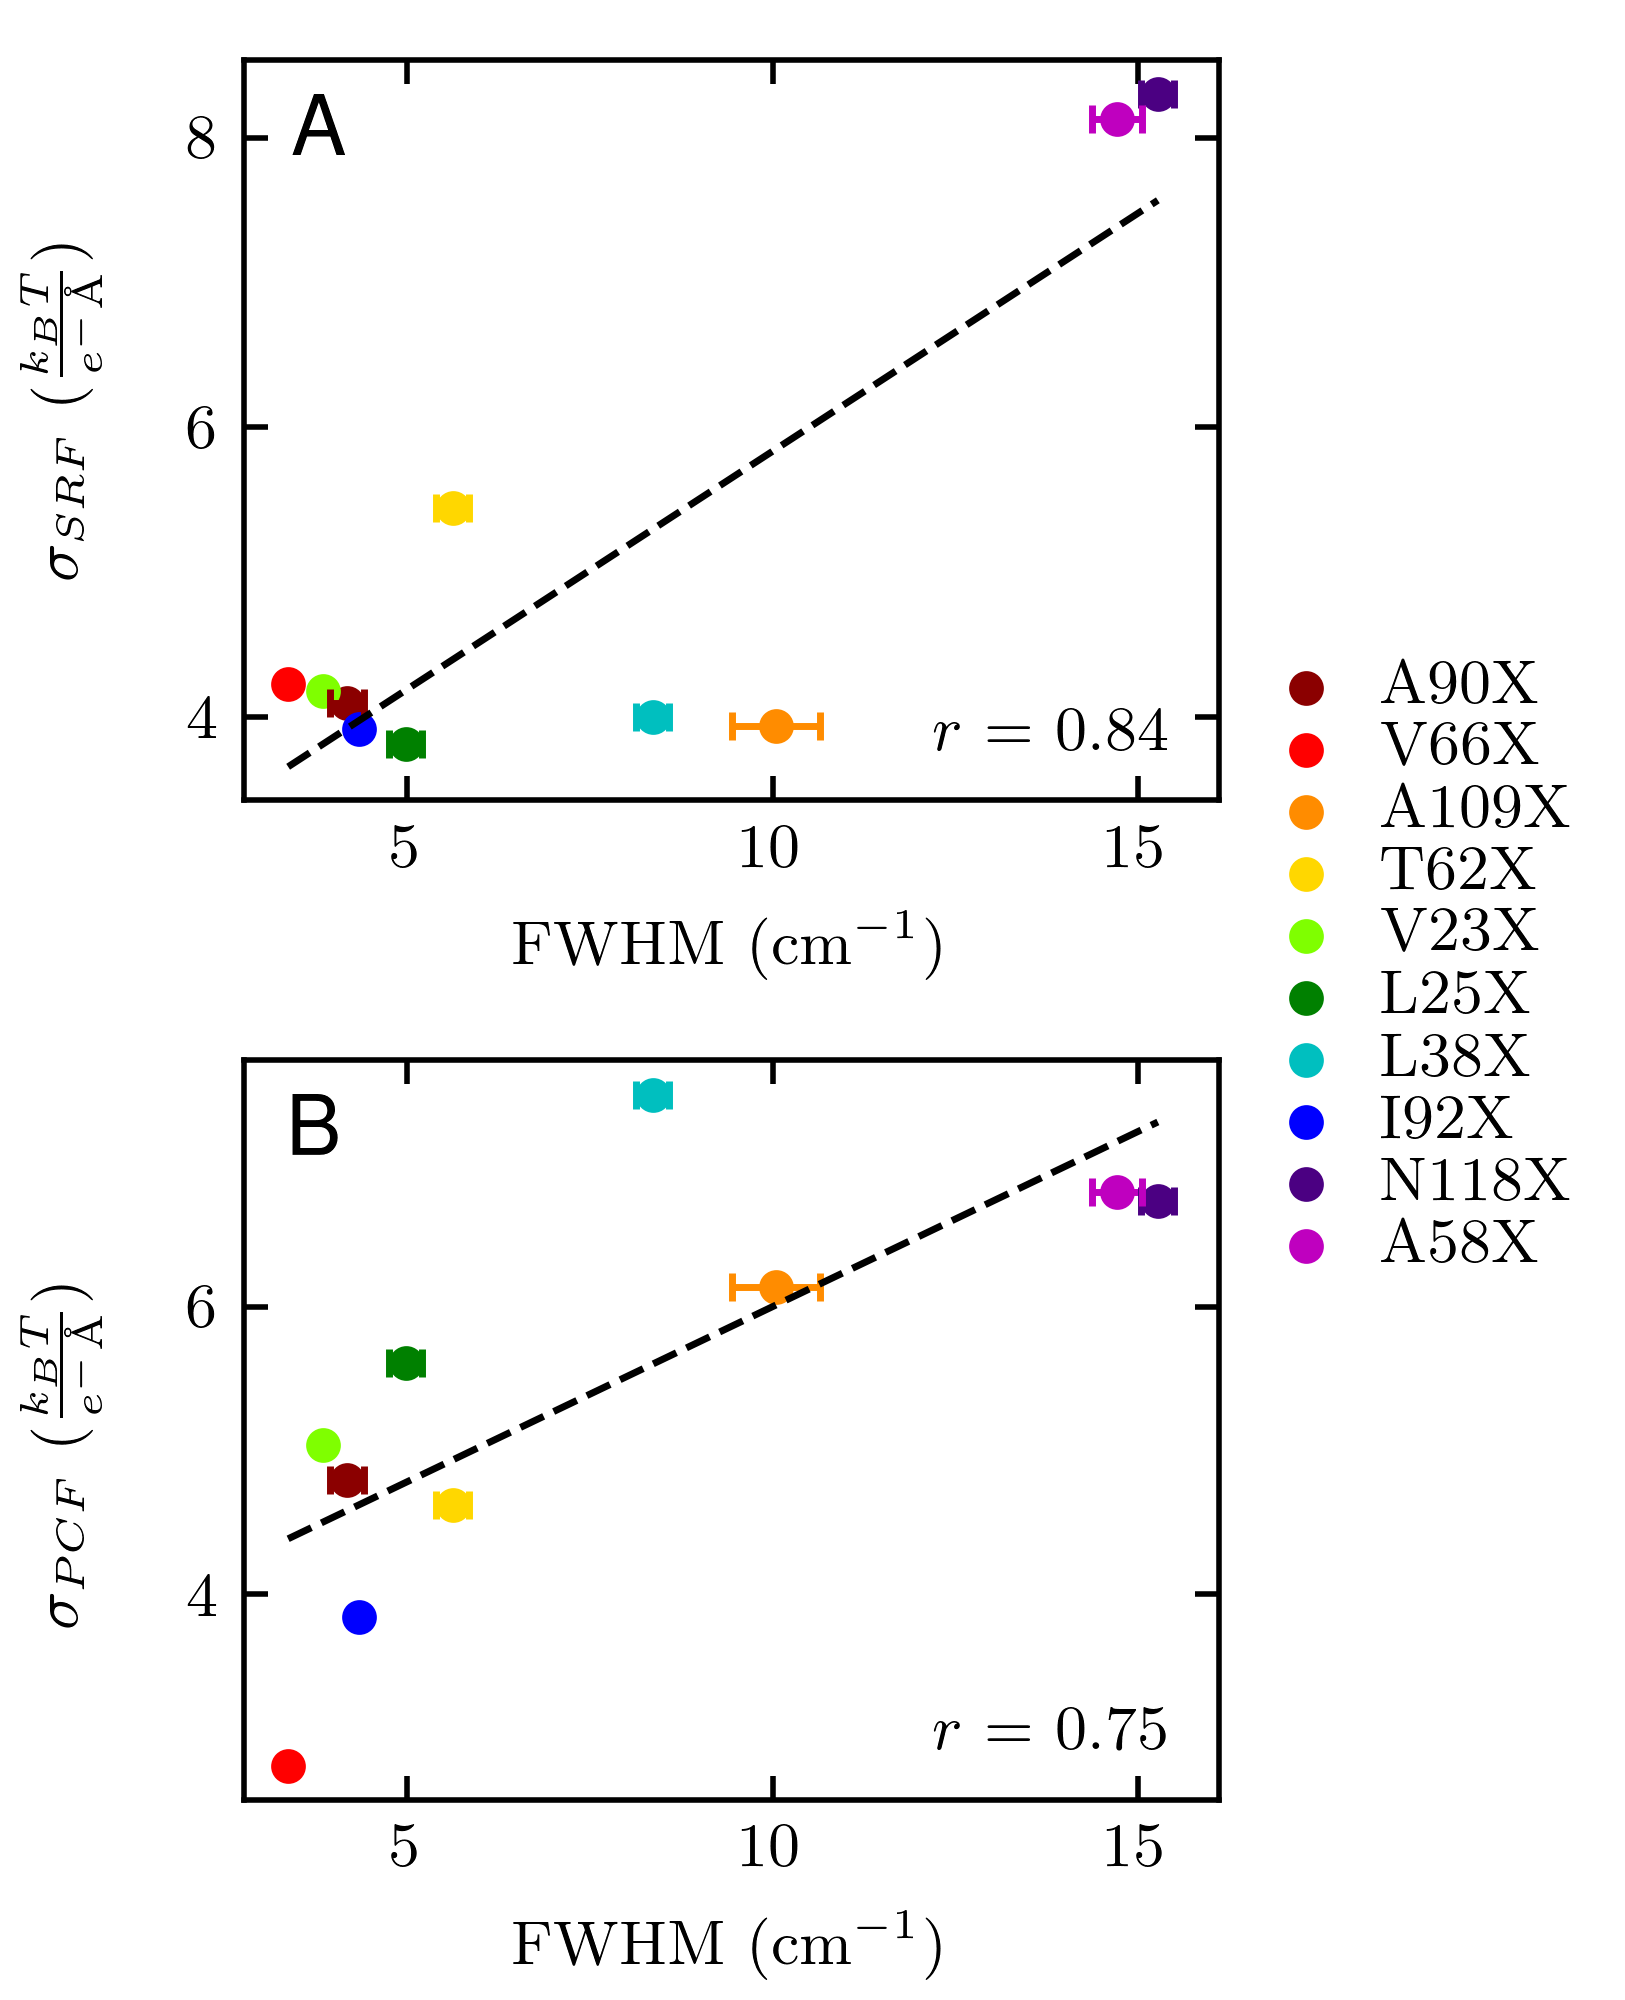
\includegraphics[width=\single]{figures-snase/combined_standard_deviations.png}
    \caption[Distribution of component fields against the experimental FWHM]{
        Comparison of the distribution of component fields against the experimental FWHM. 
        (A) The standard deviation of the SRF against the experimental FWHM of each nitrile construct. 
        Note that while the correlation constant is high, the $y$-axis is not adequately sampled. 
        (B) The standard deviation of the PCF against the experimental FWHM of each nitrile construct. 
        (A\&B) Error bars on the $x$-axes describe the standard deviation of the FWHM from at least three experiments.
    }
    \label{fig:snase-component_std}
\end{figure}

\begin{figure}
    \center
    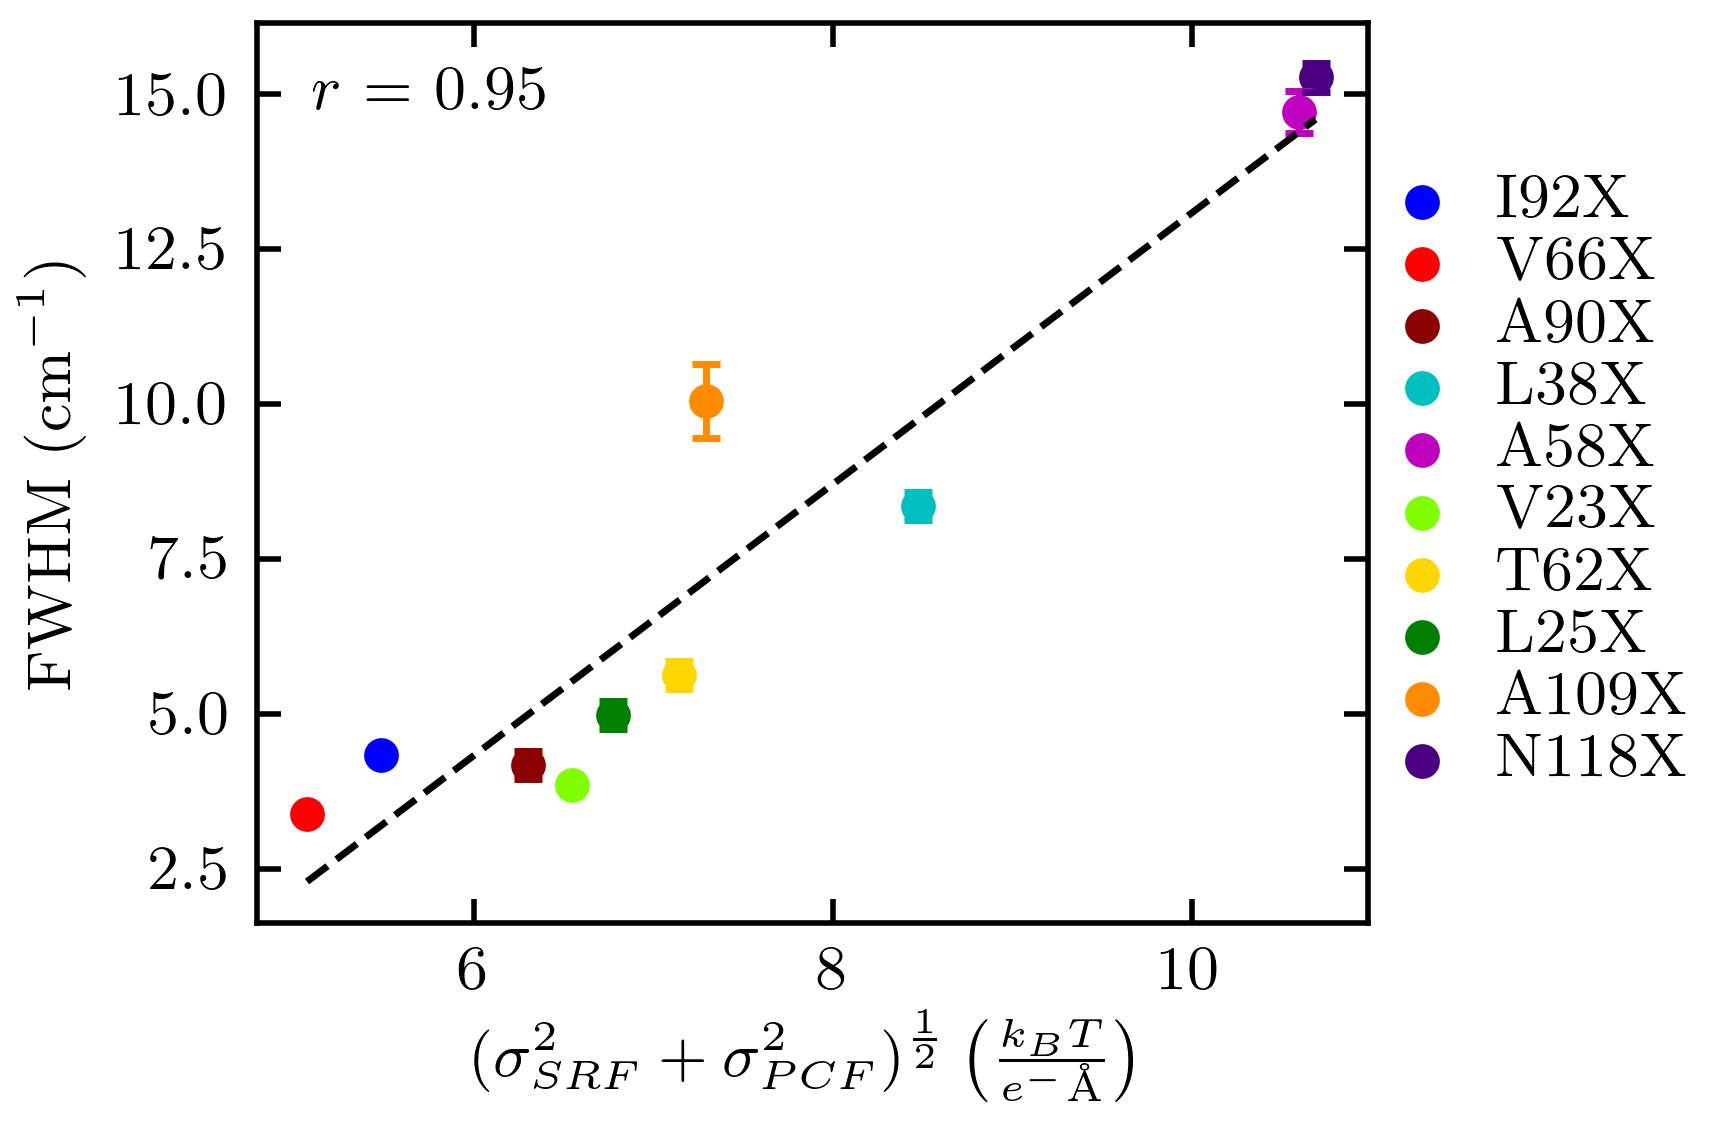
\includegraphics[width=\single]{figures-snase/fwhm_vs_std.png}
    \caption[Combined standard deviations of the component fields against the experimental FWHM]{
        The combined standard deviations of the calculated SRF and PCF against the experimental FWHM of the observed nitrile vibrational spectra. 
        The combined standard deviation was calculated from the standard deviations of each component of the field through Equation \ref{eq:snase-comb_std}.
    }
    \label{fig:snase-comb_std}
\end{figure}

To demonstrate this further, we binned the total external calculated field (PCF+SRF) and show the histogram of external fields in Figure \ref{fig:snase-broadened} (gray) in which the units of field have been converted from k$_\text{B}$T/e$^{-}$ \si{\angstrom} to \si{\wn} and centered underneath the observed mean frequency. 
The distributions of the total external field were qualitatively similar to the overall line shapes of the experimental spectra (black dashed lines, reproduced from Figure \ref{fig:snase-ftir}). 
For example, the histogram of the total external field for T62X contained a minor red-shifted population. 
Correspondingly, the vibrational spectrum of T62X contained a red-shifted shoulder, although to a lesser degree than indicated by the histogram of the external field. 
While the range of the widths of the histograms was smaller than the range of FWHMs of the experimental spectra, the histograms do not include broadening due to hydrogen bonding. 
Xu et al. demonstrated that the SolEFP model can accurately reproduce vibrational line shapes when convoluted with a classicized linear response function, which accounts for broadening due to the vibrational transition lifetime \cite{Xu2018}. 
Because nitrile vibrational lifetimes are affected by hydrogen bonding interactions \cite{vanWilderen2014}, we reasoned that the additional broadening observed in the experimental spectra was due in part to hydrogen bonding. 
Again, this is supported by the correlation between the FWHM of the spectral peaks and the experimentally measured FTLS (Figure \ref{fig:snase-ftls_vs_others}B). 

\begin{figure}
    \center
    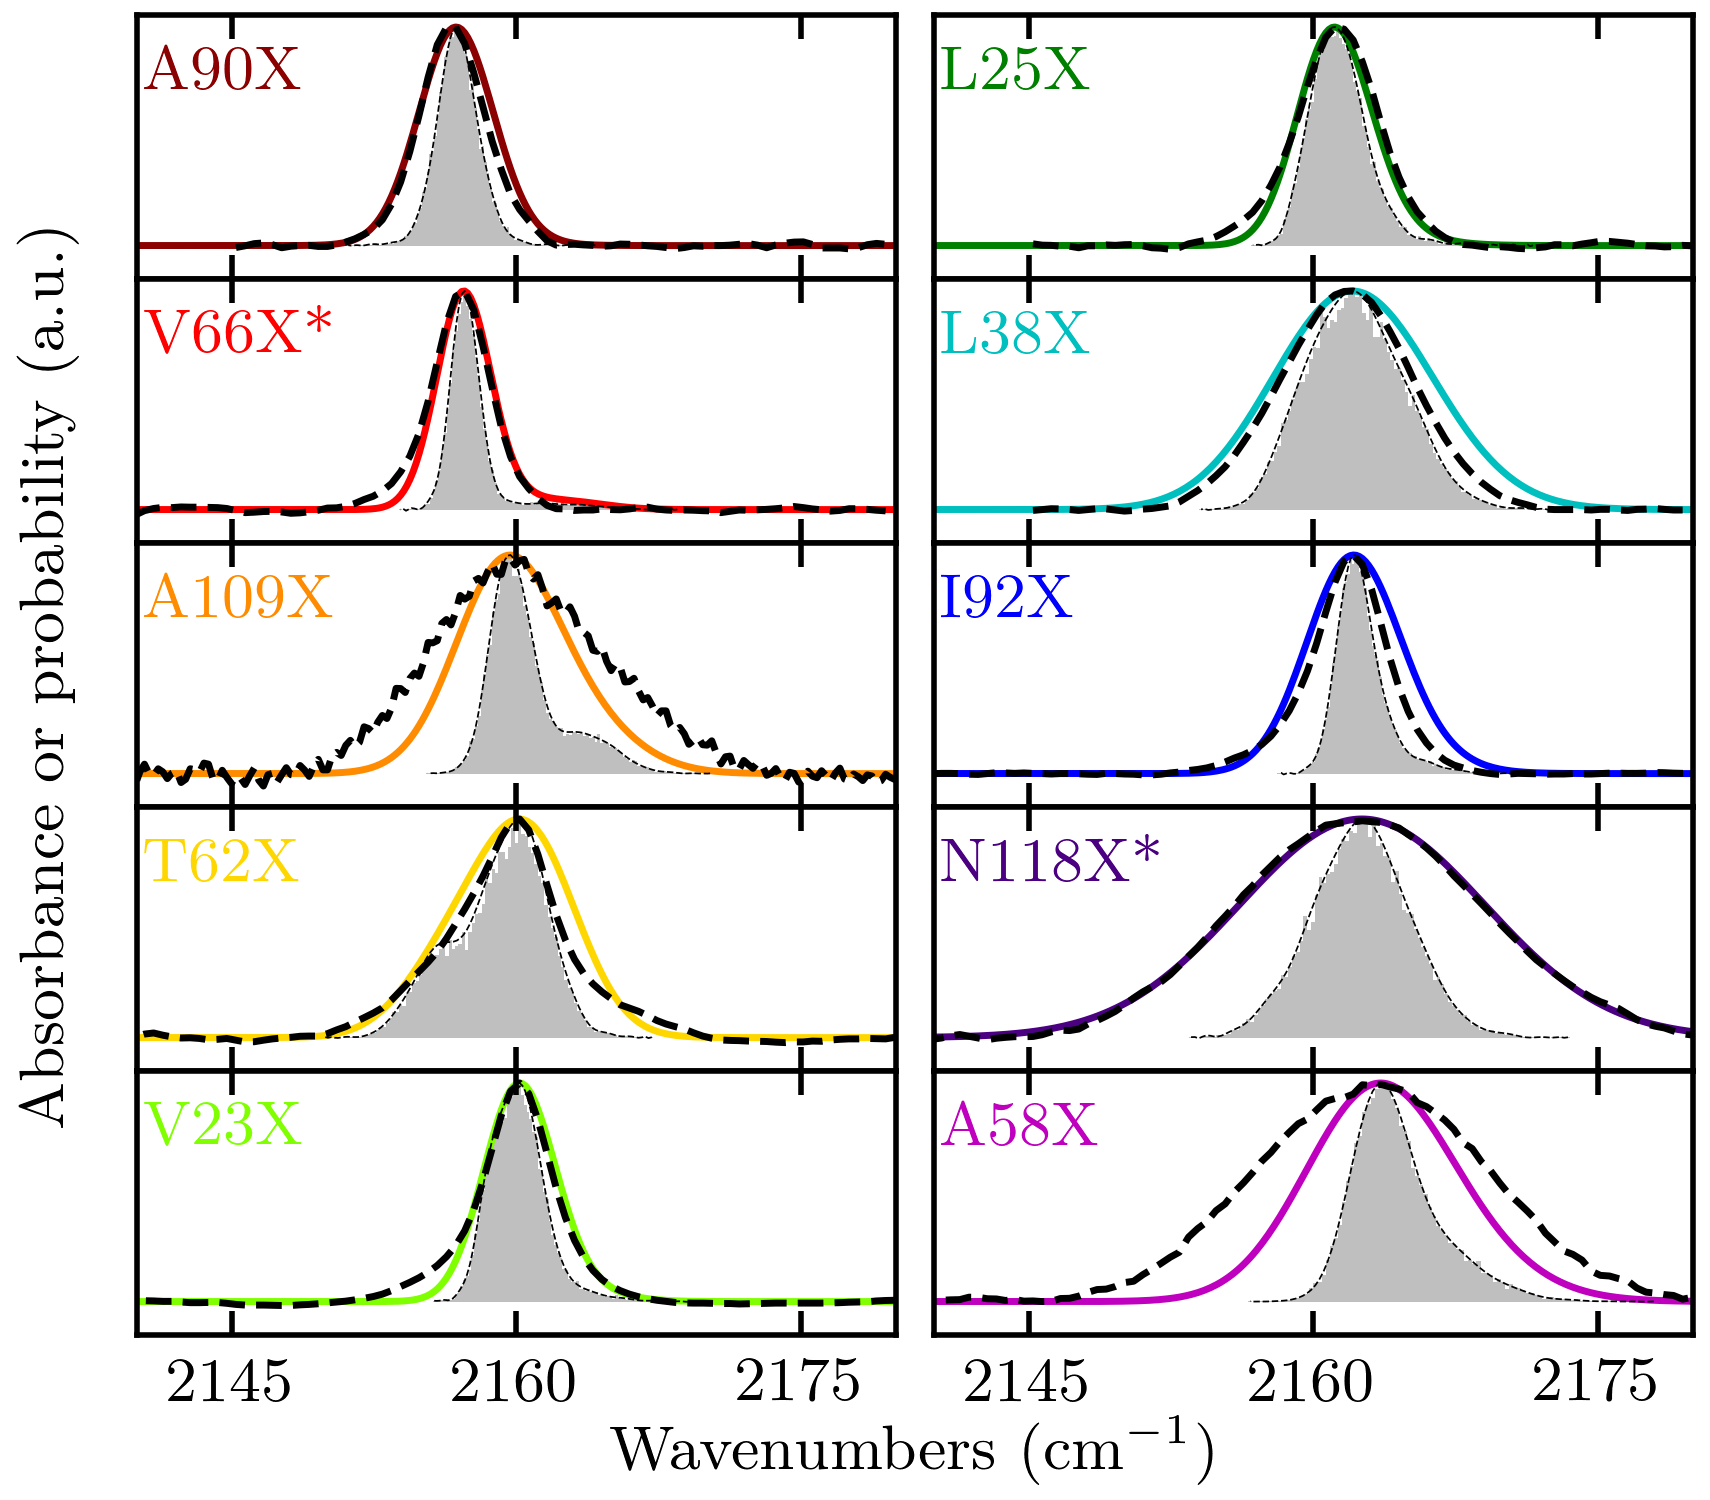
\includegraphics[width=\single]{figures-snase/convoluted_external_field.png}
    \caption[Broadened histograms of the total external field]{
        Broadened histograms of the total external field (SRF+PCF). 
        Gray: calculated histogram of the total field; 
        solid colored lines: sum of the broadened bins. 
        Each bin was broadened by a Gaussian with a bandwidth proportional to the experimental FTLS. 
        Dashed black lines: experimental spectra from Figure \ref{fig:snase-ftir} overlaid for reference.
    }
    \label{fig:snase-broadened}
\end{figure}

Because the FTLS of a nitrile provides quantitative information on the extent of hydrogen bonding, as demonstrated above, it can account for additional broadening not already captured by the field calculations. 
We therefore broadened each bin in the histograms of the total external field with a Gaussian in which the bandwidth was proportional to the experimentally measured FTLS, using the FWHM of V66X and N118X (the narrowest and widest spectra) to gauge the proportion. 
The broadened histograms are shown as solid colored lines in Figure \ref{fig:snase-broadened}. 
For most of the spectra, our broadened distributions qualitatively matched the experimentally observed line shapes. 
For example, using this analysis we can now more accurately represent the small shoulder in the T62X experimental spectrum, which was overestimated by the histogram of the external field. 
For A109X and A58X, however, the broadened field distribution seemed to underestimate the contribution of the more negative field (higher frequency). 
Nevertheless, the similarity between the broadened histograms and the experimentally measured vibrational spectra demonstrate that the details of the spectral line shape are important because they reveal the different microstates that the nitrile probe experiences. 
Even if classical fixed-charge force fields are unable to replicate overall shifts in vibrational frequencies, with the present MD simulations and orthogonal experimental measurements such as FTLS, we can qualitatively identify the populations of structures that give rise to these spectral features. 

We can begin to interpret these results quantitatively, as well, by tracking the FTLS of the individual populations that contribute to the overall spectra in the FTLS experiment. 
We tracked the temperature dependence of the individual Gaussians from a two-Gaussian fit for each temperature-dependent FTIR spectrum. 
The peak frequencies of these individual Gaussians were linearly dependent on the temperature, resulting in independent FTLS (Figure \ref{fig:snase-independent_ftls}). 
In principle, the FTLS of each particular population corresponds to a specific local environment sampled by the probe over the course of the steady-state experiment. 
For example, in the cases of N118X and A58X, the two Gaussians appeared to shift independently with increasing temperature, resulting in two different FTLS. 
We interpret this observation as corresponding to two populations, one in which the probe experiences more hydrogen bonding and therefore has a larger FTLS, and one with less hydrogen bonding and therefore has a smaller FTLS. 
Alternatively, there are several probe locations (A90X, V66X, V23X, L25X, and I92X) in which both Gaussians of the two-Gaussian fit result in a similar FTLS. 
In each of these spectra (Figure \ref{fig:snase-ftls_spectra}) there is only a single, narrow population. 
In these cases, this suggests that the probe predominately experiences a single population. 
This is supported by the MD, which showed single, narrow distributions of field with small amounts of hydrogen bonding. 
Interestingly, the spectra for T62X showed a clear shoulder population that increases in relative intensity with increasing temperature, but the peak frequencies of the two Gaussians have nearly the same FTLS. 
If one of these Gaussians corresponds to the population in which the probe experienced a strong hydrogen bond to water as described earlier, this supports our hypothesis that this particular hydrogen bond is insensitive to temperature changes in this range. 
Together, these observations suggest that FTLS could be used to monitor individual local environments sampled by the probe, beyond an ensemble average. 
We are currently exploring this idea further with temperature dependent MD.

\begin{figure}
    \center
    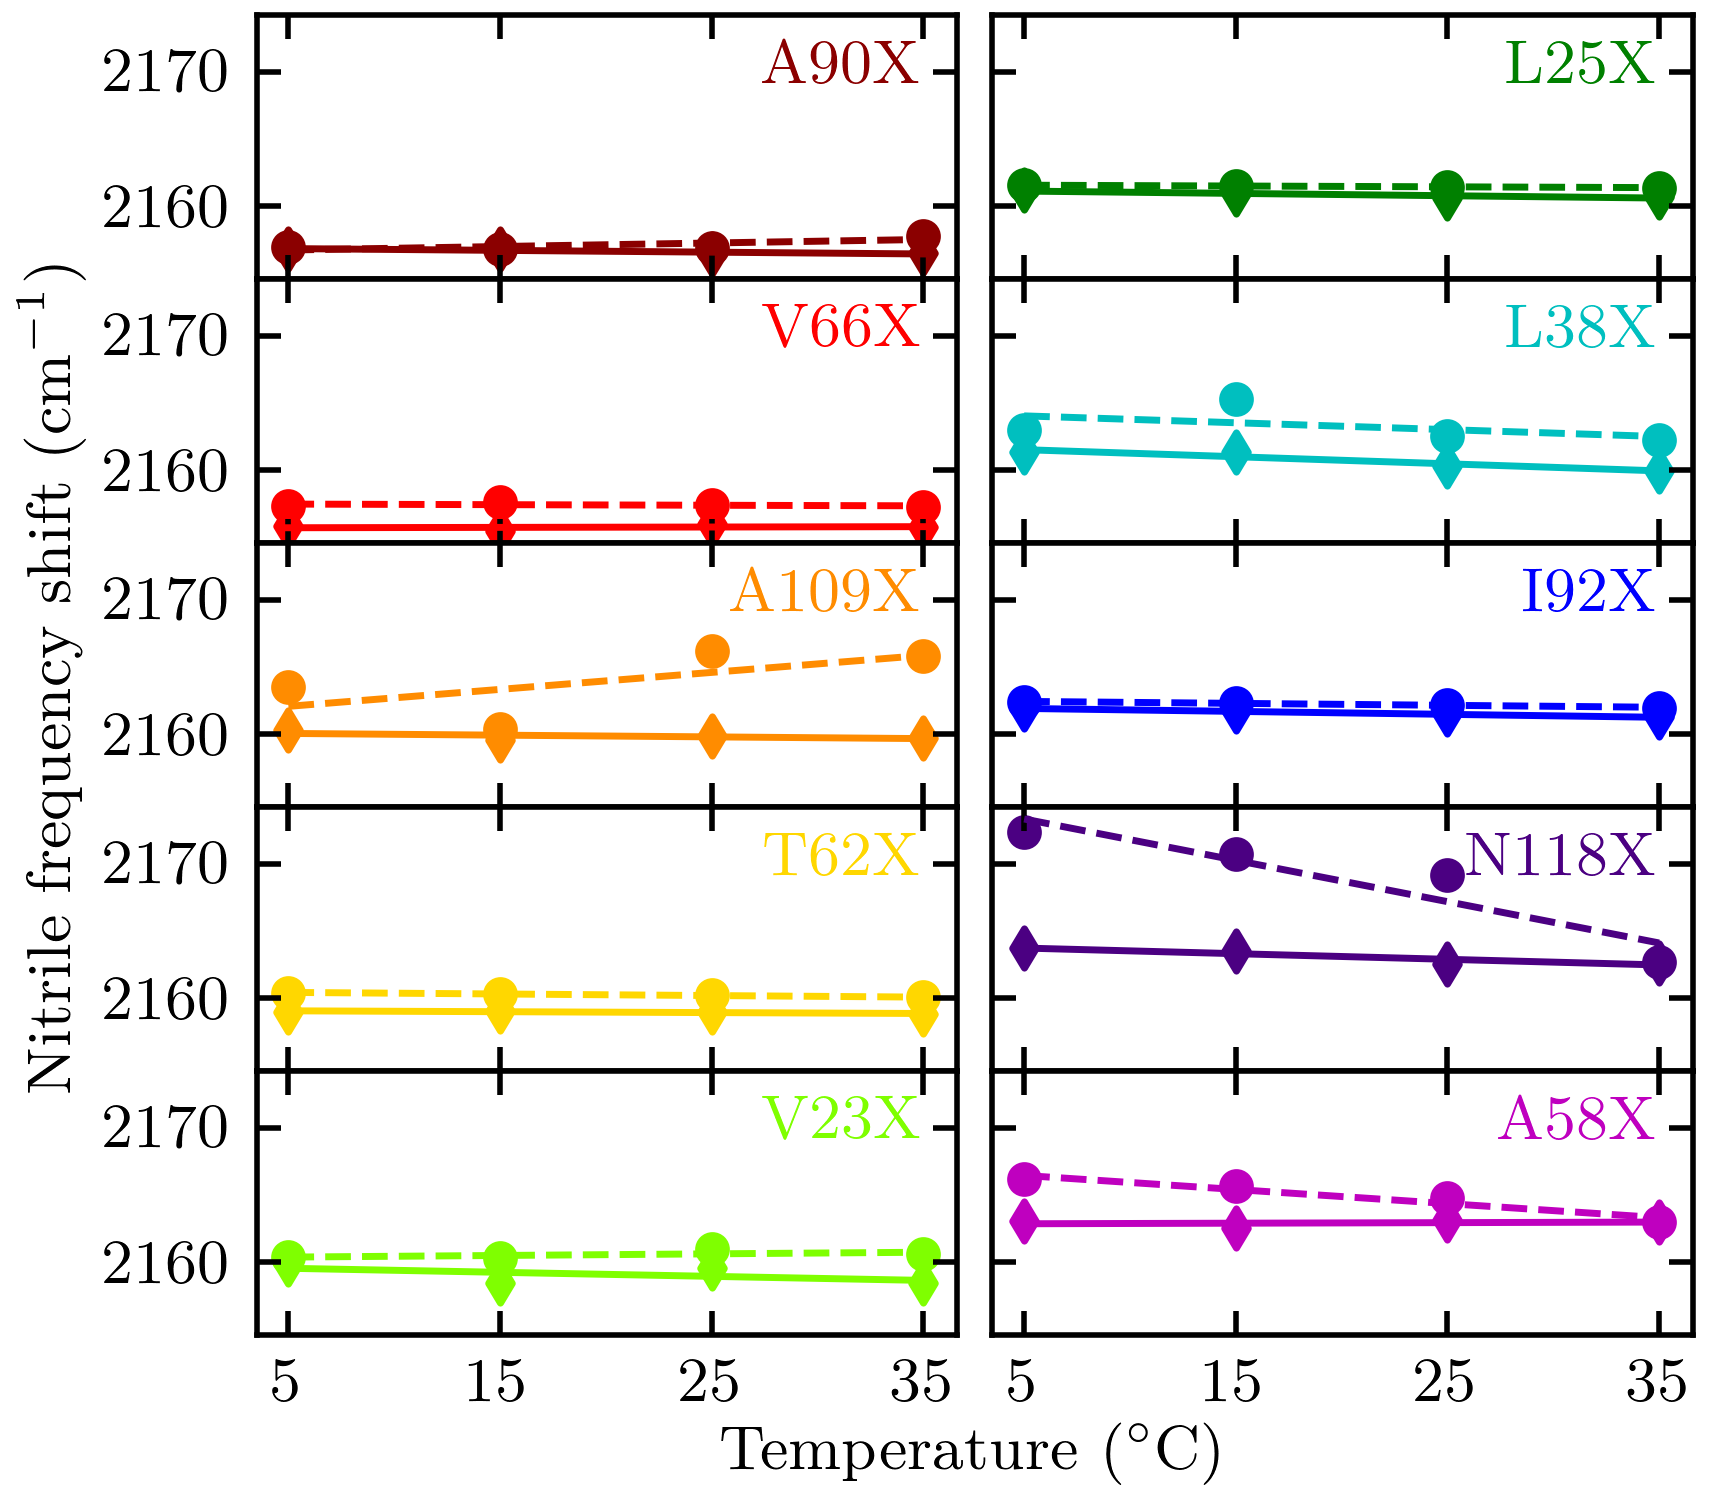
\includegraphics[width=\single]{figures-snase/ftls_both_gaussians.png}
    \caption[Independent FTLS from component populations of nitrile spectra]{
        Average of peak nitrile frequencies of two Gaussians fit to spectra collected from 5 \si{\celsius} to 35 \si{\celsius}. 
        Diamonds: frequency of the most blue-shifted Gaussian at each temperature. 
        Circles: frequency of the most red-shifted Gaussian at each temperature. 
        Solid lines are the linear fit to the blue-shifted peaks and dashed lines are the linear fit to the red-shifted peaks.
    }
    \label{fig:snase-independent_ftls}
\end{figure}

\begin{figure}
    \center
    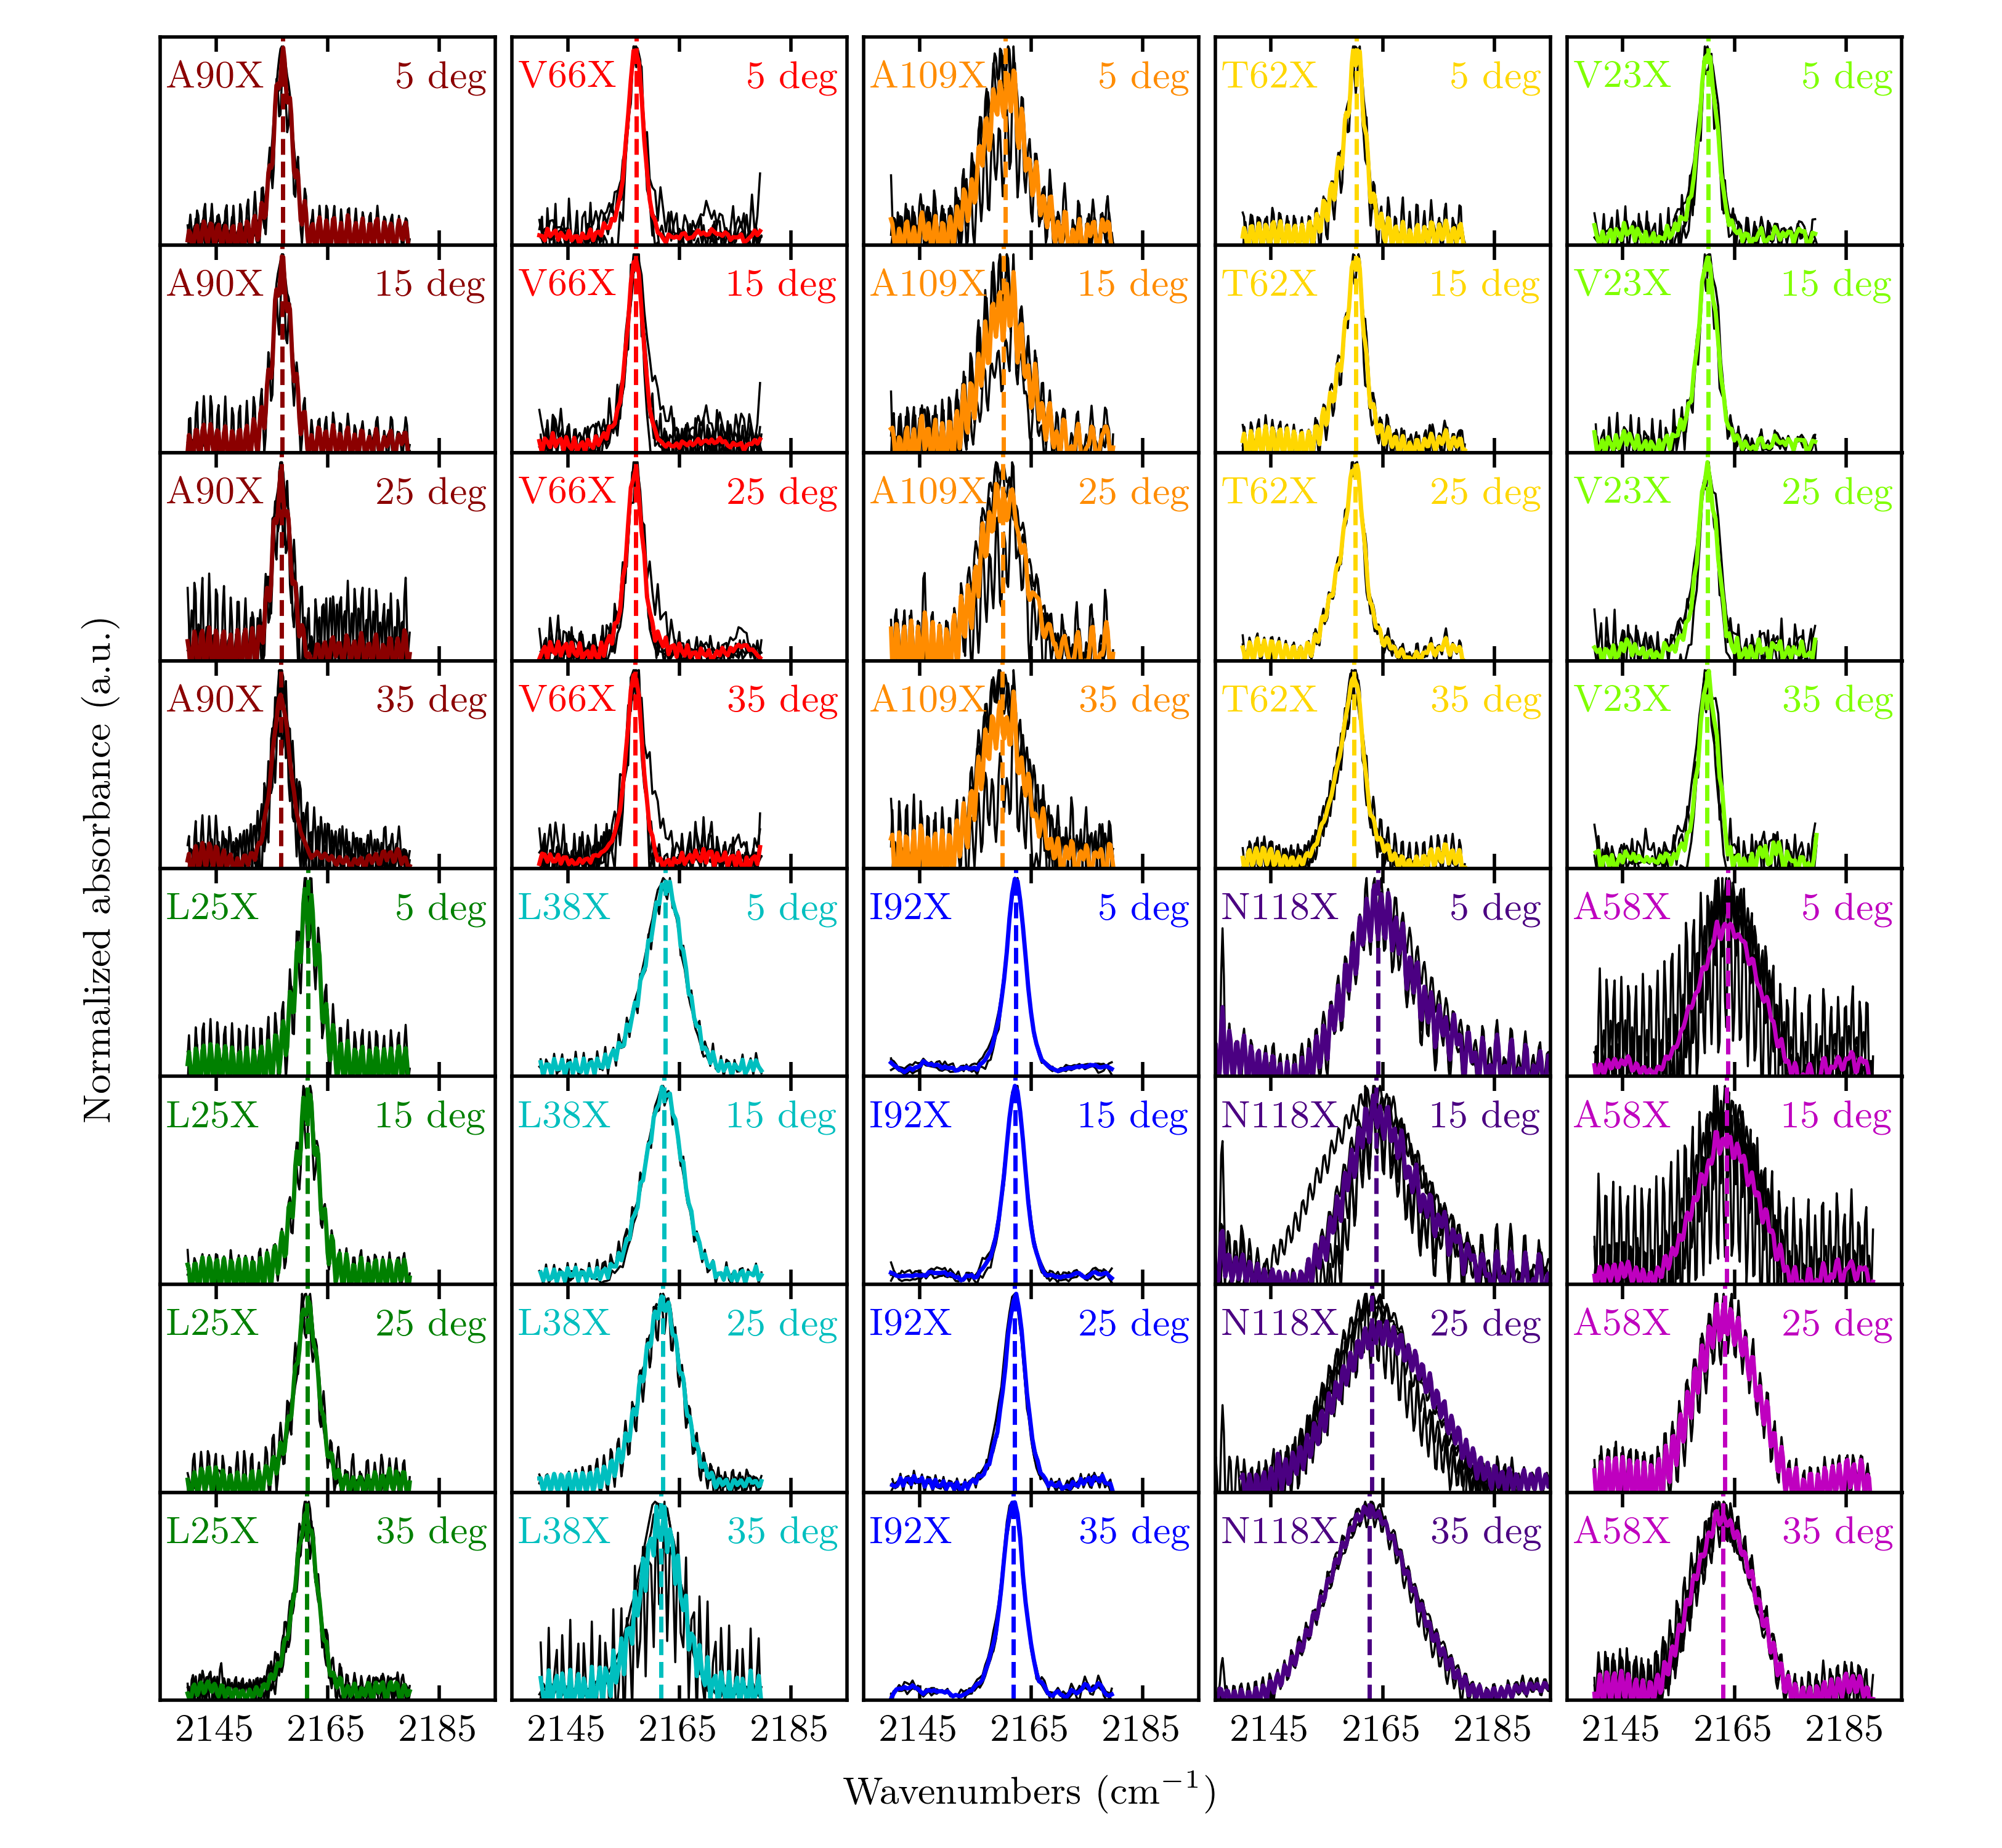
\includegraphics[width=\double]{figures-snase/ftls_all_spectra.png}
    \caption[]{
        FTIR absorption spectra of CNC incorporated at each of the ten locations from 5 \si{\celsius} to 35 \si{\celsius}. 
        The maximum absorbance of each spectrum was normalized to 1. 
        Colored lines: averaged absorption spectra; 
        black traces: individual FTIR spectra (some traces lie directly underneath the colored lines); 
        vertical dashed lines: peak frequency of the averaged spectra at the given temperature reported in Table \ref{tbl:snase-ftls}.
    }
    \label{fig:snase-ftls_spectra}
\end{figure}

The interpretation of nitrile spectra is complicated by the fact that the experimental nitrile stretching frequency is superimposed on top of a broader water absorption peak. 
Resolving the nitrile spectral line shape therefore requires a baseline correction that could systematically affect the observed line shape \cite{vanWilderen2014}. 
Though we observed agreement between broadened field calculations and experimental line shape, and the line shapes were reproducible, further quantitative investigation will require a more standardized approach to baseline correction and peak fitting. 
In spite of this, the vibrational line shape, FWHM, and FTLS were all self-consistent. 
In general, the suite of information offered by these experiments will be valuable for benchmarking methods for computing electrostatics moving forward.

In total, this work demonstrates that the overall vibrational frequencies of nitriles are difficult to relate to any one particular contribution. 
Specific hydrogen-bonding interactions, non-specific local interactions, and electric field all simultaneously contribute to the observed frequency. 
Indeed, Equation \ref{eq:snase-stark} reflects this, because only \emph{differences} in electric field may be related to \emph{differences} in vibrational frequency. 
However, in order to interpret differences in vibrational frequency in this manner, the overall environment of the nitrile must remain constant. 
For measurements in proteins, this is likely only possible when the nitrile location is consistent and perturbations are made around the nitrile probe \cite{Slocum2016, Stafford2012, Novelli2018}. 
Here, we have shown that in the case of a single nitrile-containing construct like any one of the SNase mutants in this study, it is difficult to interpret the relative vibrational frequency compared to the frequencies of nitrile probes in other locations. 
Nevertheless, the line shape of each nitrile spectrum can be used to identify individual populations for which the nitrile experiences a different projected field. 
By considering different populations for the same probe, it may be possible to interpret the distribution of frequencies inherent to a vibrational spectrum as differences in electric field according to Equation \ref{eq:snase-stark}. 
The similarities between the broadened histograms of the calculated external field and the spectral line shape in this study (Figure \ref{fig:snase-broadened}) demonstrate the feasibility of relating the electric field in different subpopulations to the line shape of a nitrile vibrational spectrum. 
Such close agreement between experiment and calculation demonstrates that only slightly more experimental information (i.e. FWHM and FTLS) with routine methodologies is required to interpret vibrational spectra quantitatively. 
This capability is greatly enhanced when experimental data can be compared to computational modeling as closely as possible.

%%%%%%%%%%%%%%%%%%%%%%%%%%%%%%%%%%%%%%%%%%%%%%%%%%%%%%%%%%%%%%%%
%%%%%%%%%%%%%%%%%%%%%%%%%%%%%%%%%%%%%%%%%%%%%%%%%%%%%%%%%%%%%%%%
\section{Conclusion} \label{snase-conclusion}
%%%%%%%%%%%%%%%%%%%%%%%%%%%%%%%%%%%%%%%%%%%%%%%%%%%%%%%%%%%%%%%%
%%%%%%%%%%%%%%%%%%%%%%%%%%%%%%%%%%%%%%%%%%%%%%%%%%%%%%%%%%%%%%%%

We have reported vibrational spectra of 10 nitrile-containing SNase mutants, where each nitrile was located at a position for which \dpKa{} information had previously been published. 
We found that the \pKa{}s for these locations were not in agreement with the observed nitrile vibrational frequencies. 
This is likely due to the different role of local interactions between the molecular probes, each of which is influenced by multiple factors from its own chemical structure. 
Differences in charge, dipole moment, hydrogen-bonding capabilities, flexibility, and size between each \pKa{} probe result in varied responses to both local and electrostatic factors. 
Using \pKa{} shifts to benchmark electrostatic models poses the risk of propagating these uncertainties. 
Instead, an uncharged, molecular probe, with a correspondingly smaller dipole moment, such as a nitrile, minimizes these convoluting factors. 
While the interpretation of nitrile frequencies is similarly complicated by hydrogen bonding interactions, we have demonstrated that the FTLS can be used to quantitatively diagnose the hydrogen bonding status of the nitrile within the protein. 
Furthermore, the line shape of the vibrational spectra contains important information about the differences in field between microstates of the probe that can be quantified from structural information from simulations.

In summary, nitrile vibrational spectra have the distinct advantage as a probe of electrostatic environment in that they: 
1) can be directly related to electric field through the Stark equation; 
2) offer additional information from the spectral line shape that indicates contributions from subpopulations of the probe; and 
3) can be quantitatively accounted for with additional experiments, such as measuring FTLS. 
This demonstrates that libraries of nitrile spectra are a valuable resource for benchmarking electrostatic computational models and, with the proper control experiments, for reporting quantitative information about electric fields in proteins. 
Further investigation of decoupling local interactions from overall electronic contributions to nitrile vibrational spectra will allow for a greater understanding and increased predictability of the complex electric fields that dominate biological systems.

